\documentclass[12pt]{book}
\usepackage[T1]{fontenc}
\usepackage{times}
\usepackage{listings}
\usepackage{graphicx}
\usepackage{xcolor}
\usepackage{url}
% \usepackage{showidx}
\usepackage{imakeidx}
\usepackage{booktabs}
\usepackage{url}
\usepackage{etoolbox}  % for showidx
\usepackage{fullpage}

\usepackage{hyperref}  % should be last

% One space after periods
\frenchspacing

\hypersetup{pdfauthor={Rus Cox, Frans Kaashoek, Robert Morris},
            pdftitle={xv6: a simple, Unix-like teaching operating system},}
  
\lstset{language=C,basicstyle=\small\ttfamily}
\lstset{morecomment=[is]{[[[}{]]]}}

\newcommand{\github}{https://github.com/kaashoek/xv6-risc-v/blob/riscv/}

\newcommand{\fileref}[1]{\href{\github/#1}{\small{(#1)}}}
\newcommand{\lineref}[2]{\href{\github/#1\#L#2}{\small{(#1:#2)}}}
\newcommand{\linerefs}[3]{\href{\github/#1\#L#2-L#3}{\small(#1:#2-#3)}}

\newcommand{\indextext}[1]{\textit{#1}\index{#1}}
\newcommand{\indexcode}[1]{\lstinline{#1}\index{#1@\lstinline{#1}}}

\title{\textbf{xv6: a simple, Unix-like teaching operating system}}
\author{Rus Cox \and Frans Kaashoek \and Robert Morris}

\makeindex

\begin{document}

\maketitle

\tableofcontents

\chapter*{Foreword and acknowledgements}


This is a draft text intended for a class on operating systems. It
explains the main concepts of operating systems by studying an example
kernel, named xv6.  xv6 is a re-implementation of Dennis Ritchie's and
Ken Thompson's Unix Version 6 (v6)~\cite{unix}.  xv6 loosely follows the structure
and style of v6, but is implemented in ANSI C~\cite{kernighan} for 
a multicore RISC-V.

This text should be read along with the source code for xv6, an approach 
inspired by John Lions's Commentary on UNIX 6th Edition~\cite{lions}. See
\url{https://pdos.csail.mit.edu/6.828} for pointers to on-line
resources for v6 and xv6, including several hands-on homework assignments
using xv6.

We have used this text in 6.828, the operating systems class at MIT.
We thank the faculty, teaching assistants, and students of 6.828 who
have all directly or indirectly contributed to xv6.  In particular, we
would like to thank Austin Clements and Nickolai Zeldovich.  Finally,
we would like to thank people who emailed us bugs in the text or
suggestions for improvements: Abutalib Aghayev, Sebastian Boehm, Anton
Burtsev, Raphael Carvalho, Rasit Eskicioglu, Color Fuzzy, Giuseppe,
Tao Guo, Robert Hilderman, Wolfgang Keller, Austin Liew, Pavan
Maddamsetti, Jacek Masiulaniec, Michael McConville, miguelgvieira,
Mark Morrissey, Harry Pan, Askar Safin, Salman Shah, Ruslan Savchenko,
Pawel Szczurko, Warren Toomey, tyfkda, tzerbib, and Zou Chang Wei.

If you spot errors or have suggestions for improvement, please send email to
Frans Kaashoek and Robert Morris (kaashoek,rtm@csail.mit.edu).

\chapter{Operating system interfaces}
\label{CH:UNIX}

The job of an operating system is to share a computer among
multiple programs and to provide a more useful set of services
than the hardware alone supports.
The operating system manages and abstracts
the low-level hardware, so that, for example,
a word processor need not concern itself with which type
of disk hardware is being used.
It also shares the hardware among multiple programs so
that they run (or appear to run) at the same time.
Finally, operating systems provide controlled ways for programs
to interact, so that they can share data or work together.

An operating system provides services to user programs through an interface.
\index{interface design}
Designing a good interface turns out to be
difficult.  On the one hand, we would like the interface to be
simple and narrow because that makes it easier to get the
implementation right.  On the other hand,
we may be tempted to offer many sophisticated features to applications.
The trick in
resolving this tension is to design interfaces that rely on a few
mechanisms that can be combined to provide much generality.

This book uses a single operating system as a concrete example to
illustrate operating system concepts.  That operating system,
xv6, provides the basic interfaces introduced by Ken Thompson and
Dennis Ritchie's Unix operating system~\cite{unix}, as well as mimicking Unix's
internal design.  Unix provides a
narrow interface whose mechanisms combine well, offering a surprising
degree of generality.  This interface has been so successful that
modern operating systems—BSD, Linux, Mac OS X, Solaris, and even, to a
lesser extent, Microsoft Windows—have Unix-like interfaces.
Understanding xv6 is a good start toward understanding any of these
systems and many others.

As shown in 
Figure~\ref{fig:os},
xv6 takes the traditional form of a
\indextext{kernel},
a special program that provides
services to running programs.
Each running program, called a
\indextext{process},
has memory containing instructions, data, and a stack. The
instructions implement the
program's computation.  The data are the variables on which
the computation acts. The stack organizes the program's procedure calls.

When a
process needs to invoke a kernel service, it invokes a procedure call
in the operating system interface.  Such a procedure is called a
\indextext{system call}.
The system call enters the kernel;
the kernel performs the service and returns.
Thus a process alternates between executing in
\indextext{user space}
and
\indextext{kernel space}.

The kernel uses the hardware protection mechanisms provided by a
CPU\footnote{
This text generally refers to the hardware element that executes a
computation with the term \indextext{CPU}, an acronym for central
processing unit.  Other documentation (e.g., the RISC-V specification)
also uses the words processor, core, and hart instead of CPU.
}
to
ensure that each process executing in user space can access only
its own memory.
The kernel executes with the hardware privileges required to
implement these protections; user programs execute without
those privileges.
When a user program invokes a system call, the hardware
raises the privilege level and starts executing a pre-arranged
function in the kernel.

\begin{figure}[t]
\center
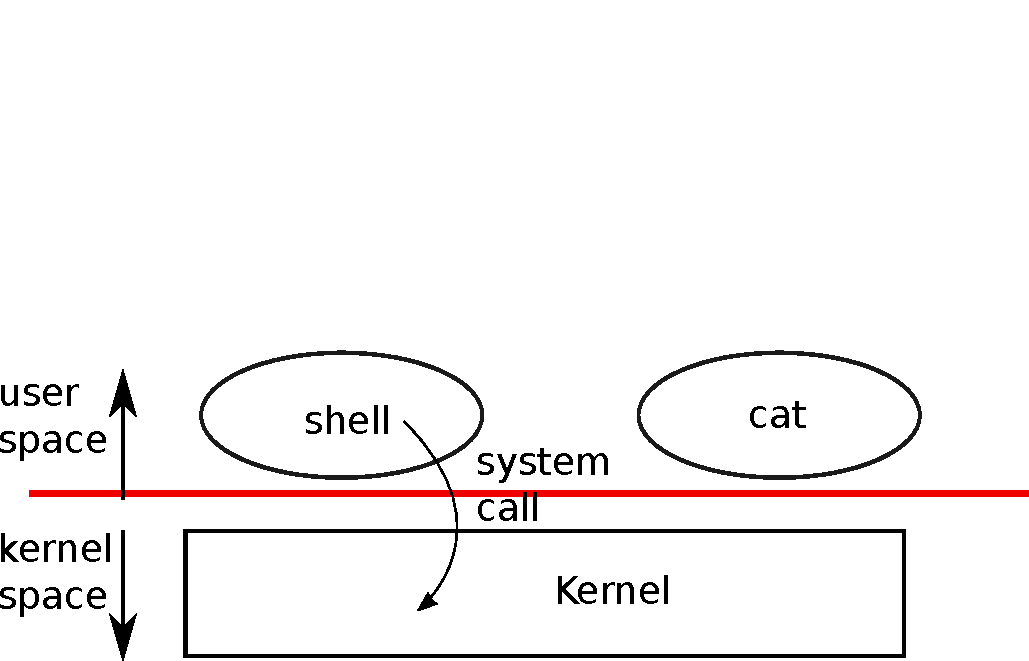
\includegraphics[scale=0.5]{fig/os.pdf}
\caption{A kernel and two user processes.}
\label{fig:os}
\end{figure}

The collection of system calls that a kernel provides
is the interface that user programs see.
The xv6 kernel provides a subset of the services and system calls
that Unix kernels traditionally offer.  
Figure~\ref{fig:api} 
lists all of xv6's system calls.

The rest of this chapter outlines xv6's services---processes, memory,
file descriptors, pipes, and a file system---and illustrates them with
code snippets and discussions of how the \indextext{shell}, which is
the primary user interface to traditional Unix-like systems, uses
them. The shell's use of system calls illustrates how carefully they
have been designed.

The shell is an ordinary program that reads commands from the user
and executes them.
The fact that the shell is a user program and not part of the kernel,
illustrates the power of the system call interface: there is nothing
special about the shell.
It also means that the shell is easy to replace; as a result,
modern Unix systems have a variety of
shells to choose from, each with its own user interface
and scripting features.
The xv6 shell is a simple implementation of the essence of
the Unix Bourne shell.  Its implementation can be found at 
\lineref{user/sh.c:1}.
%% 
%% 	Processes and memory
%% 
\section{Processes and memory}

An xv6 process consists of user-space memory (instructions, data, and stack)
and per-process state private to the kernel.
Xv6 can
\indextext{time-share} 
processes: it transparently switches the available CPUs
among the set of processes waiting to execute.
When a process is not executing, xv6 saves its CPU registers,
restoring them when it next runs the process.
The kernel associates a process identifier, or
\indexcode{pid},
with each process.

\begin{figure}[t]
\center
\begin{tabular}{ll}
{\bf System call} & {\bf Description} \\
\midrule
fork() & Create a process \\
exit(xstatus) & Terminate the current process with xstatus indicating success of failure \\
wait(*xstatus) & Wait for a child process to exit and copy the child's exit status to xstatus \\
kill(pid) & Terminate process pid \\
getpid() & Return the current process's pid \\
sleep(n) & Sleep for n clock ticks \\
exec(filename, *argv) & Load a file and execute it \\
sbrk(n) & Grow process's memory by n bytes \\
open(filename, flags) & Open a file; the flags indicate read/write \\
read(fd, buf, n) & Read n bytes from an open file into buf \\
write(fd, buf, n) & Write n bytes to an open file \\
close(fd) & Release open file fd \\
dup(fd) & Duplicate fd \\
pipe(p) & Create a pipe and return fd's in p \\
chdir(dirname) & Change the current directory \\
mkdir(dirname) & Create a new directory \\
mknod(name, major, minor) & Create a device file \\
fstat(fd) & Return info about an open file \\
link(f1, f2) & Create another name (f2) for the file f1 \\
unlink(filename) & Remove a file \\
\end{tabular}
\caption{Xv6 system calls}
\label{fig:api}
\end{figure}

A process may create a new process using the
\indexcode{fork}
system call.
\lstinline{Fork}
creates a new process, called the 
\indextext{child process}, 
with exactly the same memory contents
as the calling process, called the 
\indextext{parent process}.
\lstinline{Fork}
returns in both the parent and the child.
In the parent,
\indexcode{fork}
returns the child's pid;
in the child, it returns zero.
For example, consider the following program fragment written in the C
programming language~\cite{kernighan}:
\begin{lstlisting}[]
int pid = fork();
if(pid > 0){
  printf("parent: child=%d\n", pid);
  pid = wait(0);
  printf("child %d is done\n", pid);
} else if(pid == 0){
  printf("child: exiting\n");
  exit(0);
} else {
  printf("fork error\n");
}
\end{lstlisting}
The
\indexcode{exit}
system call causes the calling process to stop executing and
to release resources such as memory and open files.
Exit takes an integer status argument,
conventionally 0 to indicate success and 1 to indicate failure.
The
\indexcode{wait}
system call returns the pid of an exited child of the
current process and copies the exit status of the child to the address
passed to wait; if none of the caller's children
has exited,
\indexcode{wait}
waits for one to do so.
If the parent doesn't care about the exit status of a child, it can
pass a 0 address to
\lstinline{wait}.

In the example, the output lines
\begin{lstlisting}[]
parent: child=1234
child: exiting
\end{lstlisting}
might come out in either order, depending on whether the
parent or child gets to its
\indexcode{printf}
call first.
After the child exits the parent's
\indexcode{wait}
returns, causing the parent to print
\begin{lstlisting}[]
parent: child 1234 is done
\end{lstlisting}
Although the child has the same memory contents as the parent initially, the
parent and child are executing with different memory and different registers:
changing a variable in one does not affect the other. For example, when the
return value of
\lstinline{wait}
is stored into
\lstinline{pid} 
in the parent process,
it doesn't change the variable 
\lstinline{pid}
in the child.  The value of
\lstinline{pid}
in the child will still be zero.

The
\indexcode{exec}
system call
replaces the calling process's memory with a new memory
image loaded from a file stored in the file system.
The file must have a particular format, which specifies which part of
the file holds instructions, which part is data, at which instruction
to start, etc. xv6
uses the ELF format, which Chapter~\ref{CH:MEM} discusses in
more detail.
When
\indexcode{exec}
succeeds, it does not return to the calling program;
instead, the instructions loaded from the file start
executing at the entry point declared in the ELF header.
\lstinline{Exec}
takes two arguments: the name of the file containing the
executable and an array of string arguments.
For example:
\begin{lstlisting}[]
char *argv[3];

argv[0] = "echo";
argv[1] = "hello";
argv[2] = 0;
exec("/bin/echo", argv);
printf("exec error\n");
\end{lstlisting}
This fragment replaces the calling program with an instance
of the program 
\lstinline{/bin/echo}
running with the argument list
\lstinline{echo}
\lstinline{hello}.
Most programs ignore the first argument, which is 
conventionally the name of the program.

The xv6 shell uses the above calls to run programs on behalf of
users. The main structure of the shell is simple; see
\lstinline{main} 
\lineref{user/sh.c:/main/}.
The main loop reads a line of input from the user with
\indexcode{getcmd}.
Then it calls 
\lstinline{fork}, 
which creates a copy of the shell process. The
parent calls
\lstinline{wait},
while the child runs the command.  For example, if the user
had typed
``\lstinline{echo hello}''
to the shell,
\lstinline{runcmd}
would have been called with
``\lstinline{echo hello}''
as the argument.
\lstinline{runcmd} 
\lineref{user/sh.c:/runcmd/}
runs the actual command. For
``\lstinline{echo hello}'',
it would call
\lstinline{exec} 
\lineref{user/sh.c:/exec.ecmd/}.
If
\lstinline{exec}
succeeds then the child will execute instructions from
\lstinline{echo}
instead of
\lstinline{runcmd}.  
At some point
\lstinline{echo}
will call
\lstinline{exit},
which will cause the parent to return from
\lstinline{wait}
in 
\lstinline{main}
\lineref{user/sh.c:/main/}.

You might wonder why
\indexcode{fork}
and
\indexcode{exec}
are not combined in a single call; we will see later that separate
calls for creating a process and loading a program has some clever
usages in the shell for I/O redirection.  To avoid the wastefulness of
creating a duplicate process and then immediately replacing it,
operating kernels optimize the implementation of
\lstinline{fork}
for this use case by using virtual memory techniques such as
copy-on-write\mfk{need forward-reference and need to actually describe
  what COW is}.

Xv6 allocates most user-space memory
implicitly:
\indexcode{fork}
allocates the memory required for the child's copy of the
parent's memory, and 
\indexcode{exec}
allocates enough memory to hold the executable file.
A process that needs more memory at run-time (perhaps for
\indexcode{malloc})
can call
\lstinline{sbrk(n)}
to grow its data memory by
\lstinline{n}
bytes;
\indexcode{sbrk}
returns the location of the new memory.

Xv6 does not provide a notion of users or of protecting
one user from another; in Unix terms, all xv6 processes
run as root.
%% 
%% 	I/O and File descriptors
%% 
\section{I/O and File descriptors}

A 
\indextext{file descriptor} 
is a small integer representing a kernel-managed object
that a process may read from or write to.
A process may obtain a file descriptor by opening a file, directory,
or device, or by creating a pipe, or by duplicating an existing
descriptor.
For simplicity we'll often refer to the object a file descriptor
refers to as a ``file'';
the file descriptor interface abstracts away the differences between
files, pipes, and devices, making them all look like streams of bytes.
We'll refer to input and output as \indextext{I/O}.

Internally, the xv6 kernel uses the file descriptor
as an index into a per-process table,
so that every process has a private space of file descriptors
starting at zero.
By convention, a process reads from file descriptor 0 (standard input),
writes output to file descriptor 1 (standard output), and
writes error messages to file descriptor 2 (standard error).
As we will see, the shell exploits the convention to implement I/O redirection
and pipelines. The shell ensures that it always has three file descriptors
open
\lineref{user/sh.c:/open..console/},
which are by default file descriptors for the console.

The
\lstinline{read}
and
\lstinline{write}
system calls read bytes from and write bytes to
open files named by file descriptors.
The call
\lstinline{read(fd},
\lstinline{buf},
\lstinline{n)}
reads at most
\lstinline{n}
bytes from the file descriptor
\lstinline{fd},
copies them into
\lstinline{buf},
and returns the number of bytes read.
Each file descriptor that refers to a file
has an offset associated with it.
\lstinline{Read}
reads data from the current file offset and then advances
that offset by the number of bytes read:
a subsequent
\lstinline{read}
will return the bytes following the ones returned by the first
\lstinline{read}.
When there are no more bytes to read,
\lstinline{read}
returns zero to indicate the end of the file.

The call
\lstinline{write(fd},
\lstinline{buf},
\lstinline{n)}
writes
\lstinline{n}
bytes from
\lstinline{buf}
to the file descriptor
\lstinline{fd}
and returns the number of bytes written.
Fewer than
\lstinline{n}
bytes are written only when an error occurs.
Like
\lstinline{read},
\lstinline{write}
writes data at the current file offset and then advances
that offset by the number of bytes written:
each
\lstinline{write}
picks up where the previous one left off.

The following program fragment (which forms the essence of the program
\lstinline{cat})
copies data from its standard input
to its standard output.  If an error occurs, it writes a message
to the standard error.
\begin{lstlisting}[]
char buf[512];
int n;

for(;;){
  n = read(0, buf, sizeof buf);
  if(n == 0)
    break;
  if(n < 0){
    fprintf(2, "read error\n");
    exit();
  }
  if(write(1, buf, n) != n){
    fprintf(2, "write error\n");
    exit();
  }
}
\end{lstlisting}
The important thing to note in the code fragment is that
\lstinline{cat}
doesn't know whether it is reading from a file, console, or a pipe.
Similarly 
\lstinline{cat}
doesn't know whether it is printing to a console, a file, or whatever.
The use of file descriptors and the convention that file descriptor 0
is input and file descriptor 1 is output allows a simple
implementation
of 
\lstinline{cat}.

The
\lstinline{close}
system call
releases a file descriptor, making it free for reuse by a future
\lstinline{open},
\lstinline{pipe},
or
\lstinline{dup}
system call (see below).
A newly allocated file descriptor 
is always the lowest-numbered unused
descriptor of the current process.

File descriptors and
\indexcode{fork}
interact to make I/O redirection easy to implement.
\lstinline{Fork}
copies the parent's file descriptor table along with its memory,
so that the child starts with exactly the same open files as the parent.
The system call
\indexcode{exec}
replaces the calling process's memory but preserves its file table.
This behavior allows the shell to
implement \indextext{I/O redirection} by forking, reopening chosen file descriptors,
and then execing the new program.
Here is a simplified version of the code a shell runs for the
command
\lstinline{cat}
\lstinline{<}
\lstinline{input.txt}:
\begin{lstlisting}[]
char *argv[2];

argv[0] = "cat";
argv[1] = 0;
if(fork() == 0) {
  close(0);
  open("input.txt", O_RDONLY);
  exec("cat", argv);
}
\end{lstlisting}
After the child closes file descriptor 0,
\lstinline{open}
is guaranteed to use that file descriptor
for the newly opened
\lstinline{input.txt}:
0 will be the smallest available file descriptor.
\lstinline{Cat}
then executes with file descriptor 0 (standard input) referring to
\lstinline{input.txt}.

The code for I/O redirection in the xv6 shell works in exactly this way
\lineref{user/sh.c:/case.REDIR/}.
Recall that at this point in the code the shell has already forked the
child shell and that 
\lstinline{runcmd} 
will call
\lstinline{exec}
to load the new program.  Now it should be clear why it is a good idea that
\lstinline{fork}
and 
\lstinline{exec} 
are separate calls.  Because if they are separate, the shell can fork a child,
use
\lstinline{open},
\lstinline{close},
\lstinline{dup}
in the child to change the standard input and output
file descriptors, and then
\lstinline{exec}.
No changes to the program being exec-ed
(\lstinline{cat}
in our example)
are required.
If
\lstinline{fork}
and
\lstinline{exec}
were combined into a single
system call, some other (probably more complex) scheme would be required for the
shell to redirect standard input and output, or the program itself would have to
understand how to redirect I/O.

Although
\lstinline{fork}
copies the file descriptor table, each underlying file offset is shared
between parent and child.
Consider this example:
\begin{lstlisting}[]
if(fork() == 0) {
  write(1, "hello ", 6);
  exit(0);
} else {
  wait(0);
  write(1, "world\n", 6);
}
\end{lstlisting}
At the end of this fragment, the file attached to file descriptor 1
will contain the data
\lstinline{hello}
\lstinline{world}.
The
\lstinline{write}
in the parent
(which, thanks to
\lstinline{wait},
runs only after the child is done)
picks up where the child's
\lstinline{write}
left off.
This behavior helps produce sequential output from sequences
of shell commands, like
\lstinline{(echo}
\lstinline{hello};
\lstinline{echo}
\lstinline{world)}
\lstinline{>output.txt}.

The
\lstinline{dup}
system call duplicates an existing file descriptor,
returning a new one that refers to the same underlying I/O object.
Both file descriptors share an offset, just as the file descriptors
duplicated by
\lstinline{fork}
do.
This is another way to write
\lstinline{hello}
\lstinline{world}
into a file:
\begin{lstlisting}[]
fd = dup(1);
write(1, "hello ", 6);
write(fd, "world\n", 6);
\end{lstlisting}

Two file descriptors share an offset if they were derived from
the same original file descriptor by a sequence of
\lstinline{fork}
and
\lstinline{dup}
calls.
Otherwise file descriptors do not share offsets, even if they
resulted from 
\lstinline{open}
calls for the same file.  
\lstinline{Dup} 
allows shells to implement commands like this:
\lstinline{ls}
\lstinline{existing-file}
\lstinline{non-existing-file}
\lstinline{>}
\lstinline{tmp1}
\lstinline{2>&1}.
The
\lstinline{2>&1}
tells the shell to give the command a file descriptor 2 that
is a duplicate of descriptor 1.
Both the name of the existing file and the error message for the
non-existing file will show up in the file
\lstinline{tmp1}.
The xv6 shell doesn't support I/O redirection for the error file
descriptor, but now you know how to implement it.

File descriptors are a powerful abstraction,
because they hide the details of what they are connected to:
a process writing to file descriptor 1 may be writing to a
file, to a device like the console, or to a pipe.
%% 
%% 	Pipes
%% 
\section{Pipes}

A 
\indextext{pipe} 
is a small kernel buffer exposed to processes as a pair of
file descriptors, one for reading and one for writing.
Writing data to one end of the pipe
makes that data available for reading from the other end of the pipe.
Pipes provide a way for processes to communicate.

The following example code runs the program
\lstinline{wc}
with standard input connected to
the read end of a pipe.
\begin{lstlisting}[]
int p[2];
char *argv[2];

argv[0] = "wc";
argv[1] = 0;

pipe(p);
if(fork() == 0) {
  close(0);
  dup(p[0]);
  close(p[0]);
  close(p[1]);
  exec("/bin/wc", argv);
} else {
  close(p[0]);
  write(p[1], "hello world\n", 12);
  close(p[1]);
}
\end{lstlisting}
The program calls
\lstinline{pipe},
which creates a new pipe and records the read and write
file descriptors in the array
\lstinline{p}.
After
\lstinline{fork},
both parent and child have file descriptors referring to the pipe.
The child dups the read end onto file descriptor 0,
closes the file descriptors in
\lstinline{p},
and execs
\lstinline{wc}.
When 
\lstinline{wc}
reads from its standard input, it reads from the pipe.
The parent closes the read side of the pipe,
writes to the pipe,
and then closes the write side.

If no data is available, a
\lstinline{read}
on a pipe waits for either data to be written or all
file descriptors referring to the write end to be closed;
in the latter case,
\lstinline{read}
will return 0, just as if the end of a data file had been reached.
The fact that
\lstinline{read}
blocks until it is impossible for new data to arrive
is one reason that it's important for the child to
close the write end of the pipe
before executing
\lstinline{wc}
above: if one of
\lstinline{wc} 's
file descriptors referred to the write end of the pipe,
\lstinline{wc}
would never see end-of-file.

The xv6 shell implements pipelines such as
\lstinline{grep fork sh.c | wc -l}
in a manner similar to the above code
\lineref{user/sh.c:/case.PIPE/}.
The child process creates a pipe to connect the left end of the pipeline
with the right end. Then it calls
\lstinline{fork}
and
\lstinline{runcmd}
for the left end of the pipeline
and 
\lstinline{fork}
and
\lstinline{runcmd}
for the right end, and waits for both to finish.
The right end of the pipeline may be a command that itself includes a
pipe (e.g.,
\lstinline{a}
\lstinline{|}
\lstinline{b}
\lstinline{|}
\lstinline{c)}, 
which itself forks two new child processes (one for
\lstinline{b}
and one for
\lstinline{c}).
Thus, the shell may
create a tree of processes.  The leaves of this tree are commands and
the interior nodes are processes that wait until the left and right
children complete.

In principle, one could have the interior nodes run the left end of a
pipeline, but doing so correctly would complicate the
implementation. Consider making just the following modification:
change \lstinline{sh.c} to not fork for \lstinline{p->left} and run
\lstinline{runcmd(p->left)} in the interior process. Then, for
example, \lstinline{echo hi | wc} won't produce output, because when
\lstinline{echo hi} exits in \lstinline{runcmd}, the interior process
exits and never calls fork to run the right end of the pipe.  This
incorrect behavior could be fixed by not calling \lstinline{exit} in
\lstinline{runcmd} for interior processes, but this fix complicates
the code: now \lstinline{runcmd} needs to know if it a interior
process or not.  Complications also arise when not forking for
\lstinline{runcmd(p->right)}.  For example, with just that modification,
\lstinline{sleep 10 | echo hi} will immediately print ``hi'' instead
of after 10 seconds, because \lstinline{echo} runs immediately and
exits, not waiting for \lstinline{sleep} to finish.  Since the goal of
the \lstinline{sh.c} is to be as simple as possible, it doesn't try to
avoid creating interior processes.

Pipes may seem no more powerful than temporary files:
the pipeline
\begin{lstlisting}[]
echo hello world | wc
\end{lstlisting}
could be implemented without pipes as
\begin{lstlisting}[]
echo hello world >/tmp/xyz; wc </tmp/xyz
\end{lstlisting}
Pipes have at least four advantages over temporary files
in this situation.
First, pipes automatically clean themselves up;
with the file redirection, a shell would have to
be careful to remove
\lstinline{/tmp/xyz}
when done.
Second, pipes can pass arbitrarily long streams of
data, while file redirection requires enough free space
on disk to store all the data.
Third, pipes allow for parallel execution of pipeline stages,
while the file approach requires the first program to finish
before the second starts.
Fourth, if you are implementing inter-process communication,
pipes' blocking reads and writes are more efficient
than the non-blocking semantics of files.
%% 
%% 	File system
%% 
\section{File system}

The xv6 file system provides data files,
which are uninterpreted byte arrays,
and directories, which
contain named references to data files and other directories.
The directories form a tree, starting
at a special directory called the 
\indextext{root}.
A 
\indextext{path} 
like
\lstinline{/a/b/c}
refers to the file or directory named
\lstinline{c}
inside the directory named
\lstinline{b}
inside the directory named
\lstinline{a}
in the root directory
\lstinline{/}.
Paths that don't begin with
\lstinline{/}
are evaluated relative to the calling process's
\indextext{current directory},
which can be changed with the
\lstinline{chdir}
system call.
Both these code fragments open the same file
(assuming all the directories involved exist):
\begin{lstlisting}[]
chdir("/a");
chdir("b");
open("c", O_RDONLY);

open("/a/b/c", O_RDONLY);
\end{lstlisting}
The first fragment changes the process's current directory to
\lstinline{/a/b};
the second neither refers to nor changes the process's current directory.

There are multiple system calls to create a new file or directory:
\lstinline{mkdir}
creates a new directory,
\lstinline{open}
with the
\lstinline{O_CREATE}
flag creates a new data file,
and
\lstinline{mknod}
creates a new device file.
This example illustrates all three:
\begin{lstlisting}[]
mkdir("/dir");
fd = open("/dir/file", O_CREATE|O_WRONLY);
close(fd);
mknod("/console", 1, 1);
\end{lstlisting}
\lstinline{Mknod}
creates a file in the file system,
but the file has no contents.
Instead, the file's metadata marks it as a device file
and records the major and minor device numbers
(the two arguments to 
\lstinline{mknod}),
which uniquely identify a kernel device.
When a process later opens the file, the kernel
diverts
\lstinline{read}
and
\lstinline{write}
system calls to the kernel device implementation
instead of passing them to the file system.

\lstinline{Fstat}
retrieves information about the object a file
descriptor refers to.
It fills in a
\lstinline{struct}
\lstinline{stat},
defined in
\lstinline{stat.h} \fileref{kernel/stat.h}
as:
\begin{lstlisting}[]
#define T_DIR     1   // Directory
#define T_FILE    2   // File
#define T_DEVICE  3   // Device

struct stat {
  int dev;     // File system's disk device
  uint ino;    // Inode number
  short type;  // Type of file
  short nlink; // Number of links to file
  uint64 size; // Size of file in bytes
};
\end{lstlisting}

A file's name is distinct from the file itself;
the same underlying file, called an 
\indextext{inode}, 
can have multiple names,
called 
\indextext{links}.
The
\lstinline{link}
system call creates another file system name 
referring to the same inode as an existing file.
This fragment creates a new file named both
\lstinline{a}
and
\lstinline{b}.
\begin{lstlisting}[]
open("a", O_CREATE|O_WRONLY);
link("a", "b");
\end{lstlisting}
Reading from or writing to
\lstinline{a}
is the same as reading from or writing to
\lstinline{b}.
Each inode is identified by a unique
\textit{inode}
\textit{number}.
After the code sequence above, it is possible
to determine that
\lstinline{a}
and
\lstinline{b}
refer to the same underlying contents by inspecting the
result of 
\lstinline{fstat}:
both will return the same inode number 
(\lstinline{ino}),
and the
\lstinline{nlink}
count will be set to 2.

The
\lstinline{unlink}
system call removes a name from the file system.
The file's inode and the disk space holding its content
are only freed when the file's link count is zero and
no file descriptors refer to it.
Thus adding
\begin{lstlisting}[]
unlink("a");
\end{lstlisting}
to the last code sequence leaves the inode
and file content accessible as
\lstinline{b}.
Furthermore,
\begin{lstlisting}[]
fd = open("/tmp/xyz", O_CREATE|O_RDWR);
unlink("/tmp/xyz");
\end{lstlisting}
is an idiomatic way to create a temporary inode 
that will be cleaned up when the process closes 
\lstinline{fd}
or exits.

Shell commands for file system operations are implemented
as user-level programs such as
\lstinline{mkdir},
\lstinline{ln},
\lstinline{rm},
etc. This design allows anyone to extend the shell with new user commands by
just adding a new user-level program.  In hindsight this plan seems obvious,
but other systems designed at the time of Unix often built such commands into
the shell (and built the shell into the kernel).

One exception is
\lstinline{cd},
which is built into the shell
\lineref{user/sh.c:/if.buf.0..==..c./}.
\lstinline{cd}
must change the current working directory of the
shell itself.  If
\lstinline{cd}
were run as a regular command, then the shell would fork a child
process, the child process would run
\lstinline{cd},
and
\lstinline{cd}
would change the 
\textit{child} 's 
working directory.  The parent's (i.e.,
the shell's) working directory would not change.
%% 
%% 	Real world
%% 
\section{Real world}

Unix's combination of ``standard'' file
descriptors, pipes, and convenient shell syntax for
operations on them was a major advance in writing
general-purpose reusable programs.
The idea sparked a whole culture of ``software tools'' that was
responsible for much of Unix's power and popularity,
and the shell was the first so-called ``scripting language.''
The Unix system call interface persists today in systems like
BSD, Linux, and Mac OS X.

The Unix system call interface has been standardized through the Portable
Operating System Interface (POSIX) standard.
Xv6 is
\textit{not}
POSIX compliant.  It misses system calls (including basic ones such as
\lstinline{lseek}),
it implements system calls only partially, as well as other differences.  Our main goals for xv6 are
simplicity and clarity while providing a simple UNIX-like system-call interface.
Several people have extended xv6 with a few more system calls and a simple
C library in order to run basic Unix programs.  Modern kernels, however,
provide many more system calls, and many more kinds of kernel services, than
xv6.  For example, they support networking, windowing systems, user-level threads,
drivers for many devices, and so on.  Modern kernels evolve continuously and
rapidly, and offer many features beyond POSIX.

For the most part, modern Unix-derived operating systems
have not followed the early
Unix model of exposing devices as special files, like the
\lstinline{console}
device file discussed above.
The authors of Unix went on to build Plan 9,
which applied the ``resources are files''
concept to modern facilities,
representing networks, graphics, and other resources
as files or file trees.

The file system and file descriptors have been  powerful
abstractions.
Even so, there are other models for operating system interfaces.
Multics, a predecessor of Unix,
abstracted file storage in a way that made it look like memory,
producing a very different flavor of interface.
The complexity of the Multics design had a direct influence
on the designers of Unix, who tried to build something simpler.
% XXX can we cut this, since its point is the same as the next paragraph?
% An operating system interface that went out of fashion
% decades ago but has recently returned is the idea of a virtual machine monitor.
% Such systems provide a superficially different interface from xv6,
% but the basic concepts are still the same:
% a virtual machine, like a process, consists of some memory and
% one or more register sets;
% the virtual machine has access to one large file called
% a virtual disk instead of a file system;
% virtual machines send messages to each other
% and the outside world using virtual network devices
% instead of pipes or files.

This book examines how xv6 implements its Unix-like interface,
but the ideas and concepts apply to more than just Unix.
Any operating system must multiplex processes onto
the underlying hardware, isolate processes from each
other, and provide mechanisms for controlled
inter-process communication.
After studying xv6, you should be able to
look at other, more complex operating systems
and see the concepts underlying xv6 in those systems as well.

%% 
\section{Exercises}
%%

\begin{enumerate}

\item Write a program that uses UNIX system calls to
``ping-pong'' a byte between two processes over a pair
of pipes, one for each direction. Measure the
program's performance, in exchanges per second.

\end{enumerate}

%   terminology:
%     process: refers to execution in user space, or maybe struct proc &c
%     process memory: the lower part of the address space
%     process has one thread with two stacks (one for in kernel mode and one for
%     in user mode)
% talk a little about initial page table conditions:
%     paging not on, but virtual mostly mapped direct to physical,
%     which is what things look like when we turn paging on as well
%     since paging is turned on after we create first process.
%   mention why still have SEG_UCODE/SEG_UDATA?
%   do we ever really say what the low two bits of %cs do?
%     in particular their interaction with PTE_U
%   sidebar about why it is extern char[]

\chapter{Operating system organization}
\label{CH:FIRST}

A key requirement for an operating system is to support several activities at once.  For
example, using the system call interface described in
chapter~\ref{CH:UNIX}
a process can start new processes with 
\lstinline{fork}.
The operating system must 
\indextext{time-share} 
the resources of the computer among these processes.
For example, even if there are more processes
than there are hardware CPUs, the operating
system must ensure that all of the processes
make progress.  The operating system must also arrange for
\indextext{isolation} 
between the processes.
That is, if one process has a bug and fails, it shouldn't affect processes that
don't depend on the failed process.
Complete isolation, however, is too strong, since it should be possible for
processes to intentionally interact; pipelines are an example.
Thus
an operating system must fulfill three requirements: multiplexing, isolation,
and interaction.

This chapter provides an overview of how operating systems are
organized to achieve these three requirements.  It turns out there are
many ways to do so, but this text focuses on mainstream designs
centered around a \indextext{monolithic kernel}, which is used by many
Unix operating systems.  This chapter also provides an overview of an
xv6 process, which is the unit of isolation in xv6, and the
creation of the first process when xv6 starts running.

Xv6 runs on a RISC-V development board, and much of its low-level
functionality (for example, its process implementation) is specific to
RISC-V.  RISC-V is a 64-bit CPU, and xv6 is written in ``LP64'' C,
which means long (L) and pointers (P) in the C programming language
are 64 bits, but int is 32-bit.  This book assumes the reader has done
a bit of machine-level programming on some architecture, and will
introduce RISC-V-specific ideas as they come up.  A useful reference
for RISC-V is ``The RISC-V Reader: An Open Architecture
Atlas''~\cite{riscv}.
The user-level ISA~\cite{riscv:user} and the privileged
architecture~\cite{riscv:priv} are the official specifications.

This text generally refers to the hardware element that executes a
computation with the term \indextext{CPU}, an acronym for central
processing unit.  Other documentation (e.g., RISC-V specifications)
also uses the words processor, core, and hart instead of CPU.  Related
terms are \indextext{multicore processor} (a single chip with several
CPUs on it) and \indextext{multiprocessor} (a computer board with
several processor chips).

%% 
\section{Abstracting physical resources}
%% 

The first question one might ask when encountering an operating system is why
have it at all?  That is, one could implement the system calls in
Figure~\ref{fig:api}
as a library, with which applications link.  In this plan,
each application could even have its own library tailored to its needs.
Applications could directly interact with hardware resources
and use those resources in the best way for the application (e.g., to achieve
high or predictable performance).  Some operating systems for
embedded devices or real-time systems are organized in this way.

The downside of this library approach is that, if there is more than one
application running, the applications must be well-behaved.
For example, each application must periodically give up the
CPU so that other applications can run.
Such a 
\textit{cooperative} 
time-sharing scheme may be OK if all applications trust each
other and have no bugs. It's more typical for applications
to not trust each other, and to have bugs, so one often wants
stronger isolation than a cooperative scheme provides.

To achieve strong isolation it's helpful to forbid applications from
directly accessing sensitive hardware resources, and instead to abstract the
resources into services.  For example, applications interact with a file system
only through
\lstinline{open},
\lstinline{read},
\lstinline{write}, 
and
\lstinline{close}
system calls,
instead of read and writing raw disk sectors. 
This provides the application with the convenience of pathnames, and it allows
the operating system (as the implementer of the interface) to manage the disk. 

Similarly, Unix transparently switches hardware CPUs among processes,
saving and restoring register state as necessary,
so that applications don't have to be
aware of time sharing.  This transparency allows the operating system to share
CPUs even if some applications are in infinite loops.

As another example, Unix processes use 
\lstinline{exec}
to build up their memory image, instead of directly interacting with physical
memory.  This allows the operating system to decide where to place a process in
memory; if memory is tight, the operating system might even store some of
a process's data on disk.
\lstinline{Exec}
also provides
users with the convenience of a file system to store executable program images.  

Many forms of interaction among Unix processes occur via file descriptors.
Not only do file descriptors abstract away many details (e.g.,
where data in a pipe or file is stored), they also are defined in a
way that simplifies interaction.
For example, if one application in a pipeline fails, the kernel
generates end-of-file for the next process in the pipeline.

As you can see, the system call interface in
Figure~\ref{fig:api}
is carefully designed to provide both programmer convenience and
the possibility of strong isolation.  The Unix interface
is not the only way to abstract resources, but it has proven to be a very good
one.

%% 
\section{User mode, supervisor mode, and system calls}
%% 

Strong isolation requires a hard boundary between applications and the operating
system.  If the application makes a mistake, we don't want the operating system
to fail or other applications to fail. Instead, the operating system should be
able to clean up the failed application and continue running other applications.
To achieve strong isolation, the operating system must arrange that applications cannot modify (or even
read) the operating system's data structures and instructions and that
applications cannot access other process's memory.

CPUs provide hardware support for strong isolation.   For
example, RISC-V has three modes in which
the CPU can execute instructions:
\indextext{machine mode},
\indextext{supervisor mode}, and
\indextext{user mode}.
Instructions executing in machine mode have full privilege; a
CPU starts in machine mode.  Machine mode is mostly intended for
configuring a computer.  Xv6 executes a few lines in machine mode and
then changes to supervisor mode.

In supervisor mode the CPU is allowed to execute 
\indextext{privileged instructions}.
For example, enabling and disabling interrupts,  reading and writing
the register that holds the address of a page table, etc.
If an application in user mode attempts to execute
a privileged instruction, then the CPU doesn't execute the instruction, but switches
to supervisor mode so that supervisor-mode code can terminate the application,
because it did something it shouldn't be doing. 
Figure~\ref{fig:os}
in Chapter ~\ref{CH:UNIX} illustrates this organization.  An application can
execute only user-mode instructions (e.g., adding numbers, etc.) and is said to
be running in 
\indextext{user space},
while the software in supervisor mode can also execute privileged instructions and
is said to be running in
\indextext{kernel space}.
The software running in kernel space (or in supervisor mode) is called
the
\indextext{kernel}.

An application that wants to invoke a kernel function (e.g., the
\lstinline{read}
system call in xv6) must to
transition to the kernel.  CPUs provide a special instruction that switches the
CPU from user mode to supervisor mode and enters the kernel at an entry point
specified by the kernel.  (RISC-V
provides the 
\indexcode{ecall}
instruction for this purpose.)  Once the CPU has switched to supervisor mode,
the kernel can then validate the arguments of the system call, decide whether
the application is allowed to perform the requested operation, and then deny it
or execute it.  It is important that the kernel control the entry point for
transitions to supervisor mode; if the application could decide the kernel entry
point, a malicious application could enter the kernel at a point where the
validation of arguments etc. is skipped.
%% 
\section{Kernel organization}
%% 

A key design question is what part of the operating
system should run in supervisor mode. 
One possibility is that the entire operating system resides
in the kernel, so that the implementations of all system calls
run in supervisor mode.
This organization is called a
\indextext{monolithic kernel}.

In this organization the entire operating system runs with full hardware
privilege. This organization is convenient because the OS designer doesn't have
to decide which part of the operating system doesn't need full hardware
privilege.  Furthermore, it easy for different parts of the operating system to
cooperate.  For example, an operating system might have a buffer cache that can
be shared both by the file system and the virtual memory system. 

A downside of the monolithic organization is that the interfaces between
different parts of the operating system are often complex (as we will see in the
rest of this text), and therefore it is easy for an operating system developer
to make a mistake.  In a monolithic kernel, a mistake is fatal, because an error
in supervisor mode will often cause the kernel to fail.  If the kernel fails,
the computer stops working, and thus all applications fail too.  The computer
must reboot to start again.

To reduce the risk of mistakes in the kernel, OS designers can minimize the
amount of operating system code that runs in supervisor mode, and execute the
bulk of the operating system in user mode.
This kernel organization is called a
\indextext{microkernel}.

\begin{figure}[t]
\center
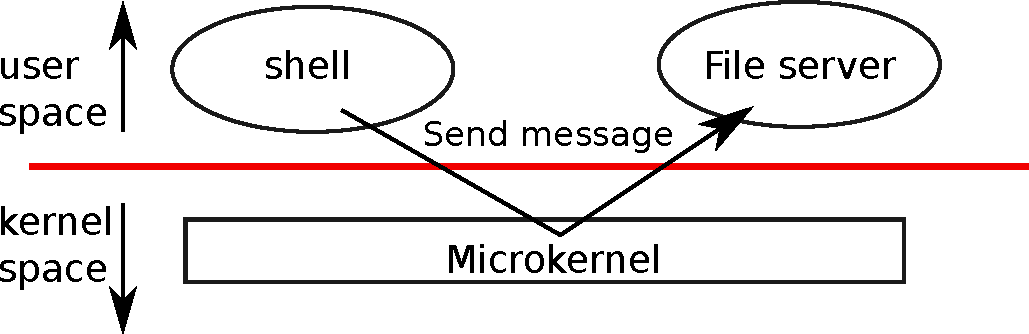
\includegraphics[scale=0.5]{fig/mkernel.pdf}
\caption{A microkernel with a file system server}
\label{fig:mkernel}
\end{figure}

Figure~\ref{fig:mkernel}
illustrates this microkernel design.  In the figure, the file system runs as a
user-level process.  OS services running as processes are called servers.
To allow applications to interact with the
file server, the kernel provides an inter-process communication
mechanism to send messages from one
user-mode process to another.  For example, if an application like the shell
wants to read or write a file, it sends a message to the file server and waits
for a response. 

In a microkernel, the kernel interface consists of a few low-level
functions for starting applications, sending messages,
accessing device hardware, etc.  This organization allows the kernel to be 
relatively simple, as most of the operating system
resides in user-level servers.

Xv6 is
implemented as a monolithic kernel, like most Unix operating systems.
Thus, the xv6 kernel interface corresponds to the operating system
interface, and the kernel implements the complete operating system.  Since 
xv6 doesn't provide many services, its kernel is smaller than some
microkernels, but conceptually xv6 is monolithic.
%% 
\section{Process overview}
%% 

The unit of isolation in xv6 (as in other Unix operating systems) is a 
\indextext{process}.
The process abstraction prevents one process from wrecking or spying on
another process's memory, CPU, file descriptors, etc.  It also prevents a process
from wrecking the kernel itself, so that a process can't subvert the kernel's
isolation mechanisms.
The kernel must implement the process abstraction with care because
a buggy or malicious application may trick the kernel or hardware in doing
something bad (e.g., circumventing isolation).  The mechanisms used by
the kernel to implement processes include the user/supervisor mode flag, address spaces,
and time-slicing of threads.

To help enforce isolation, the process abstraction provides the
illusion to a program that it has its own private machine.  A process provides
a program with what appears to be a private memory system, or
\indextext{address space}, 
which other processes cannot read or write.
A process also provides the program with what appears to be its own
CPU to execute the program's instructions.

Xv6 uses page tables (which are implemented by hardware) to give each process
its own address space. The RISC-V page table
translates (or ``maps'') a
\indextext{virtual address}
(the address that an RISC-V instruction manipulates) to a
\indextext{physical address}
(an address that the CPU chip sends to main memory).

\begin{figure}[t]
\center
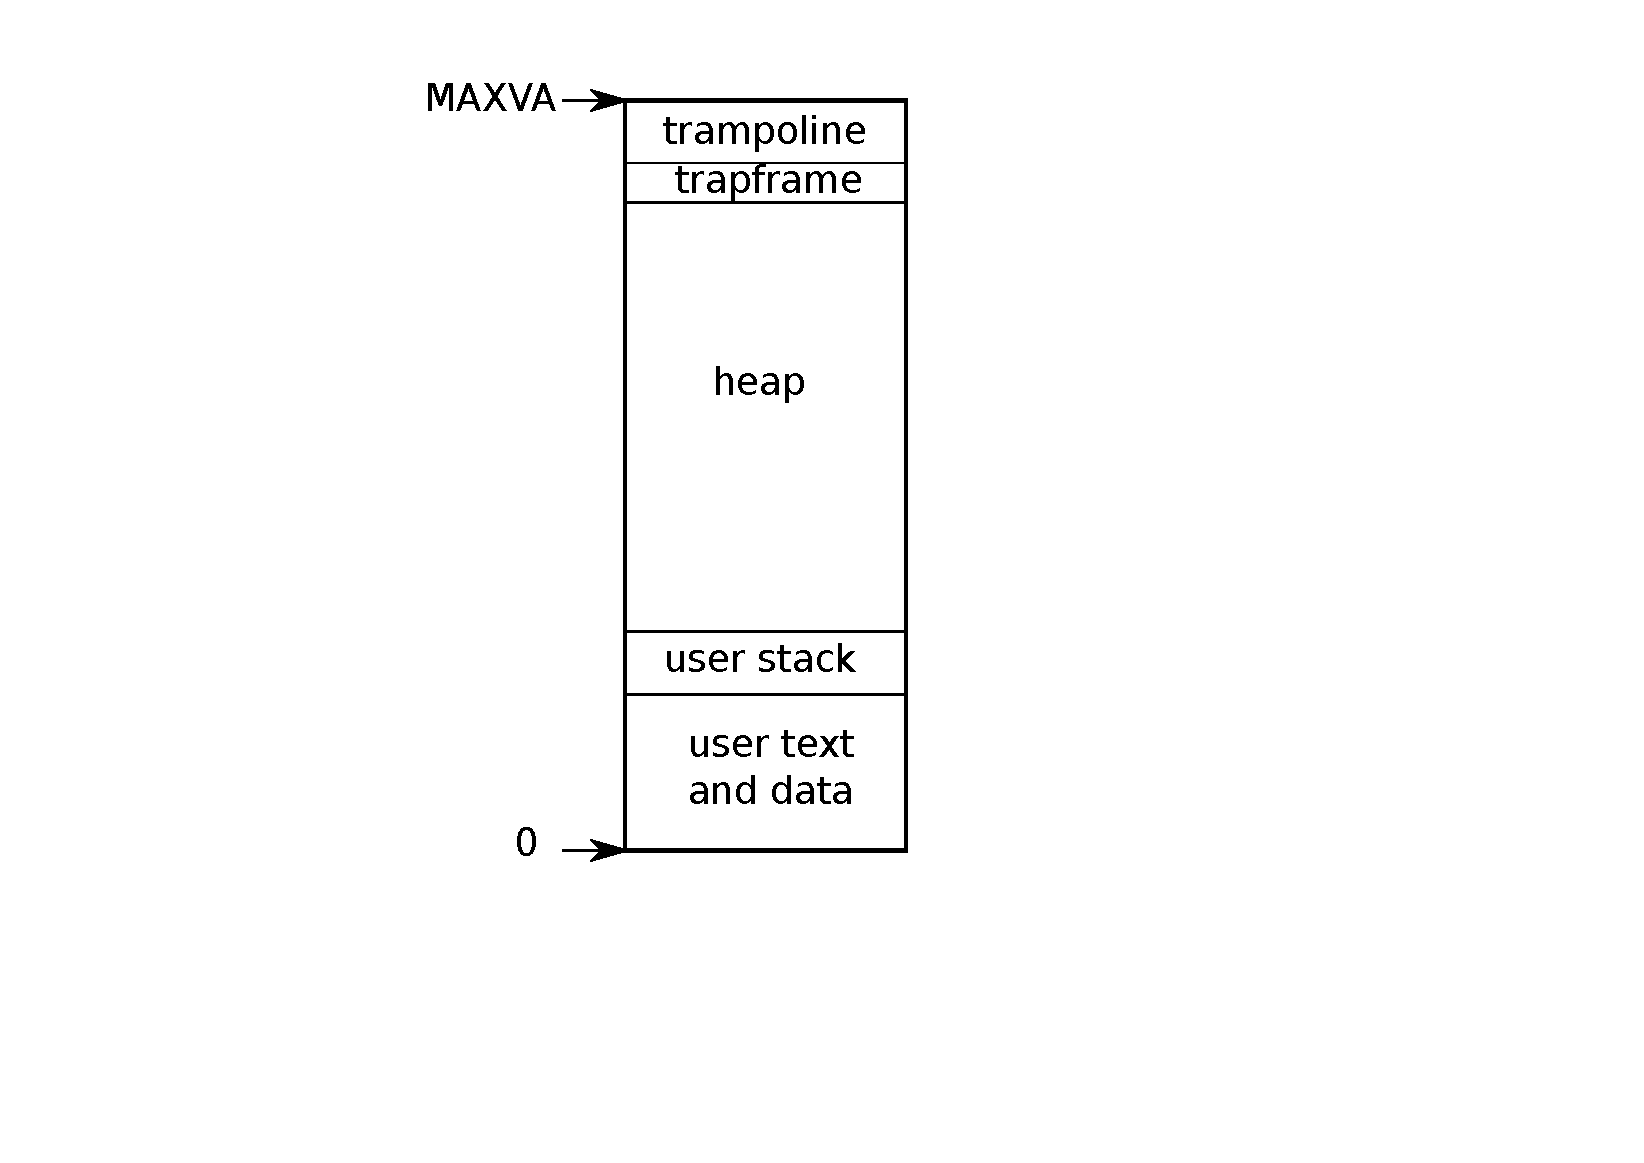
\includegraphics[scale=0.5]{fig/as.pdf}
\caption{Layout of a virtual address space of a user process}
\label{fig:as}
\end{figure}

Xv6 maintains a separate page table for each process that defines that process's
address space. As illustrated in 
Figure~\ref{fig:as},
an address space includes the process's
\indextext{user memory}
starting at virtual address zero. Instructions come first,
followed by global variables, then the stack,
and finally a ``heap'' area (for malloc)
that the process can expand as needed.
Xv6 runs on RISC-V with 39 bits for virtual addresses,
but uses only 38 bits.  Thus, the maximum address is $2^{38}-1$ =
0x3fffffffff, which is \lstinline{MAXVA}~\lineref{kernel/riscv.h:/MAXVA/}.
At the top of the address space xv6 reserves a page
for a \indextext{trampoline} and a page mapping
the process's \indextext{trapframe}
to switch to the kernel, as we will explain in Chapter~\ref{CH:TRAP}.

The xv6 kernel maintains many pieces of state for each process,
which it gathers into a
\indexcode{struct proc}
\lineref{kernel/proc.h:/^struct.proc/}.
A process's most important pieces of kernel state are its 
page table, its kernel stack, and its run state.
We'll use the notation
\indexcode{p->xxx}
to refer to elements of the
\lstinline{proc}
structure.  The trapframe mentioned above is \indexcode{p->tf}.

Each process has a thread of execution (or 
\indextext{thread}
for short) that executes the process's instructions.
A thread can be suspended and later resumed.
To switch transparently between processes,
the kernel suspends the currently running thread and resumes another process's
thread.  Much of the state of a thread (local variables, function call return
addresses) is stored on the thread's stacks.
Each process has two stacks: a user stack and a kernel stack
(\indexcode{p->kstack}).
When the process is executing user instructions, only its user stack
is in use, and its kernel stack is empty.
When the process enters the kernel (for a system call or interrupt),
the kernel code executes on the process's kernel stack; while
a process is in the kernel, its user stack still contains saved
data, but isn't actively used.
A process's thread alternates between actively using its user stack
and its kernel stack. The kernel stack is separate (and protected from
user code) so that the kernel
can execute even if a process has wrecked its user stack.

A process can make a system call by executing the RISC-V \indexcode{ecall}
instruction. This instruction raises the hardware privilege level and
changes the program counter to a kernel-defined entry point.  The code
at the entry point switches to a kernel stack and executes the kernel
instructions that implement the system call.  When the system call
completes, the kernel switches back to the user stack and returns to
user space by calling the \indexcode{sret} instruction, which lowers
the hardware privilege level and resumes executing user instructions
just after the system call instruction.  A process's thread can
``block'' in the kernel to wait for I/O, and resume where it left off
when the I/O has finished.

\indexcode{p->state} 
indicates whether the process is allocated, ready
to run, running, waiting for I/O, or exiting.

\indexcode{p->pagetable}
holds the process's page table, in the format
that the RISC-V hardware expects.
xv6 causes the paging hardware to use a process's
\lstinline{p->pagetable}
when executing that process in user space.
A process's page table also serves as the record of the
addresses of the physical pages allocated to store the process's memory.
%% 
\section{Code: starting xv6 and the first process}
%% 
To make xv6 more concrete, we'll outline how the kernel starts and
runs the first process. The subsequent chapters will describe the
mechanisms that show up in this overview in more detail.

When the RISC-V development board powers on, it initializes
itself and runs a boot loader which is stored in read-only
memory.  The boot loader loads the xv6 kernel into memory.  Then, in
machine mode, the CPU executes xv6 starting at
\indexcode{\_entry}
\lineref{kernel/entry.S:/^.entry:/}.
Xv6 starts with the RISC-V paging hardware disabled:
virtual addresses map directly to physical addresses.

The loader loads the xv6 kernel into memory at physical address
\texttt{0x80000000}.
The reason it places the kernel at
\texttt{0x80000000}
rather than
\texttt{0x0}
is because the address range
\texttt{0x0:0x80000000}
contains I/O devices.

The instructions at
\lstinline{_entry}
set up a stack so that xv6 can run C code.
xv6 declares space for an initial stack,
\lstinline{stack0},
in the file
\lstinline{start.c}
\lineref{kernel/start.c:/stack0/}.
The code at
\lstinline{_entry}
loads the stack pointer register
\texttt{sp}
with the address
\lstinline{stack0+4096},
the top of the stack, because the stack
on RISC-V grows down.
Now that we have a stack,
\lstinline{_entry}
calls into C code at
\lstinline{start}
\lineref{kernel/start.c:/^start/}.

The function
\lstinline{start}
performs some configuration that is only allowed in
machine mode, and then switches to supervisor mode.
To enter supervisor mode, RISC-V
provides the instruction
\lstinline{mret}.
This instruction is most often used to return from
a previous call from supervisor mode to machine mode.
\lstinline{start} isn't returning from such a call, and
instead sets things up as if there had been one:
it sets the previous privilege mode to
supervisor in the register
\lstinline{mstatus},
it sets the return address to
\lstinline{main}
by writing
\lstinline{main}'s
address into
the register
\lstinline{mepc},
disables virtual memory in supervisor mode
by writing
\lstinline{0}
into the page-table register
\lstinline{satp},
and delegates all interrupts and exceptions
to supervisor mode.

Before jumping into supervisor mode,
\lstinline{start}
performs one more task: it programs the clock
chip to generate timer interrupts.
With this housekeeping out of the way,
\lstinline{start}
``returns'' to supervisor
mode by calling
\lstinline{mret}.
This causes the program counter to change
to
\lstinline{main}
\lineref{kernel/main.c:/^main/}.

After
\lstinline{main}
\lineref{kernel/main.c:/^main/}  
initializes several devices and subsystems, 
it creates the first process by calling 
\lstinline{userinit}
\lineref{kernel/proc.c:/^userinit/}.
The first process executes a small program,
\indexcode{initcode.S} 
\lineref{user/initcode.S:1},
which re-enters the kernel by invoking the
\lstinline{exec}
system call.
As we saw in Chapter~\ref{CH:UNIX}, 
\indexcode{exec}
replaces the memory and registers of the
current process with a new program (in this case,
\lstinline{/init}).
Once the kernel has completed 
\lstinline{exec},
it returns to user space and runs
\indexcode{/init}.
\lstinline{Init}
\lineref{user/init.c:/^main/}
creates a new console device file
if needed
and then opens it as file descriptors 0, 1, and 2.
Then it loops,
starting a console shell, 
handles orphaned zombies until the shell exits,
and repeats.
The system is up.
%% 
\section{Real world}
%% 

In the real world, one can find both monolithic kernels and microkernels. Many
Unix kernels are monolithic. For example, Linux has a monolithic kernel,
although some OS functions run as user-level servers (e.g., the windowing
system).  Kernels such as L4, Minix, QNX are organized as a microkernel with
servers, and have seen wide deployment in embedded settings.

Most operating systems have adopted the process concept, and most
processes look similar to xv6's.  Modern operating systems, however,
support several threads within a process, to allow a single process to
exploit multiple CPUs.  Supporting multiple threads in a
process involves quite a bit of machinery that xv6 doesn't have,
including potential interface changes (e.g., Linux's
\lstinline{clone},
a variant of
\lstinline{fork}),
to control which parts of
a process threads share.
%% 
\section{Exercises}
%%

\begin{enumerate}
  
\item Set a breakpoint at \lstinline{swtch}.  Single step with gdb's
\lstinline{stepi}
through the ret to
\lstinline{forkret},
then use gdb's
\lstinline{finish}
to proceed to
\lstinline{usertrapret},
then
\lstinline{stepi}
until you get to
\lstinline{initcode} 
at virtual address zero.

\end{enumerate}

% talk a little about initial page table conditions:
%     paging not on, but virtual mostly mapped direct to physical,
%     which is what things look like when we turn paging on as well
%     since paging is turned on after we create first process.
%   mention why still have SEG_UCODE/SEG_UDATA?
%   do we ever really say what the low two bits of %cs do?
%     in particular their interaction with PTE_U
%   sidebar about why it is extern char[]
\chapter{Page tables}
\label{CH:MEM}

Page tables are the mechanism through which the operating system
provides each process with its own private memory.  Page tables
determinate what memory addresses mean.  They allow xv6 to multiplex
the address spaces of different processes onto a single physical
memory, and to protect the memories of different processes.  The level
of indirection provided by page tables also allows many neat tricks.

xv6 uses page tables primarily to multiplex address spaces and to
protect memory.  It also uses a few simple page-table tricks: mapping
the same memory (a trampoline page) in several address spaces, and
guarding a user stack with an unmapped page.  The rest of this chapter
explains the page tables that the RISC-V hardware provides and how xv6
uses them.  Compared to a real-world operating system, xv6's design is
restrictive, but it does illustrate the key ideas.
%% 
\section{Paging hardware}
%% 
As a reminder,
RISC-V instructions (both user and kernel) manipulate virtual addresses.
The machine's RAM, or physical memory, is indexed with physical
addresses.
The RISC-V page table hardware connects these two kinds of addresses,
by mapping each virtual address to a physical address.

xv6 runs on Sv39 RISC-V processor with has 39-bit virtual addresses;
the top of 25 bits of a 64-bit virtual address are unused.  In this
configuration, a RISC-V page table is logically an array of $2^{27}$
(134,217,728)
\textit{page table entries (PTEs)}\index{page table entries (PTEs)}.
Each PTE contains a
44-bit physical page number (PPN) and some flags. The paging
hardware translates a virtual address by using the top 27 bits
of the 39 bits to index into the page table to find a PTE, and
making a 56-bit physical address by setting
the address's top 44 bits with the PPN in the PTE.  The paging hardware
copies the low 12 bits unchanged from the virtual to the
translated physical address.  Thus a page table gives
the operating system control over virtual-to-physical address translations
at the granularity of aligned chunks of 4096 ($2^{12}$) bytes.
Such a chunk is called a
\textit{page}\index{page}.

\begin{figure}[t]
\center
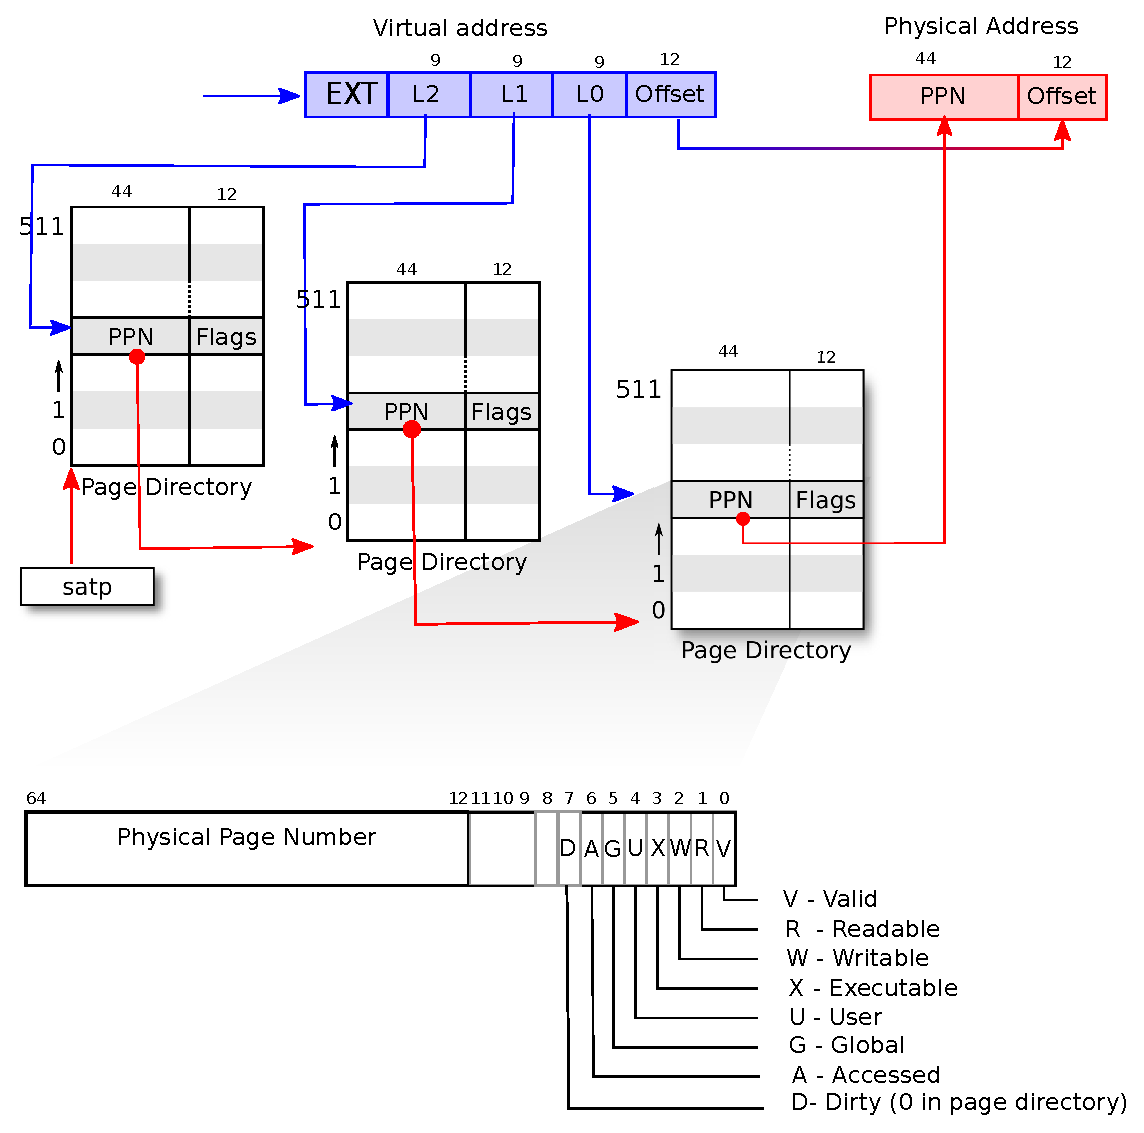
\includegraphics[scale=0.5]{fig/riscv_pagetable.eps}
\caption{RISC-V page table hardware.}
\label{fig:riscv_pagetable}
\end{figure}

As shown in
Figure~\ref{fig:riscv_pagetable},
the actual translation happens in three steps.  A page table is stored
in physical memory as a three-level tree.
The root of the tree is a
4096-byte page that contains 512 PTEs, which contains the physical
addresses for pages for the next level in the tree.  Each one of those
pages contains 512 PTEs for the final level in the tree.  The paging
hardware uses the top 9 bits of the 27 bits to select a PTE in the
root page, the middle 9 bits to select a PTE in next level of the
tree, and the bottom 9 bits to select the final PTE.

If any of the PTEs is not present, the paging hardware raises a fault.
This three-level structure allows a page table to omit entire page
table pages in the common case in which large ranges of virtual
addresses have no mappings.

In Sv39 RISC-V processors, the top 25 bits of virtual address are not
used for translation; in the future, RISC-V can use those bits to
define more levels of translation.  Similarly, the physical address
has room for growth; in Sv39 it is 56 bits, but could grow to 64 bits.

Each PTE contains flag bits that tell the paging hardware
how the associated virtual address is allowed to be used.
\indexcode{PTE_V}
indicates whether the PTE is present: if it is
not set, a reference to the page causes a fault (i.e. is not allowed).
\indexcode{PTE_R}
controls whether instructions are allowed to issue
reads to the page.
\indexcode{PTE_W}
controls whether instructions are allowed to issue
writes to the page.
\indexcode{PTE_X}
controls whether the processor may interpret the content
of the page as instruction and execute them.
Figure~\ref{fig:riscv_pagetable}
shows how it all works.
The flags and all other page hardware related structures are defined in
\fileref{kernel/riscv.h}

To tell the hardware to use a page table, the kernel must
write the physical address of the root page into the register
\texttt{\%satp}\index{satp@\lstinline{satp}}.
Each processor has its own
\texttt{\%satp}.
A processor will translate all addresses in subsequent instructions
using its page table.
Each processor has its own page-table register so that one processor
can run one process concurrently with another processor running
another process, with their memories isolated from each other.

A few notes about terms.
Physical memory refers to storage cells in DRAM.
A byte of physical memory has an address, called a physical address.
Instructions use only virtual addresses, which the
paging hardware translates to physical addresses, and then
sends to the DRAM hardware to read or write storage.
At this level of discussion there is no such thing as virtual memory,
only virtual addresses.

\begin{figure}[t]
\center
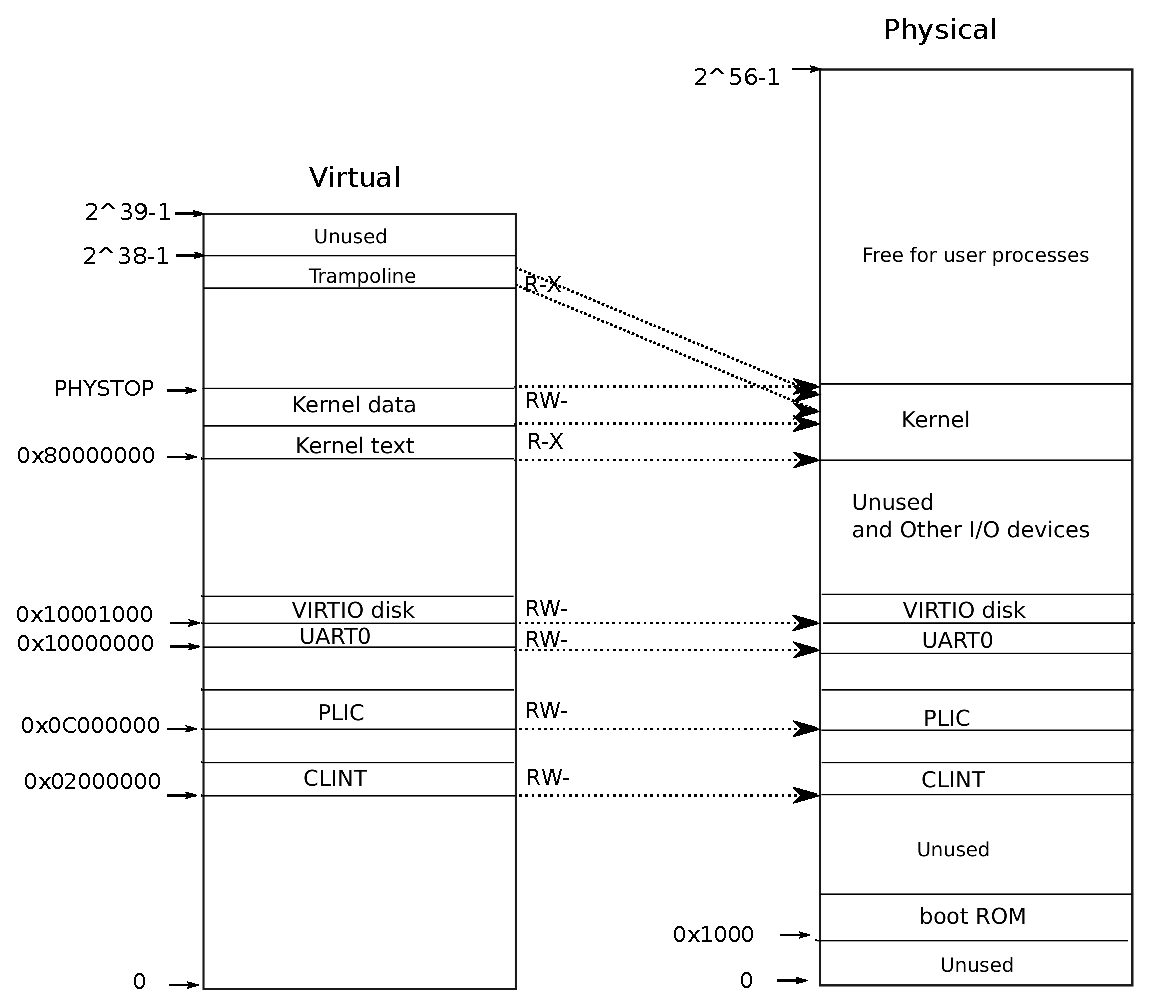
\includegraphics[scale=0.5]{fig/xv6_layout.eps}
\caption{Layout of the kernel address space.}
\label{fig:xv6_layout}
\end{figure}
%% 
\section{Kernel address space}
%% 
The kernel has its own page table.  When a process enters kernel
space, xv6 switches to the kernel page table, and when the kernel
returns to user space, it switches to the page table of the user
process.  The memory of the kernel is private.

Figure~\ref{fig:xv6_layout}
shows the layout of the kernel address space, and the mapping from
virtual addresses to physical addresses.  The file
\fileref{kernel/memlayout.h}
declares the constants for xv6's kernel memory layout.

The RISC-V development board has a number of
\textit{memory-mapped}\index{memory-mapped}
devices that sit below
\texttt{0x80000000}
in physical memory. The particular addresses are chosen by the board's
manufacturer.  The kernel can interact with devices by reading/writing
memory locations, and the board routes those reads and writes to the
appropriate devices. For example, as we saw in Chapter~\ref{CH:FIRST}, the kernel
programmed the CLINT to generate clock interrupts.  We will
see later how xv6 interacts with the other devices.

The kernel uses an identity mapping for most virtual addresses.  For,
example, the kernel itself is located at
\lstinline{KERNBASE}
in the virtual address space and in physical memory.  Same for all
devices.  The one exception is the page holding trampoline code, which
is mapped at the top of virtual address space; user page tables have
this same mapping.  In chapter~\ref{CH:TRAP}, we will discuss the role
of the trampoline page, but we see here an interesting use case of
page tables; a physical page (holding the trampoline code) is
mapped twice in the virtual address space of the kernel: once at top
of the virtual address space and once in the kernel text.

The kernel maps the pages for the trampoline and the kernel text with
the permissions
\lstinline{PTE_R}
and
\lstinline{PTE_X}.
The kernel reads and executes instructions from these pages.
The kernel maps the other pages with the permissions
\lstinline{PTE_R}
and
\lstinline{PTE_W},
so that it read and write the memory in those pages.
%% 
\section{Process address space}
%% 

Each process has a separate page table, and when xv6 switches between
processes, xv6 also changes page tables.
As shown in
Figure~\ref{fig:as},
a process's user memory starts at virtual address
zero and can grow up to
\texttt{MAXVA}
\lineref{kernel/riscv.h:/MAXVA/},
allowing a process to address in principle 256 Gigabyte of memory.

When a process asks xv6 for more memory,
xv6 first finds free physical pages in the area
labeled "Free memory", the area above the end of the data segment
of the kernel and below
\texttt{PHYSTOP}.
It then adds PTEs to the process's page table that point
to the new physical pages.
xv6 sets the
\lstinline{PTE_W},
\lstinline{PTE_X},
\lstinline{PTE_R},
\lstinline{PTE_U},
and
\lstinline{PTE_V}
flags in these PTEs.
Most processes do not use the entire user address space;
xv6 leaves
\lstinline{PTE_V}
clear in unused PTEs.

We see here a few nice examples of use of page tables.  First,
different processes' page tables translate user addresses to different
pages of physical memory, so that each process has private user
memory.  Second, each process sees its memory as having contiguous
virtual addresses starting at zero, while the process's physical
memory can be non-contiguous.  Third, the kernel maps the page with
trampoline code also at the top of address space of user processes,
thus a single page of physical memory shows up in all address spaces.
%% 
\section{Code: creating an address space}
%% 

\indexcode{main}
calls
\indexcode{kvminit}
\lineref{kernel/vm.c:/^kvminit/}
to create the kernel page table.
\lstinline{Kvminit}
first allocates a page of memory to hold the page directory.
Then it calls
\indexcode{mappages}
to install the translations that the kernel needs.
The translations include the kernel's
instructions and data, physical memory up to
\indexcode{PHYSTOP},
and memory ranges which are actually devices.

\indexcode{mappages}
\lineref{kernel/vm.c:/^mappages/}
installs mappings into a page table
for a range of virtual addresses to
a corresponding range of physical addresses.
It does this separately for each virtual address in the range,
at page intervals.
For each virtual address to be mapped,
\lstinline{mappages}
calls
\indexcode{walk}
to find the address of the PTE for that address.
It then initializes the PTE to hold the relevant physical page
number, the desired permissions (e.g.,
\lstinline{PTE_W}
\lstinline{PTE_X},
and/or
\lstinline{PTE_R}),
and
\lstinline{PTE_V}
to mark the PTE as valid
\lineref{kernel/vm.c:/perm...PTE_V/}.

\indexcode{walk}
\lineref{kernel/vm.c:/^walk/}
mimics the actions of the RISC-V paging hardware as it
looks up the PTE for a virtual address (see
Figure~\ref{fig:riscv_pagetable}).
\lstinline{walk}
traverses the 3-level page table down 9 bits at the time.
It uses the level's 9 bits of the virtual address to find
the PTE
\lineref{kernel/vm.c:/pte.=..pagetable/}.
If the PTE isn't valid, then
the required page hasn't yet been allocated;
if the
\lstinline{alloc}
argument is set,
\lstinline{walk}
allocates it and puts its physical address in the PTE.
It returns the PTE in lowest layer in the tree
\lineref{kernel/vm.c:/return..pagetable/}.

\indexcode{main}
calls
\indexcode{kvminithart}
\lineref{kernel/vm.c:/^kvminithart/}
to install the kernel page table.
It writes the physical address of the root page
into the register
\texttt{\%satp}.
After this the processor will translate addresses using the kernel
page table.  Since the kernel uses an identity mapping, the now
virtual address of the next instruction will map to the right physical
memory address.
%% 
\section{Physical memory allocation}
%% 

The kernel must allocate and free physical memory at run-time for
page tables,
process user memory,
kernel stacks,
and pipe buffers.

xv6 uses the physical memory between the end of the kernel and
\indexcode{PHYSTOP}
for run-time allocation. It allocates and frees whole 4096-byte pages
at a time. It keeps track of which pages are free by threading a
linked list through the pages themselves. Allocation consists of
removing a page from the linked list; freeing consists of adding the
freed page to the list.
%% 
\section{Code: Physical memory allocator}
%% 

The allocator's data structure is a
\textit{free list}
of physical memory pages that are available
for allocation.
Each free page's list element is a
\indexcode{struct run}
\lineref{kernel/kalloc.c:/^struct.run/}.
Where does the allocator get the memory
to hold that data structure?
It store each free page's
\lstinline{run}
structure in the free page itself,
since there's nothing else stored there.
The free list is
protected by a spin lock
\linerefs{kernel/kalloc.c:/^struct.{/,/}/}.
The list and the lock are wrapped in a struct
to make clear that the lock protects the fields
in the struct.
For now, ignore the lock and the calls to
\lstinline{acquire}
and
\lstinline{release};
Chapter~\ref{CH:LOCK} will examine
locking in detail.

The function
\indexcode{main}
calls
\indexcode{kinit}
to initialize the allocator
\lineref{kernel/kalloc.c:/^kinit/}.
\lstinline{kinit}
enables locking and arranges for more memory to be allocatable.
\lstinline{main}
ought to determine how much physical
memory is available by parsing configuration information.
Instead xv6 assumes that the machine has
224 megabytes
(\lstinline{PHYSTOP})
of physical memory, and uses all the memory between the end of the kernel
and
\indexcode{PHYSTOP}
as the initial pool of free memory.
\lstinline{kinit}
calls
\indexcode{freerange}
to add memory to the free list via per-page calls to
\indexcode{kfree}.
A PTE can only refer to a physical address that is aligned
on a 4096-byte boundary (is a multiple of 4096), so
\lstinline{freerange}
uses
\indexcode{PGROUNDUP}
to ensure that it frees only aligned physical addresses.
The allocator starts with no memory;
these calls to
\lstinline{kfree}
give it some to manage.

The allocator sometimes treats addresses as integers
in order to perform arithmetic on them (e.g.,
traversing all pages in
\lstinline{kinit}),
and sometimes uses addresses as pointers to read and
write memory (e.g., manipulating the
\lstinline{run}
structure stored in each page);
this dual use of addresses is the main reason that the
allocator code is full of C type casts.
\index{type cast}
The other reason is that freeing and allocation inherently
change the type of the memory.

The function
\lstinline{kfree}
\lineref{kernel/kalloc.c:/^kfree/}
begins by setting every byte in the
memory being freed to the value 1.
This will cause code that uses memory after freeing it
(uses ``dangling references'')
to read garbage instead of the old valid contents;
hopefully that will cause such code to break faster.
Then
\lstinline{kfree}
casts
\lstinline{v}
to a pointer to
\lstinline{struct}
\lstinline{run},
records the old start of the free list in
\lstinline{r->next},
and sets the free list equal to
\lstinline{r}.
\indexcode{kalloc}
removes and returns the first element in the free list.
%% 
\section{User part of an address space}
%% 

\begin{figure}[t]
\center
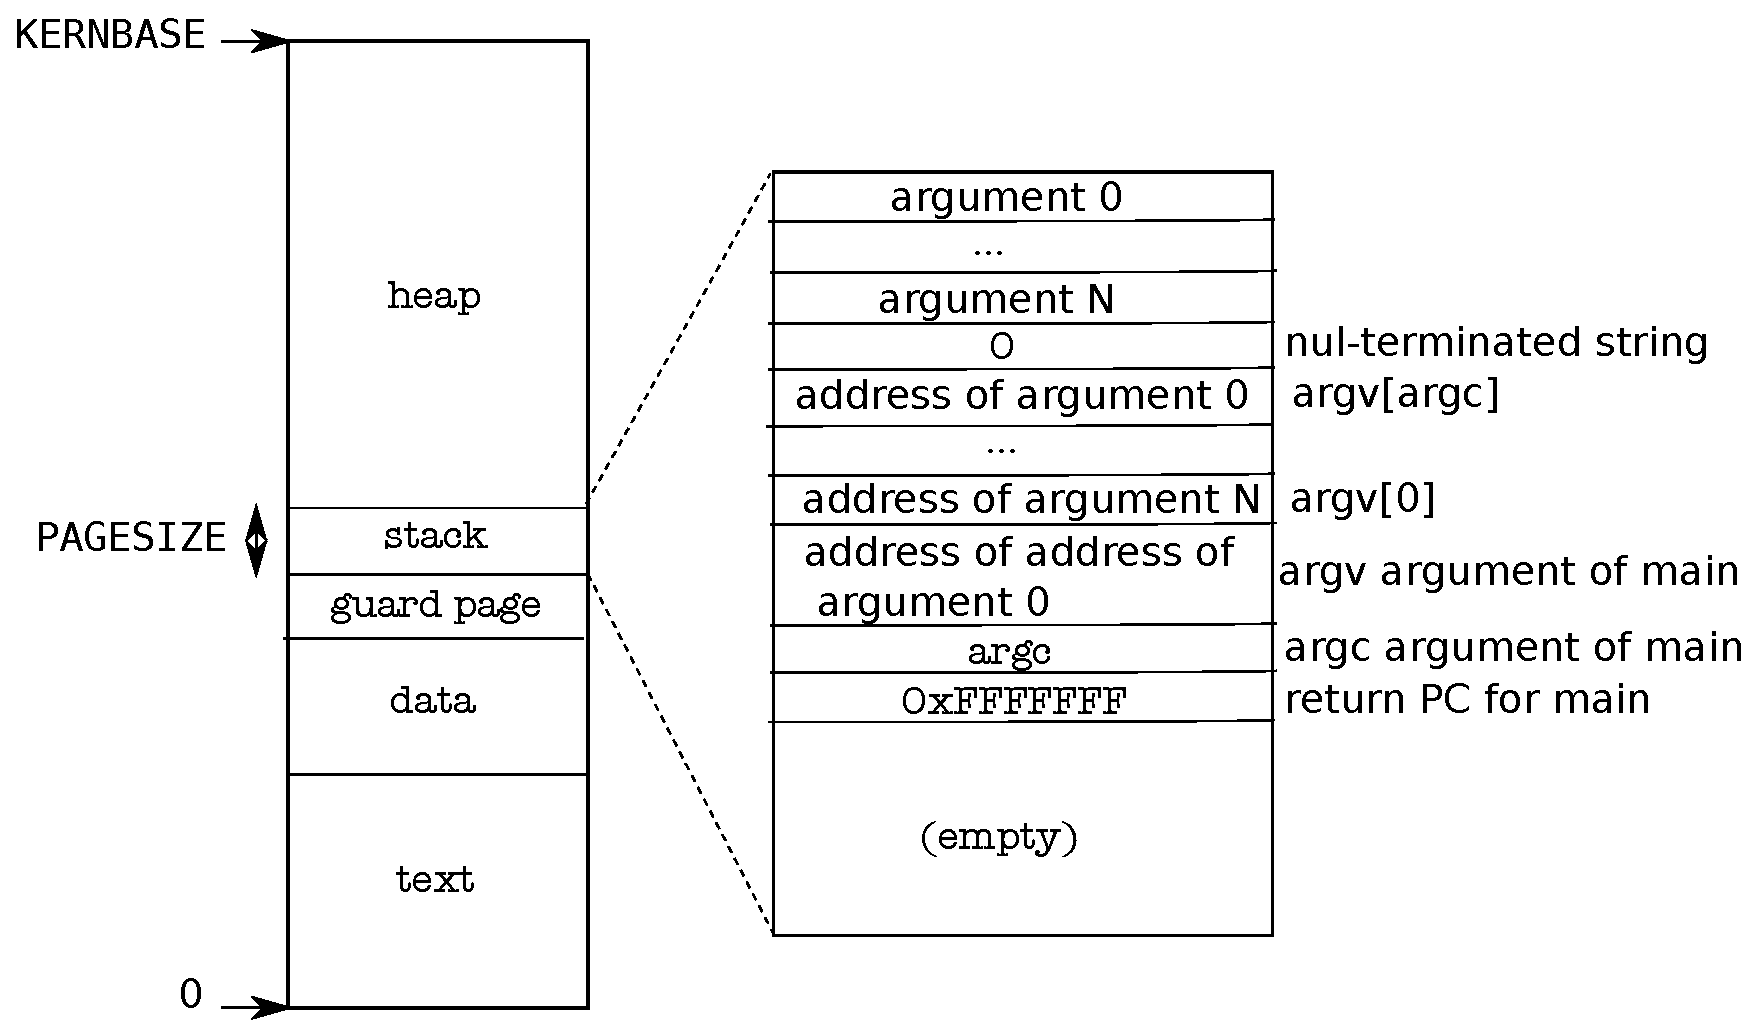
\includegraphics[scale=0.5]{fig/processlayout.eps}
\caption{Memory layout of a user process with its initial stack.}
\label{fig:processlayout}
\end{figure}

Figure~\ref{fig:processlayout}
shows the layout of the user memory of an executing process in xv6.
Each user process starts at address 0. The bottom of the address space
contains the text for the user program, its data, and its stack.
The heap is above the stack so that the heap can expand when the process
calls
\indexcode{sbrk}.
Note that the text, data, and stack sections are layed out contiguously in the
process's address space but xv6 is free to use non-contiguous physical pages for
those sections. For example, when xv6 expands a process's heap, it can use any
free physical page for the new virtual page and then program the page table
hardware to map the virtual page to the allocated physical page.  This
flexibility is a major advantage of using paging hardware.

The stack is a single page, and is
shown with the initial contents as created by exec.
Strings containing the command-line arguments, as well as an
array of pointers to them, are at the very top of the stack.
Just under that are values that allow a program
to start at
\lstinline{main}
as if the function call
\lstinline{main(argc},
\lstinline{argv)}
had just started.
To guard a stack growing off the stack page, xv6 places a guard page right below
the stack.  The guard page is not mapped and so if the stack runs off the stack
page, the hardware will generate an exception because it cannot translate the
faulting address.
A real-world operating system might allocate more space for the stack so that it can
grow beyond one page.
%% 
\section{Code: sbrk}
%% 
\lstinline{Sbrk}
is the system call for a process to shrink or grow its memory. The system
call is implemented by the function
\lstinline{growproc}
\lineref{kernel/proc.c:/^growproc/}.
If
\lstinline{n}
is postive,
\lstinline{growproc}
allocates one or more physical pages and maps them at the top of the process's
address space.  If
\lstinline{n}
is negative,
\lstinline{growproc}
unmaps one or more pages from the process's address space and frees the corresponding
physical pages.
To make these changes,
xv6 modifies the process's page table.  The process's page table is stored in
memory, and so the kernel can update the table with ordinary assignment
statements, which is what
\lstinline{allocuvm}
and
\lstinline{deallocuvm}
do.

The RISC-V hardware caches page table entries in a
\textit{Translation Look-aside Buffer (TLB)}\index{Translation Look-aside Buffer (TLB)},
and when xv6 changes the page tables, it must invalidate the cached entries.  If
it didn't invalidate the cached entries, then at some point later the TLB might
use an old mapping, pointing to a physical page that in the mean time has been
allocated to another process, and as a result, a process might be able to
scribble on some other process's memory.  Reloading the register
\texttt{\%satp}
will flush the TLB, and xv6 reloads this register
when the kernel returns to user space to switch to the user process's
page table.
%% 
\section{Code: exec}
%% 
\lstinline{Exec}
is the system call that creates the user part of an address space.  It
initializes the user part of an address space from a file stored in the file
system.
\lstinline{Exec}
\lineref{kernel/exec.c:/^exec/}
opens the named binary
\lstinline{path}
using
\indexcode{namei}
\lineref{kernel/exec.c:/namei/},
which is explained in Chapter~\ref{CH:FS}.
Then, it reads the ELF header. Xv6 applications are described in the widely-used
\textit{ELF format}\index{ELF format},
defined in
\fileref{kernel/elf.h}.
An ELF binary consists of an ELF header,
\indexcode{struct elfhdr}
\lineref{kernel/elf.h:/^struct.elfhdr/},
followed by a sequence of program section headers,
\lstinline{struct proghdr}
\lineref{kernel/elf.h:/^struct.proghdr/}.
Each
\lstinline{proghdr}
describes a section of the application that must be loaded into memory;
xv6 programs have only one program section header, but
other systems might have separate sections
for instructions and data.

The first step is a quick check that the file probably contains an
ELF binary.
An ELF binary starts with the four-byte ``magic number''
\lstinline{0x7F},
.code 'E',
.code 'L',
.code 'F',
or
\indexcode{ELF_MAGIC}
\lineref{kernel/elf.h:/ELF_MAGIC/}.
If the ELF header has the right magic number,
\lstinline{exec}
assumes that the binary is well-formed.

\lstinline{Exec}
allocates a new page table with no user mappings with
\indexcode{proc_pagetable}
\lineref{kernel/exec.c:/proc_pagetable/},
allocates memory for each ELF segment with
\indexcode{uvmalloc}
\lineref{kernel/exec.c:/uvmalloc/},
and loads each segment into memory with
\indexcode{loadseg}
\lineref{kernel/exec.c:/loadseg/}.
\lstinline{loadseg}
uses
\indexcode{walkaddr}
to find the physical address of the allocated memory at which to write
each page of the ELF segment, and
\indexcode{readi}
to read from the file.

The program section header for
\indexcode{/init},
the first user program created with
\lstinline{exec},
looks like this:
\begin{lstlisting}[]
# objdump -p _init
user/_init:     file format elf64-littleriscv

Program Header:
    LOAD off    0x00000000000000b0 vaddr 0x0000000000000000 paddr 0x0000000000000000 align 2**3
         filesz 0x0000000000000840 memsz 0x0000000000000858 flags rwx
   STACK off    0x0000000000000000 vaddr 0x0000000000000000 paddr 0x0000000000000000 align 2**4
         filesz 0x0000000000000000 memsz 0x0000000000000000 flags rw-
\end{lstlisting}

The program section header's
\lstinline{filesz}
may be less than the
\lstinline{memsz},
indicating that the gap between them should be filled
with zeroes (for C global variables) rather than read from the file.
For
\lstinline{/init},
\lstinline{filesz}
is 2112 bytes and
\lstinline{memsz}
is 2136 bytes,
and thus
\indexcode{uvmalloc}
allocates enough physical memory to hold 2136 bytes, but reads only 2112 bytes
from the file
\lstinline{/init}.

Now
\indexcode{exec}
allocates and initializes the user stack.
It allocates just one stack page.
\lstinline{Exec}
copies the argument strings to the top of the stack
one at a time, recording the pointers to them in
\indexcode{ustack}.
It places a null pointer at the end of what will be the
\indexcode{argv}
list passed to
\lstinline{main}.
The first three entries in
\lstinline{ustack}
are the fake return PC,
\indexcode{argc},
and
\lstinline{argv}
pointer.

\lstinline{Exec}
places an inaccessible page just below the stack page,
so that programs that try to use more than one page will fault.
This inaccessible page also allows
\lstinline{exec}
to deal with arguments that are too large;
in that situation,
the
\indexcode{copyout}
\lineref{kernel/vm.c:/^copyout/}
function that
\lstinline{exec}
uses to copy arguments to the stack will notice that
the destination page is not accessible, and will
return \-1.

During the preparation of the new memory image,
if
\lstinline{exec}
detects an error like an invalid program segment,
it jumps to the label
\lstinline{bad},
frees the new image,
and returns \-1.
\lstinline{Exec}
must wait to free the old image until it
is sure that the system call will succeed:
if the old image is gone,
the system call cannot return \-1 to it.
The only error cases in
\lstinline{exec}
happen during the creation of the image.
Once the image is complete,
\lstinline{exec}
can commit to the new page table
\lineref{kernel/exec.c:/pagetable.=.pagetable/}
and free the old one
\lineref{kernel/exec.c:/proc_freepagetable/}.

\lstinline{Exec}
loads bytes from the ELF file into memory at addresses specified by the ELF file.
Users or processes can place whatever addresses they want into an ELF file.
Thus
\lstinline{exec}
is risky, because the addresses in the ELF file may refer to the kernel, accidentally
or on purpose. The consequences for an unwary kernel could range from
a crash to a malicious subversion of the kernel's isolation mechanisms
(i.e., a security exploit).
xv6 performs a number of checks to avoid these risks.
For example
\lstinline{if(ph.vaddr + ph.memsz < ph.vaddr)}
checks for whether the sum overflows a 64-bit integer.
The danger is that a user could construct an ELF binary with a
\lstinline{ph.vaddr}
that points to a user-chosen address,
and
\lstinline{ph.memsz}
large enough that the sum overflows to 0x1000, which will look like a
valid value. In an older version of xv6 in which the user address
space also contained the kernel (but not readable/writable in user
mode), the user could choose an address that corresponded to kernel
memory and would thus copy data from the ELF binary into the kernel.
In the RISC-V version of xv6 this cannot happen, because the kernel has
its own separate page table;
\lstinline{loadseg}
loads into the process's page table, not in the kernel's page table.

It is easy for a kernel developer to omit a crucial check, and
real-world kernels have a long history of missing checks whose absence
can be exploited by user programs to obtain kernel privileges.  It is likely that xv6 doesn't do a complete job of validating
user-level data supplied to the kernel, which a malicious user program might be able to exploit to circumvent xv6's isolation.
%% 
\section{Real world}
%% 

Like most operating systems, xv6 uses the paging hardware
for memory protection and mapping.
Most operating systems make far more sophisticated
use of paging than xv6; for example, xv6 lacks demand
paging from disk, copy-on-write fork, shared memory,
lazily-allocated pages,
and automatically extending stacks.

The RISC-V support physical memory protection, but xv6 doesn't use it.

On machines with lots of memory
it might make sense to use
RISC-V's support for ``super pages.''
Small pages make sense
when physical memory is small, to allow allocation and page-out to disk
with fine granularity.
For example, if a program
uses only 8 kilobytes of memory, giving it a 4 megabytes physical page is wasteful.
Larger pages make sense on machines with lots of RAM,
and may reduce overhead for page-table manipulation.

Memory allocation was a hot topic a long time ago, the basic problems being
efficient use of limited memory and
preparing for unknown future requests;
see Knuth.  Today people care more about speed than
space-efficiency.  In addition, a more elaborate kernel
would likely allocate many different sizes of small blocks,
rather than (as in xv6) just 4096-byte blocks;
a real kernel
allocator would need to handle small allocations as well as large
ones.
%% 
\section{Exercises}
%% 

\begin{enumerate}
  
\item Parse RISC-V's device tree to find the amount of physical memory
the computer has.

\item Write a user program that grows its address space with 1 byte by calling
\lstinline{sbrk(1)}.
Run the  program and investigate the page table for the program before the call
to
\lstinline{sbrk}
and after the call to
\lstinline{sbrk}.
How much space has the kernel allocated?  What does the
\lstinline{pte}
for the new memory contain?

\item Modify xv6 to use super pages for the kernel.

\item Modify xv6 so that when a user program dereferences a null pointer, it will
receive a fault.  That is, modify xv6 so that virtual address 0 isn't mapped for
user programs.

\item Unix implementations of
\lstinline{exec}
traditionally include special handling for shell scripts.
If the file to execute begins with the text
\lstinline{#!},
then the first line is taken to be a program
to run to interpret the file.
For example, if
\lstinline{exec}
is called to run
\lstinline{myprog}
\lstinline{arg1}
and
\lstinline{myprog} 's
first line is
\lstinline{#!/interp},
then
\lstinline{exec}
runs
\lstinline{/interp}
with command line
\lstinline{/interp}
\lstinline{myprog}
\lstinline{arg1}.
Implement support for this convention in xv6.

\end{enumerate}


%    Sidebar about panic:
% 	panic is the kernel's last resort: the impossible has happened and the
% 	kernel does not know how to proceed.  In xv6, panic does ...
\chapter{Traps and device drivers}
\label{CH:TRAP}

There are three situations in which some event causes the CPU to set
aside its ordinary sequential execution of instructions and forces a
transfer of control to special code that handles the event. One
situation is a system call, when a user program 
executes the {\tt ecall} instruction to ask the kernel to do 
something for it. Another situation is an \indextext{exception}:
an instruction (user or kernel) does something illegal, such as divide
by zero or use an invalid virtual address. The third situation is a
device \indextext{interrupt}, when a device signals that it needs
attention, for example when the disk hardware finishes a read or write
request.

This book uses \indextext{trap} as a generic term for these
situations. Typically whatever code was executing at the time of the
trap will later need to resume, and shouldn't need to be aware that
anything special happened. That is, we often want traps to be
transparent; this is particularly important for interrupts, which the
interrupted code typically doesn't expect. Thus the usual sequence is that
a trap forces a transfer of control into the kernel; the kernel saves
registers and other state so that execution can be resumed; the kernel
executes appropriate handler code (e.g. a system call implementation
or device driver); the kernel restores the saved state and returns
from the trap; and the original code resumes where it left off.

The xv6 kernel handles all traps. This is natural for system calls; it
makes sense for interrupts since isolation demands that user processes
not directly use devices, and because only the kernel has the state
needed for device handling; and it makes sense for exceptions since
xv6 responds to all exceptions from user space by killing the
offending program.

Xv6 trap handling proceeds in four stages: hardware actions taken by
the RISC-V CPU, an assembly ``vector'' that prepares the way for
kernel C code, a C trap handler that decides what to do with the trap,
and the system call or device driver service routine. While
commonality among the three trap types suggests that a kernel could
handle all traps with a single code path, it turns out to be
convenient to have separate assembly vectors and C trap handlers for
three distinct cases: traps from kernel space, traps from user space,
and timer interrupts.

This chapter ends with a discussion of device drivers. Device handling
is a different topic than traps, but is included here because the
kernel's interaction with device hardware is often driven by
interrupts.

\section{RISC-V trap machinery}

RISC-V supports a number of control registers that the kernel writes to
tell the CPU how to handle interrupts, and that the kernel can read
to find out about an interrupt that has occured. The RISC-V documents
contain the full story~\cite{riscv:priv}. {\tt riscv.h}
\lineref{kernel/riscv.h:1} contains definitions that xv6 uses. Here's
an outline of the most important registers:

\begin{itemize}

\item {\bf stvec}: The kernel writes the address of its trap handler
  here; the RISC-V jumps here to handle a trap.

\item {\bf sepc}: When a trap occurs, RISC-V saves the program counter
  here (since the {\tt pc} is then replaced with {\tt stvec}). The
  {\tt sret} (return from trap) instruction copies {\tt sepc} to the
  {\tt pc}. The kernel can write to {\tt sepc} to control where {\tt
    sret} goes.

\item {\bf scause}: The RISC-V puts a number here that describes
the reason for the trap.

\item {\bf sscratch}: The kernel places a value here that comes in
  handy at the very start of a trap handler.

\item {\bf sstatus}: The SIE bit controls whether device interrupts
  are enabled. If the kernel clears SIE, the RISC-V will defer
  device interrupts until the kernel sets SIE. The SPP bit
  indicates whether a trap came from user mode or supervisor
  mode, and controls to what mode {\tt sret} returns.

\end{itemize}

The above relate to interrupts handled in supervisor mode, and they
cannot be read or written in user mode. There is an equivalent set of
control registers for interrupts handled in machine mode; xv6 uses
them only for the special case of timer interrupts.

When it needs to force a trap, the RISC-V hardware does the
following for all trap types (other than timer interrupts):

\begin{enumerate}

\item If the trap is a device interrupt, and the {\tt sstatus} SIE bit
  is clear, don't do any of the following.

\item Disable interrupts by clearing SIE.

\item Copy the {\tt pc} to {\tt sepc}.

\item Save the current mode (user or supervisor) in the SPP bit in {\tt sstatus}.

\item Set {\tt scause} to reflect the interrupt's cause.

\item Set the mode to supervisor.

\item Copy {\tt stvec} to the {\tt pc}.

\item Start executing at the new {\tt pc}.

\end{enumerate}

It is important that the CPU performs all these steps as
a single operation.
Consider if one of these steps were omitted: for example, the CPU
didn't switch program counters. Then, a trap could switch to
supervisor mode while still running user instructions. Those user
instructions could break the user/kernel isolation, for example by
modifying the {\tt satp} register to point to a page table that
allowed accessing all of physical memory. It is thus important that
the kernel specify the trap entry point, and not the user program.

Note that the CPU doesn't switch to the kernel page table, doesn't
switch to a stack in the kernel, and doesn't save any registers other
than the {\tt pc}. The kernel must perform these tasks if necessary.
One reason that the CPU does minimal work during a trap is to provide
flexibility to software; for example, in some situations no page table
switch is needed, which may increase performance.

\section{Traps from kernel space}

When the xv6 kernel is executing on a CPU, two types of traps can
occur: exceptions and device interrupts. The previous section outlined
the CPU's response to such traps.

When the kernel is executing, it points {\tt stvec}
to the assembly code at {\tt kernelvec}
\lineref{kernel/kernelvec.S:/^kernelvec/}.
Since xv6 is already in the kernel, {\tt kernelvec} can rely
on {\tt satp} being set to the kernel page table, and on the
stack pointer referring to a valid kernel stack.
{\tt kernelvec} saves all registers so that we can
eventually resume the interrupted code without disturbing it.

{\tt kernelvec} saves the registers on the stack of the interrupted
kernel thread, which makes sense because the register values belong to
that thread. This is particularly important if the trap causes a
switch to a different thread -- in that case the trap will actually
return on the stack of the new thread, leaving the interrupted
thread's saved registers safely on its stack.

{\tt kernelvec} jumps to {\tt kerneltrap}
\lineref{kernel/trap.c:/^kerneltrap/} after saving registers.
{\tt kerneltrap} is prepared for two types of traps:
device interrrupts and exceptions. It calls
{\tt devintr}
\lineref{kernel/trap.c:/^devintr/}
to check for and handle the former.
If the trap isn't a device interrupt, it is an exception,
and that is always a fatal error if it occurs in the kernel.

If {\tt kerneltrap} was called due to a timer interrupt, and a
process's kernel thread is running (rather than a scheduler thread),
{\tt kerneltrap} calls {\tt yield} to give other threads a chance to
run. At some point one of those threads will yield, and let our thread
and its {\tt kerneltrap} resume again.
Chapter~\ref{CH:SCHED} explains what happens in {\tt yield}.

When {\tt kerneltrap}'s work is done, it needs to return to whatever
code was interrupted by the trap. Because a {\tt yield} may have
disturbed the saved {\tt sepc} and the saved previous mode in {\tt sstatus},
{\tt kerneltrap} saves them when it starts. It now restores those
control registers and returns to {\tt kernelvec}
\lineref{kernel/kernelvec.S:/call.kerneltrap$/}.
{\tt kernelvec} pops the saved registers from the stack and
executes {\tt sret}, which copies {\tt sepc} to {\tt pc}
and resumes the interrupted kernel code.

It's worth thinking through how the trap return happens if
{\tt kerneltrap} called {\tt yield} due to a timer interrupt.

Xv6 sets a CPU's {\tt stvec} to {\tt kernelvec} when that CPU
enters the kernel from user space; you can see this in {\tt usertrap}
\lineref{kernel/trap.c:/stvec.*kernelvec/}.
There's a window of time when the kernel is executing
but {\tt stvec} has the wrong value, and it's crucial that device
interrupts be disabled during that window.
Luckily the RISC-V always disables interrupts when it starts
to take a trap, and xv6 doesn't enable them again until
after it sets {\tt stvec}.

\section{Traps from user space}

A trap may occur while executing in user space if the
user program makes a
system call ({\tt ecall} instruction), does something
illegal, or if a device interrupts.
The high-level path of a trap from user space is
{\tt uservec}
\lineref{kernel/trampoline.S:/^uservec/},
then {\tt usertrap}
\lineref{kernel/trap.c:/^usertrap/};
and when returning,
{\tt usertrapret}
\lineref{kernel/trap.c:/^usertrapret/}
and then
{\tt userret}
\lineref{kernel/trampoline.S:/^uservec/}.

Traps from user code are more challenging than from the kernel, since
{\tt satp} points to a user page table that doesn't map the 
kernel, and the stack pointer may contain an invalid or even malicious
value.

Because the RISC-V hardware doesn't switch page tables during a trap,
we need the user page table to include a mapping for the trap vector
instructions that {\tt stvec} points to. Further, the trap vector must switch {\tt
  satp} to point to the kernel page table, and in order to avoid a
crash, the vector instructions must be mapped at the same address in the
kernel page table as in the user page table.

Xv6 satisfies these constraints with a \indextext{trampoline} page
that contains the trap vector code. Xv6 maps the trampoline page at
the same virtual address in the kernel page table and in every user
page table. This virtual address is \indexcode{TRAMPOLINE} (as we saw
in Figure~\ref{fig:as} and in Figure~\ref{fig:xv6_layout}). The
trampoline contents are set in {\tt trampoline.S},
and (when executing user code) {\tt stvec} is set to
{\tt uservec}
\lineref{kernel/trampoline.S:/^uservec/}.

When {\tt uservec} starts, every register contains a value owned by
the interrupting code. But {\tt uservec} needs to be able to modify
some registers in order to set {\tt satp} and generate addresses at
which to save the registers. RISC-V provides a helping hand in the
form of the {\tt sscratch} register. The {\tt csrrw} instruction at
the start of {\tt uservec} swaps the contents of {\tt a0} and {\tt
  sscratch}. Now the user code's {\tt a0} is saved; {\tt uservec} has
one register ({\tt a0}) to play with; and {\tt a0} contains whatever
value the kernel previously placed in {\tt sscratch}.

{\tt uservec}'s next task is to save the user registers. Before
entering user space, the kernel sets {\tt sscratch} to point to a
per-process {\tt trapframe} that (among other things) has space to
save all the user registers
\lineref{kernel/proc.h:/^struct.trapframe/}. Because {\tt satp} still
refers to the user page table, {\tt uservec} needs the trapframe to be
mapped in the user address space. When creating each process, xv6
allocates a page for the process's trapframe, and arranges for it
always to be mapped at user virtual address {\tt TRAPFRAME}, which is
just below {\tt TRAMPOLINE}. The process's {\tt p->tf} points to the
trapframe, though at its physical address where it can be accessed
through the kernel page table.

Thus after swapping {\tt a0} and {\tt sscratch}, {\tt a0}
holds a pointer to the current process's trapframe.
{\tt uservec} now saves all user registers there,
including the user's {\tt a0}, read from {\tt sscratch}.

The {\tt trapframe} contains pointers to the current process's
kernel stack, the current CPU's hartid, the address of {\tt usertrap},
and the address of the kernel page table. {\tt uservec}
retrieves these values, switches {\tt satp} to the kernel page table,
and calls {\tt usertrap}.

The job of {\tt usertrap}, like {\tt kerneltrap} is to determine
the cause of the trap, process it, and return
\lineref{kernel/trap.c:/^usertrap/}.
As mentioned above, it first changes {\tt stvec} to process
traps from kernel mode in {\tt kernelvec}.
It saves the {\tt sepc}, again because there might be a
process switch in {\tt usertrap} that could cause {\tt sepc}
to be overwritten.
If the trap is a system call, {\tt syscall} handles it;
if a device interrupt, {\tt devintr};
otherwise it's an exception, and the kernel kills the
faulting process.
The system call path adds four to the saved user {\tt pc}
because RISC-V, in the case of a system call,
leaves the program pointer pointing to the {\tt ecall} instruction.
On the way out, {\tt usertrap} checks if the process has been
killed or should yield the CPU (if this trap is a timer interrupt).

The first step in returning to user space is the call to {\tt usertrapret}
\lineref{kernel/trap.c:/^usertrapret/}.
This function sets up the RISC-V control registers to prepare for a
future trap from user space. This involves changing {\tt stvec}
to refer to {\tt uservec}, preparing the trapframe fields that
{\tt uservec} relies on, and setting {\tt sepc} to the previously
saved user program counter. At the end, {\tt usertrapret}
calls {\tt userret} on the trampoline page that is mapped in
both user and kernel page tables; the reason is that assembly
code in {\tt userret} will switch page tables.

{\tt usertrapret}'s call to {\tt userret} passes a pointer to the process's user
page table in {\tt a0} and {\tt TRAPFRAME} in {\tt a1}
\lineref{kernel/trampoline.S:/^userret/}.
{\tt userret} switches {\tt satp} to the process's user page table.
Recall that the user page table maps both the trampoline page
and {\tt TRAPFRAME}, but nothing else from the kernel.
Again, the fact that the trampoline page is mapped at the same
virtual address in user and kernel page tables is what allows
{\tt uservec} to keep executing after changing {\tt satp}.
{\tt trapret} copies the trapframe's saved user {\tt a0} to {\tt sscratch}
in preparation for a later swap with with TRAPFRAME.
From this point on, the only data {\tt userret} can use is
the register contents and the content of the trapframe.
Next {\tt userret} restores saved user registers from the trapframe,
does a final swap of {\tt a0} and {\tt sscratch} to restore the
user {\tt a0} and save {\tt TRAPFRAME} for the next trap,
and uses {\tt sret} to return to user space.

\section{Timer interrupts}

Xv6 uses timer interrupts to maintain its clock and to enable it to
switch among compute-bound processes; the {\tt yield} calls in {\tt
  usertrap} and {\tt kerneltrap} cause this switching. Timer
interrupts come from clock hardware attached to each RISC-V CPU. Xv6
programs this clock hardware to interrupt each CPU periodically.

RISC-V requires that timer interrupts be taken in machine mode, not
supervisor mode. RISC-V machine mode executes without paging, and with
a separate set of control registers, so it's not practical to run
ordinary xv6 kernel code in machine mode. As a result, xv6 handles
timer interrupts completely separately from the trap mechanism laid
out above. The xv6 timer interrupt handler asks the RISC-V hardware to
generate a ``software interrupt;'' after the timer interrupt finishes,
the RISC-V delivers the software interrupt in supervisor mode, using
the ordinary trap machinery outlined above.

Code executed in machine mode in {\tt start.c}, before {\tt main},
sets up to receive timer interrupts
\lineref{kernel/start.c:/^timerinit/}.
Part of the job is to program the CLINT hardware (core-local interruptor)
to generate an interrupt after a certain delay.
Another part is to set up a scratch area, analogous to trapframe,
for the timer interrupt handler to save registers in and find
the address of the CLINT registers.
Finally, {\tt start} sets {\tt mtvec} to {\tt timervec} and
enables timer interrupts.

A timer interrupt can occur at any point when user or kernel code is
executing; there's no way for the kernel to disable timer interrupts
during critical operations. Thus the timer interrupt handler must do
its job in a way guaranteed not to disturb interrupted kernel code.
The basic strategy is for the timer interrupt to ask the RISC-V to
raise a ``software interrupt'' and immediately return. The RISC-V
delivers software interrupts to the kernel with the ordinary trap
mechanism, and allows the kernel to disable them. The code to
handle the software interrupt generated by a timer interrupt can be
seen in {\tt devintr} \lineref{kernel/trap.c:/machine-mode.timer/}.

The machine-mode timer interrupt vector is {\tt timervec} 
\lineref{kernel/kernelvec.S:/^timervec/}.
It saves a few registers in the scratch area prepared by {\tt start},
tells the CLINT when to generate the next timer interrupt,
asks the RISC-V to raise a software interrupt,
restores registers, and returns.
There's no C code involved in a timer interrupt.

\section{Code: Calling system calls}

Chapter~\ref{CH:FIRST} ended with 
\indexcode{initcode.S}
invoking the {\tt exec} system call
\lineref{user/initcode.S:/SYS_exec/}.
Let's look at how the user call
makes its way to the {\tt exec} system call's
implementation in the kernel.

The user code places the arguments for
\indexcode{exec}
in registers {\tt a0} and {\tt a1}, and puts the
system call number in
\texttt{a7}.
System call numbers match the entries in the syscalls array,
a table of function pointers
\lineref{kernel/syscall.c:/syscalls/}.
The \lstinline{ecall} instruction traps into the kernel
and executes {\tt uservec},
{\tt usertrap}, and then {\tt syscall}, as we saw above.

\indexcode{Syscall}
\lineref{kernel/syscall.c:/^syscall/} 
loads the system call number from the trapframe, which
contains the saved
\texttt{a7},
and indexes into the system call table.
For the first system call, 
\texttt{a7}
contains the value 
\indexcode{SYS_exec}
\lineref{kernel/syscall.h:/SYS_exec/},
and
\lstinline{syscall}
will call the 
\lstinline{SYS_exec}'th 
entry of the system call table, which corresponds to calling
\lstinline{sys_exec}.

\lstinline{Syscall}
records the return value of the system call function in
\lstinline{p->tf->a0}.
When the system call returns to user space,
\lstinline{userret}
will load the values from
\indexcode{p->tf}
into the machine registers
and return to user space
using
\lstinline{sret}.
Thus, when 
\lstinline{exec}
returns in user space, it will return in \lstinline{a0} the value
that the system call handler returned
\lineref{kernel/syscall.c:/a0 = syscalls/}.
System calls conventionally return negative numbers to indicate
errors, and zero or positive numbers for success.
If the system call number is invalid,
\lstinline{syscall}
prints an error and returns $-1$.

\section{Code: System call arguments}

Later chapters will examine the implementation of
particular system calls.
This chapter is concerned with the system call mechanism.
There is one bit of mechanism left: finding the system call arguments.

The C calling convention on RISC-V specifies that arguments are
passed in registers.
During a system call, these registers (the saved user registers)
are available in the trapframe, {\tt p->tf}.
The functions
\lstinline{argint},
\lstinline{argaddr},
and
\lstinline{argfd}
retrieve the 
\textit{n} 'th 
system call
argument, as either an integer, pointer, or a file descriptor.
They all call {\tt argraw} to retrieve one of the saved
user registers
\lineref{kernel/syscall.c:/^argraw/}.

Some system calls pass pointers as arguments, and the kernel must use
those pointers to read or write user memory. The {\tt exec} system
call, for example, passes the kernel an array of pointers
referring to string arguments in user space.
These pointers pose
two challenges. First, the user program may be buggy or malicious, and
may pass the kernel an invalid pointer or a pointer intended to trick
the kernel into accessing kernel memory instead of user memory.
Second, the xv6 kernel page table mappings are not the same as the
user page table mappings, so the kernel cannot use ordinary
instructions to load or store from user-supplied addresses.

A number of kernel functions need to perform safe reads from user space;
{\tt fetchstr} is an example \lineref{kernel/syscall.c:/^fetchstr/}.
File system calls such as
{\tt exec} use {\tt fetchstr} to retrieve string arguments from user
space.
\lstinline{fetchstr} calls \lstinline{copyinstr},
which looks up a virtual address in a user page
table, turn it into an address the kernel can use,
and copies a string from the address into the kernel.

\indexcode{copyinstr}
\lineref{kernel/vm.c:/^copyinstr/} copies up to \lstinline{max} bytes to
\lstinline{dst} from virtual address \lstinline{srcva} in the user page
table \lstinline{pagetable}.  It uses {\tt walkaddr}
(which calls {\tt walk}) to walk the page table in software to
determine the physical address \lstinline{pa0} for \lstinline{srcva}.
Since the kernel maps all physical RAM addresses to the same
kernel virtual address,
{\tt copyinstr} can directly copy string bytes from {\tt pa0} to {\tt dst}.
{\tt walkaddr} 
\lineref{kernel/vm.c:/^walkaddr/}
checks that the user-supplied virtual address is part of
the process's user address space, so programs
cannot trick the kernel into reading other memory.
A similar function, {\tt copyout}, copies data from the
kernel to a user-supplied address.

\section{Device drivers}

A
\indextext{driver}
is the code in an operating system that manages a particular device:
it tells the device hardware to perform operations,
configures the device to generate interrupts when done,
handles the resulting interrupts,
and interacts with processes that may be waiting
for I/O from the device.
Driver code can be tricky
because a driver executes concurrently with the device that it manages.  In
addition, the driver must understand the device's hardware interface,
which can be complex and poorly documented.

Devices that need attention from the operating system can usually be
configured to generate interrupts, one of types of trap.
The kernel trap handling code must be able to recognize when the device
has raised an interrupt and call the driver's interrupt handler;
in xv6, this dispatch happens in {\tt devintr} \lineref{kernel/trap.c:/^devintr/}.

Many device drivers have two main parts: code that runs as part of a
process, and code that runs at interrupt time. The process-level code
is driven by system calls such as {\tt read} and {\tt write} that want
the device to perform I/O. This code may ask the hardware to start an
operation (e.g. ask the disk to read a block); then the code waits for
the operation to complete. Eventually the device completes the
operation and raises an interrupt. The driver's interrupt handler
figures out what operation (if any) has completed, wakes up a waiting
process if appropriate, and perhaps tells the hardware to start work
on any waiting next operation.

\section{Code: The console driver}

The console driver is a simple illustration of driver structure. The
console driver accepts characters typed by a human, via the \indextext{UART}
serial-port hardware attached to the RISC-V. The driver accumulates a
line of input at a time, processing special input characters such as
backspace and control-u. User processes, such as the shell, can use
the {\tt read} system call to fetch lines of input from the console.
When you type input to xv6 in qemu, your keystrokes are delivered to
xv6 by way of qemu's simulated UART hardware.

The UART hardware that the driver talks to is a 16550
chip~\cite{ns16550a} emulated by qemu. On a real computer, a 16550
would manage an RS232 serial link connecting to a terminal or other
computer. When running qemu, it's connected to your keyboard and
display.

The UART hardware appears to software as a set of memory-mapped
control registers. That is, there are some physical addresses that 
RISC-V hardware connects to the UART device, so that loads and stores
interact with the device hardware rather than RAM.
The memory-mapped address for the UART is 0x10000000, or {\tt UART0}
\lineref{kernel/memlayout.h:/UART0.0x/}.
There are a handful of UART control registers, each the width
of a byte. Their offsets from {\tt UART0} are defined in
\lineref{kernel/uart.c:/define.RHR/}. For example, the
{\tt LSR} register contain bits that indicate whether input
characters are waiting to be read by the software. These
characters (if any) are available for reading from the
{\tt RHR} register. Each time one is read, the UART hardware
deletes it from an internal FIFO of waiting characters, and
clears the ``ready'' bit in {\tt LSR} when the FIFO is empty.

Xv6's {\tt main} calls {\tt consoleinit}
\lineref{kernel/console.c:/^consoleinit/} to initialize the UART
hardware, and to configure the UART hardware to generate input
interrupts \lineref{kernel/uart.c:/^uartinit/}.

The xv6 shell reads from the console by way of a file descriptor
opened by {\tt init.c} \lineref{user/init.c:/open..console/}. Calls to
the {\tt read} system call make their way through the kernel to {\tt
  consoleread} \lineref{kernel/console.c:/^consoleread/}. {\tt
  consoleread} waits for input to arrive (via interrupts) and be
buffered in {\tt cons.buf}, copies the input to user space, and (after
a whole line has arrived) returns to the user process. If the user
hasn't typed a full line yet, any reading processes will wait in the
{\tt sleep} call
\lineref{kernel/console.c:/sleep..cons/}
(Chapter~\ref{CH:SCHED} explains the details of {\tt sleep}).

When the user types a character, the UART hardware asks the RISC-V
to raise an interrupt. The RISC-V and xv6 process the interrupt
as described above, and xv6's trap handling code calls {\tt devintr}
\lineref{kernel/trap.c:/^devintr/}.
{\tt devintr} looks at the RISC-V {\tt scause} register to discover that
the interrupt is from an external device.
Then it asks a hardware unit called the PLIC
\cite{riscv:priv}
to tell it which device interrupted
\lineref{kernel/trap.c:/plic.claim/}.
If it was the UART, {\tt devintr} calls {\tt uartintr}.

{\tt uartintr}
\lineref{kernel/uart.c:/^uartintr/}
reads any waiting input characters from the UART hardware
and hands them to {\tt consoleintr}; it doesn't
wait for characters, since future input will raise a new interrupt.
The job of {\tt consoleintr} is to accumulate input characters in
{\tt cons.buf} 
until a whole line arrives.
{\tt consoleintr} treats backspace and a few other characters
specially.
When a newline arrives, {\tt consoleintr} wakes up a
waiting {\tt consoleread} (if there is one).

Once woken, {\tt consoleread} will observe a full line in {\tt
  cons.buf}, copy it to user space, and return (via the system call
machinery) to user space.

On a multi-core machine, the interrupt may be delivered to any of the
CPUs; the PLIC manages this decision. The interrupt may arrive on the
same CPU that is running the process reading from the console; or it
may arrive on a CPU that is doing something entirely unrelated. Thus
interrupt handlers are not allowed to think about the process or code
that they have interrupted.

\section{Real world}

The need for special trampoline pages could be eliminated if kernel
memory were mapped into every process's user page table. That would
also eliminate the need for a page table switch when trapping from
user space into the kernel. That in turn would allow system call
implementations in the kernel to take advantage of the current
process's user memory being mapped, allowing kernel code to directly
dereference user pointers. Many operating systems use these ideas to
increase efficiency. Xv6 avoids them in order to reduce the chances of
security bugs in the kernel due to inadvertent use of user pointers,
and to reduce some complexity that would be required to ensure that
user and kernel virtual addresses don't overlap.

Xv6 allows device and timer interrupts while executing in the kernel,
as well as when executing user programs. Timer interrupts force a
thread switch (a call to {\tt yield}) from the timer interrupt
handler, even when executing in the kernel. The ability to time-slice
the CPU fairly among kernel threads is useful if kernel threads
sometimes spend a lot of time computing, without returning to user
space. However, the need for kernel code to be mindful that it might
be suspended (due to a timer interrupt) and later resume on a
different CPU is the source of some complexity in xv6. The kernel
could be made somewhat simpler if device and timer interrupts only
occurred while executing user code.

Supporting all the devices on a typical computer in its full glory is
much work, because there are many devices, the devices have many
features, and the protocol between device and driver can be complex
and badly documented. In many operating systems, the drivers account
for more code than the core kernel.

The UART driver retrieves data a byte at a time by reading the UART
control registers; this pattern is called \indextext{programmed I/O}, since
software is driving the data movement. Programmed I/O is simple, but
too slow to be used at high data rates. Devices that need to move lots
of data at high speed typically use \indextext{direct memory access (DMA)}.
DMA device hardware directly writes incoming data to RAM, and reads
outgoing data from RAM. Modern disk and network devices use DMA. A
driver for a DMA device would prepare data in RAM, and then use a
single write to a control register to tell the device to process the
prepared data.

Interrupts make sense when a device needs attention at unpredictable
times, and not too often. But interrupts have high CPU overhead. Thus
high speed devices, such networks and disk controllers, use tricks
that reduce the need for interrupts. One trick is to raise a single
interrupt for a whole batch of incoming or outgoing requests. Another
trick is for the driver to disable interrupts entirely, and to check
the device periodically to see if it needs attention. This technique
is called \indextext{polling}. Polling makes sense if the device performs
operations very quickly, but it wastes CPU time if the device is mostly
idle. Some drivers dynamically switch between polling and interrupts
depending on the current device load.

The UART driver copies incoming data first to a buffer in the kernel,
and then to user space. This makes sense at low data rates, but such a
double copy can significantly reduce performance for devices that
generate or consume data very quickly. Some operating systems are able
to directly move data between user-space buffers and device hardware,
often with DMA.

\section{Exercises}

\begin{enumerate}

\item \texttt{uartputc} \lineref{kernel/uart.c:/^uartputc/} polls the
  UART device to wait for it to finish with the previous output
  character. Convert it to use interrupts instead.
  
\item Add a driver for an Ethernet card.

\end{enumerate}

\chapter{Locking}
\label{CH:LOCK}

Xv6 runs on multiprocessors: computers with
multiple CPUs executing independently.
These multiple CPUs share physical RAM,
and xv6 exploits the sharing to maintain
data structures that all CPUs read and write.
This sharing raises the possibility of
one CPU reading a data structure while another
CPU is mid-way through updating it, or even
multiple CPUs updating the same data simultaneously;
without careful design such parallel access is likely
to yield incorrect results or a broken data structure.
Even on a uniprocessor, an interrupt routine that uses
the same data as some interruptible code could damage
the data if the interrupt occurs at just the wrong time.
The word 
\textit{concurrency}\index{concurrency}
refers to situations in which
multiple instruction streams are interleaved,
due to multiprocessor parallelism, interrupts,
or thread switching.

In any situation where a shared data item may be
accessed concurrently, there must be a
\textit{concurrency control}\index{concurrency control}
strategy to maintain correctness.
xv6 uses a handful of simple concurrency control
strategies; much more sophistication is possible.
This chapter focuses on one of the strategies used extensively
in xv6 and many other systems: the 
\textit{lock}\index{lock}.

A lock provides mutual exclusion, ensuring that only one CPU at a time can hold
the lock. If the programmer associates a lock with each shared data item,
and the code always holds the associated lock when using an item,
then the item will be used by only one CPU at a time.
In this situation, we say that the lock protects the data item.

The rest of this chapter explains why xv6 needs locks, how xv6 implements them, and how
it uses them.  A key observation will be that if you look at some code in
xv6, you must ask yourself if concurrent code could change
the intended behavior of the code by modifying data (or hardware resources)
it depends on.
You must keep in mind that the compiler may turn a
single C statement into several machine instructions,
and that those instructions may execute in a way that is
interleaved with instructions executing on other CPUs.
That is, you cannot assume that lines of C code
on the page are executed atomically.
Concurrency makes reasoning about correctness difficult.
%% 
\section{Race conditions}
%% 

As an example of why we need locks,
consider a linked list accessible from any
CPU on a multiprocessor.
The list supports push and pop operations, which
may be called concurrently.
Xv6's memory allocator works in much this way;
\lstinline{kalloc()}
\lineref{kernel/kalloc.c:/^kalloc/}
pops a page of memory from a list of free pages,
and
\lstinline{kfree()}
\lineref{kernel/kalloc.c:/^kfree/}
pushes a page onto the free list.

If there were no
concurrent requests, you might implement a list
\lstinline{push}
operation as follows:
\begin{lstlisting}[]
    1	struct element {
    2	  int data;
    3	  struct element *next;
    4	};
    5	
    6	struct element *list = 0;
    7	
    8	void
    9	push(int data)
   10	{
   11	  struct element *l;
   12	
   13	  l = malloc(sizeof *l);
   14	  l->data = data;
   15	  l->next = list;
   16	  list = l;
   17	}
\end{lstlisting}

\begin{figure}[t]
\center
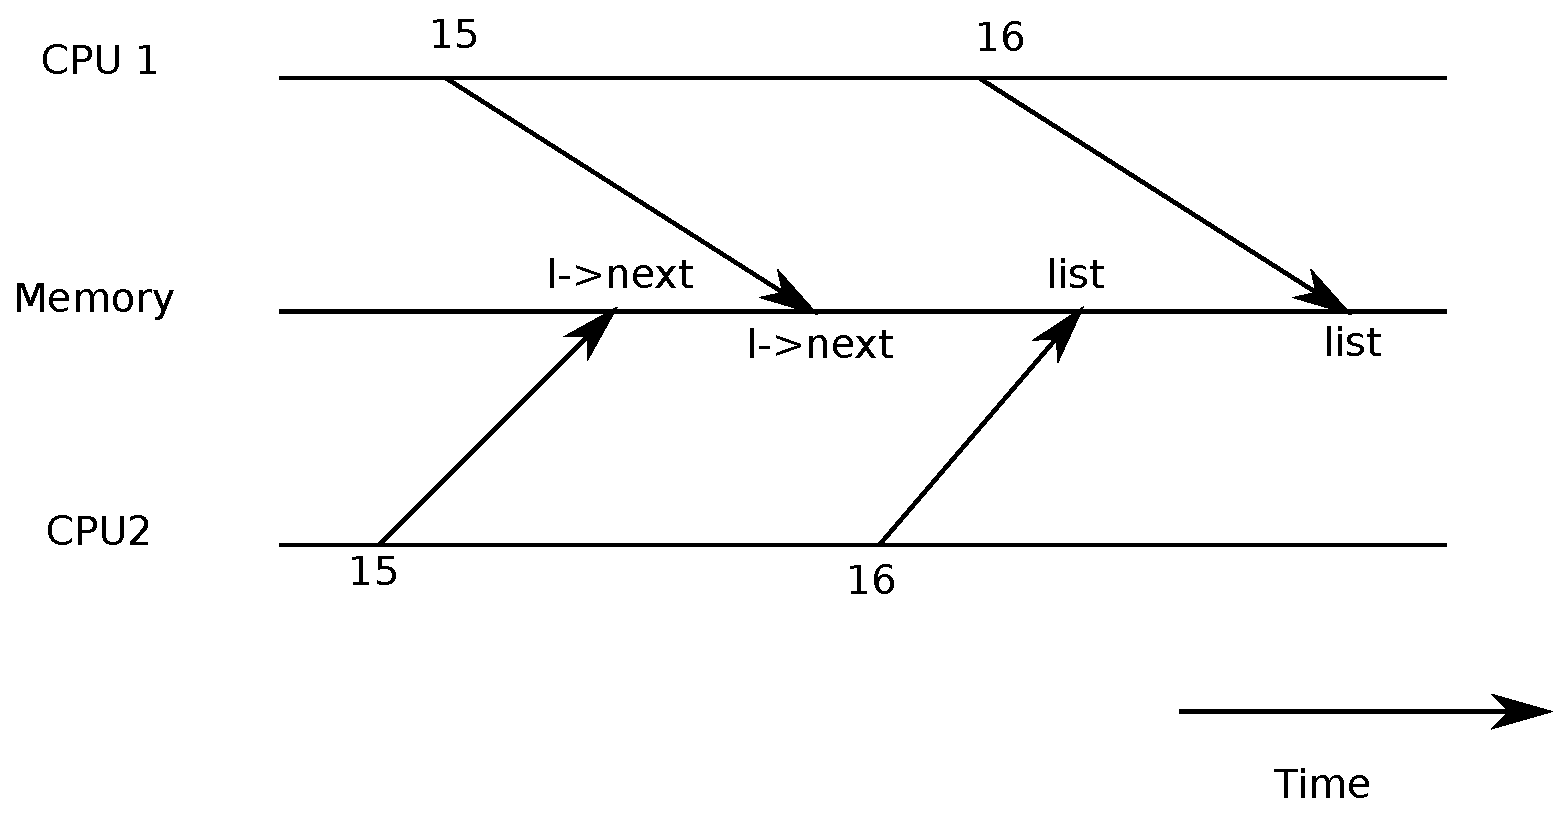
\includegraphics[scale=0.5]{fig/race.eps}
\caption{Example race}
\label{fig:race}
\end{figure}
This implementation is correct if executed in isolation.
However, the code is not correct if more than one
copy executes concurrently.
If two CPUs execute
\lstinline{push}
at the same time,
both might execute line 15
before either executes 16 (see 
Figure~\ref{fig:race}).
There would then be two
list elements with
\lstinline{next}
set to the former value of
\lstinline{list}.
When the two assignments to
\lstinline{list}
happen at line 16,
the second one will overwrite the first;
the element involved in the first assignment
will be lost.

The lost update at line 16 is an example of a
\textit{race condition}\index{race condition}.
A race condition is a situation in which a memory location is accessed
concurrently, and at least one access is a write.
A race is often a sign of a bug, either a lost update
(if the accesses are writes) or a read of
an incompletely-updated data structure.
The outcome of a race depends on
the exact timing of the two CPUs involved and
how their memory operations are ordered by the memory system,
which can make race-induced errors difficult to reproduce
and debug.
For example, adding print statements while debugging
\lstinline{push}
might change the timing of the execution enough
to make the race disappear.

The usual way to avoid races is to use a lock.
Locks ensure
\textit{mutual exclusion}\index{mutual exclusion},
so that only one CPU at a time can execute 
the sensitive lines of
\lstinline{push};
this makes the scenario above impossible.
The correctly locked version of the above code
adds just a few lines (not numbered):
\begin{lstlisting}[]
    6	struct element *list = 0;
     	struct lock listlock;
    7	
    8	void
    9	push(int data)
   10	{
   11	  struct element *l;
   12	  l = malloc(sizeof *l);
   13	  l->data = data;
   14	
     	  acquire(&listlock);
   15	  l->next = list;
   16	  list = l;
     	  release(&listlock);
   17	}
\end{lstlisting}
The sequence of instructions between
\lstinline{acquire}
and
\lstinline{release}
is often called a
\textit{critical section}\index{critical section},
and the lock protects
\lstinline{list}.

When we say that a lock protects data, we really mean
that the lock protects some collection of invariants
that apply to the data.
Invariants are properties of data structures that
are maintained across operations.
Typically, an operation's correct behavior depends
on the invariants being true when the operation
begins.  The operation may temporarily violate
the invariants but must reestablish them before
finishing.
For example, in the linked list case, the invariant is that
\lstinline{list}
points at the first element in the list
and that each element's
\lstinline{next}
field points at the next element.
The implementation of
\lstinline{push}
violates this invariant temporarily: in line 15,
\lstinline{l}
points
to the next list element, but
\lstinline{list}
does not point at
\lstinline{l}
yet (reestablished at line 16).
The race condition we examined above
happened because a second CPU executed
code that depended on the list invariants
while they were (temporarily) violated.
Proper use of a lock ensures that only one CPU at a time
can operate on the data structure in the critical section, so that
no CPU will execute a data structure operation when the 
data structure's invariants do not hold.

You can think of a lock as
\textit{serializing}\index{serializing}
concurrent critical sections so that they run one at a time,
and thus preserve invariants (assuming the critical sections
are correct in isolation).
You can also think of critical sections guarded by the same lock as being
atomic with respect to each other,
so that each sees only the complete set of
changes from earlier critical sections, and never sees
partially-completed updates.

Note that it would be correct to move
\lstinline{acquire}
earlier in
\lstinline{push.}
For example, it is fine to move the call to
\lstinline{acquire}
up to before line 12.
This may reduce parallelism because then the calls
to
\lstinline{malloc}
are also serialized.
The section "Using locks" below provides some guidelines for where to insert
\lstinline{acquire}
and
\lstinline{release}
invocations.
%% 
\section{Code: Locks}
%% 
Xv6 has two types of locks: spin-locks and sleep-locks.
We'll start with spin-locks.
Xv6 represents a spin-lock as a
\lstinline{struct spinlock}\index{struct spinlock@\lstinline{struct spinlock}}
\lineref{kernel/spinlock.h:/struct.spinlock/}.
The important field in the structure is
\lstinline{locked},
a word that is zero when the lock is available
and non-zero when it is held.
Logically, xv6 should acquire a lock by executing code like
\begin{lstlisting}[]
   21	void
   22	acquire(struct spinlock *lk)
   23	{
   24	  for(;;) {
   25	    if(lk->locked == 0) {
   26	      lk->locked = 1;
   27	      break;
   28	    }
   29	  }
   30	}
\end{lstlisting}
Unfortunately, this implementation does not
guarantee mutual exclusion on a multiprocessor.
It could happen that two CPUs simultaneously
reach line 25, see that 
\lstinline{lk->locked}
is zero, and then both grab the lock by executing line 26.
At this point, two different CPUs hold the lock,
which violates the mutual exclusion property.
What we need is a way to
make lines 25 and 26 execute as an
\textit{atomic}\index{atomic}
(i.e., indivisible) step.

Because locks are widely used,
multi-core processors usually provide instructions that
can be used to implement an atomic version of
lines 25 and 26.
On the RISC-V this instruction is
\lstinline{amoswap register, address}.
\lstinline{amoswap}
reads the value at the memory address,
writes the contents of the register to that address,
and puts the value it read into the register.
That is, it swaps the contents of the register and the memory address.
It performs this sequence atomically, using special
hardware to prevent any
other CPU from using the memory address between the read and the write.

Xv6's 
\lstinline{acquire}\index{acquire@\lstinline{acquire}}
\lineref{kernel/spinlock.c:/^acquire/}
uses the portable C library call 
\lstinline{__sync_lock_test_and_set},
which boils down to the
\lstinline{amoswap}
instruction;
the return value is the old (swapped) contents of
\lstinline{lk->locked}.
The
\lstinline{acquire}
function wraps the swap in a loop, retrying (spinning) until it has
acquired the lock.
Each iteration swaps one into
\lstinline{lk->locked} 
and checks the previous value;
if the previous value is zero, then we've acquired the
lock, and the swap will have set 
\lstinline{lk->locked}
to one.
If the previous value is one, then some other CPU
holds the lock, and the fact that we swapped one into
\lstinline{lk->locked}
didn't change its value.

Once the lock is acquired,
\lstinline{acquire}
records, for debugging, the CPU 
that acquired the lock.
The
\lstinline{lk->cpu}
field is protected by the lock
and must only be changed while holding the lock.

The function
\lstinline{release}\index{release@\lstinline{release}}
\lineref{kernel/spinlock.c:/^release/}
is the opposite of 
\lstinline{acquire}:
it clears the 
\lstinline{lk->cpu}
field
and then releases the lock.
Conceptually, the release just requires assigning zero to
\lstinline{lk->locked}.
The C standard allows compilers to implement assignment
with multiple store instructions,
so a C assignment might be non-atomic with respect
to concurrent code.
Instead,
\lstinline{release}
uses the C library function
\lstinline{__sync_lock_release}
that performs an atomic assignment.
This function also boils down to a RISC-V
\lstinline{amoswap}
instruction.
%% 
\section{Code: Using locks}
%% 
Xv6 uses locks in many places to avoid race conditions.
To see a simple example much like
\lstinline{push}
above,
look at
\lstinline{kalloc}
\lineref{kernel/kalloc.c:/^kalloc/}
and
\lstinline{free}
\lineref{kernel/kalloc.c:/^free/}.
Try Exercises 1 and 2 to see what happens if those
functions omit the locks.
You'll likely find that it's difficult to trigger incorrect
behavior, suggesting that it's hard to ensure that code
is free from locking errors and races.
It is not unlikely that xv6 has some races.

A hard part about using locks is deciding how many locks
to use and which data and invariants each lock should protect.
There are a few basic principles.
First, any time a variable can be written by one CPU
at the same time that another CPU can read or write it,
a lock should be introduced to keep the two
operations from overlapping.
Second, remember that locks protect invariants:
if an invariant involves multiple memory locations,
typically all of them need to be protected
by a single lock to ensure the invariant is maintained.

The rules above say when locks are necessary but say nothing about when locks
are unnecessary, and it is important for efficiency not to lock too much,
because locks reduce parallelism.  If parallelism isn't important, then one
could arrange to have only a single thread and not worry about locks.  A simple
kernel can do this on a multiprocessor by having a single lock that must be
acquired on entering the kernel and released on exiting the kernel (though
system calls such as pipe reads or
\lstinline{wait}
would pose a problem).  Many uniprocessor operating systems have been converted to
run on multiprocessors using this approach, sometimes called a ``giant
kernel lock,'' but the approach sacrifices parallelism: only one
CPU can execute in the kernel at a time.  If the kernel does any heavy
computation, it would be more efficient to use a larger set of more
fine-grained locks, so that the kernel could execute on multiple CPUs
simultaneously.

As an example of relatively coarse-grained locking, xv6's
\lstinline{kalloc.c}
allocator has a single free list protected by a single
lock. If concurrent allocation were a performance bottleneck,
it might be helpful to have multiple free lists, each with
its own lock, to allow truly parallel allocation.
As an example of relatively fine-grained locking, xv6
has a separate lock for each file, so that processes that
manipulate different files can often proceed without waiting
for each others' locks. On the other hand, this locking
scheme could be made even more fine-grained, if one wanted
to have good performance for processes that simultaneously
write different areas of the same file.
Ultimately lock granularity decisions need to be driven
by performance measurements as well as complexity considerations.

As subsequent chapters explain each part of xv6, they
will mention examples of xv6's use of locks
to deal with concurrency.
As a preview,
Figure~\ref{fig:locktable}
lists all of the locks in xv6.

\begin{figure}[t]
\center
\begin{tabular}{ll}
{\bf Lock} & {\bf Description} \\
\midrule
bcache.lock & Protects allocation of block buffer cache entries \\
cons.lock & Serializes access to console hardware, avoids intermixed output \\
ftable.lock & Serializes allocation of a struct file in file table \\
icache.lock & Protects allocation of inode cache entries \\
vdisk\_lock & Serializes access to disk hardware and queue of DMA descriptors \\
kmem.lock & Serializes allocation of memory \\
log.lock & Serializes operations on the transaction log \\
pipe's p->lock & Serializes operations on each pipe \\
pid\_lock & Serializes increments of next\_pid \\
proc's p->lock & Serializes changes to process's state \\
tickslock & Serializes operations on the ticks counter \\
inode's ip->lock & Serializes operations on each inode and its content \\
buf's b->lock & Serializes operations on each block buffer \\
\end{tabular}
\caption{Locks in xv6}
\label{fig:locktable}
\end{figure}
%% 
\section{Deadlock and lock ordering}
%% 
If a code path through the kernel must hold several locks at the same time, it is
important that all code paths acquire those locks in the same order.  If
they don't, there is a risk of deadlock.  Let's say two code paths in
xv6 need locks A and B, but code path 1 acquires locks in the order A
then B, and the other path acquires them in the order B then A.
Suppose thread T1 executes code path 1 and acquires lock A,
and thread T2 executes code path 2 and acquires lock B.
Next T1 will try to acquire lock B, and T2 will try to acquire lock A.
Both acquires will block indefinitely, because in both cases the
other thread holds the needed lock, and won't release it until
its acquire returns.
To avoid such deadlocks, all code paths must acquire
locks in the same order. The need for a global lock acquisition order
means that locks are effectively part of each function's specification: 
callers must invoke functions in a way that causes locks to be acquired
in the agreed-on order.

Xv6 has many lock-order chains of length two involving
per-process locks
(the lock in each
\lstinline{struct proc})
due to the way that
\lstinline{sleep}
works (see Chapter
\*[CH:SCHED]).
For example,
\lstinline{consoleintr}
\lineref{kernel/console.c:/^consoleintr/}
is the interrupt routine which handles typed characters.
When a newline arrives, any process that is waiting for
console input should be woken up.
To do this,
\lstinline{consoleintr}
holds
\lstinline{cons.lock}
while calling 
\lstinline{wakeup}\index{wakeup@\lstinline{wakeup}},
which acquires 
the waiting process's lock in order to wake it up.
In consequence, the global deadlock-avoiding
lock order includes the rule that
\lstinline{cons.lock}
must be acquired before any process lock.
The file system code contains xv6's longest lock chains.
For example, creating a file requires simultaneously
holding a lock on the directory, a lock on the new file's inode,
a lock on a disk block buffer, 
\lstinline{idelock},
and
\lstinline{ptable.lock}.
To avoid deadlock, file system code always acquires locks in the order 
mentioned in the previous sentence.
\section{Locks and interrupt handlers}
%% 
Some xv6 spin-locks protect data that is used by
both threads and interrupt handlers.
For example, the
\lstinline{clockintr}
timer interrupt handler might increment
\lstinline{ticks}\index{ticks@\lstinline{ticks}} 
\lineref{kernel/trap.c:/^clockintr/}
at about the same time that a kernel
thread reads
\lstinline{ticks} 
in
\lstinline{sys_sleep}\index{sys_sleep@\lstinline{sys_sleep}}
\lineref{kernel/sysproc.c:/ticks0.=.ticks/}.
The lock
\lstinline{tickslock}\index{tickslock@\lstinline{tickslock}}
serializes the two accesses.

The interaction of spin-locks and interrupts raises a potential danger.
Suppose
\lstinline{sys_sleep}\index{sys_sleep@\lstinline{sys_sleep}}
holds
\lstinline{tickslock}\index{tickslock@\lstinline{tickslock}},
and its CPU is interrupted by a timer interrupt.
\lstinline{clockintr}
would try to acquire
\lstinline{tickslock},
see it was held, and wait for it to be released.
In this situation,
\lstinline{tickslock}
will never be released: only
\lstinline{sys_sleep}
can release it, but
\lstinline{sys_sleep}
will not continue running until
\lstinline{clockintr}
returns.
So the processor will deadlock, and any code
that needs either lock will also freeze.

To avoid this situation, if a spin-lock is used by an interrupt handler,
a processor must never hold that lock with interrupts enabled.
Xv6 is more conservative: when a processor acquires any
lock, xv6 always disables interrupts on that processor.
Interrupts may still occur on other processors, so 
an interrupt's
\lstinline{acquire}
can wait for a thread to release a spin-lock; just not on the same processor.

xv6 re-enables interrupts when a processor holds no spin-locks; it must
do a little book-keeping to cope with nested critical sections.
\lstinline{acquire}
calls
\lstinline{push_off}\index{push_off@\lstinline{push_off}}
\lineref{kernel/spinlock.c:/^push_off/}
and
\lstinline{release}
calls
\lstinline{pop_off}\index{pop_off@\lstinline{pop_off}}
\lineref{kernel/spinlock.c:/^pop_off/}
to track the nesting level of locks on the current processor.
When that count reaches zero,
\lstinline{pop_off} 
restores the interrupt enable state that existed 
at the start of the outermost critical section.
The
\lstinline{intr_off}
and
\lstinline{intr_on}
functions execute RISC-V instructions to disable and enable
interrupts, respectively.

It is important that
\lstinline{acquire}\index{acquire@\lstinline{acquire}}
call
\lstinline{push_off}
strictly before setting
\lstinline{lk->locked}
\lineref{kernel/spinlock.c:/sync_lock_test_and_set/}.
If the two were reversed, there would be
a brief window when the lock
was held with interrupts enabled, and
an unfortunately timed interrupt would deadlock the system.
Similarly, it is important that
\lstinline{release}\index{release@\lstinline{release}}
call
\lstinline{pop_off}\index{pop_off@\lstinline{pop_off}}
only after 
releasing the lock
\lineref{kernel/spinlock.c:/sync_lock_release/}.
%% 
\section{Instruction and memory ordering}
%% 

It is natural to think of programs executing in the order
in which source code statements appear.
Many
compilers and processors, however, execute code out of order
to achieve
higher performance.  If an instruction takes many cycles to complete,
a processor may issue the instruction early so that it can
overlap with other instructions and avoid processor stalls. For
example, a processor may notice that in a serial sequence of
instructions A and B are not dependent on each other.
The processor may start instruction B first, either because its
inputs are ready before A's inputs, or in order to overlap
execution of A and B.
A compiler may perform a similar re-ordering by emitting instructions
for one statement before the instructions for a statement that precedes it
in the source.

Compilers and processors follow rules when they re-order to
ensure that they don't change the results of correctly-written
serial code.
However, the rules do allow re-ordering that
changes the results of concurrent code,
and can easily lead to incorrect behavior on multiprocessors.

For example, in this code for
\lstinline{push},
it would be a disaster if the compiler or processor moved the
store corresponding to
line 4 to a point after the
\lstinline{release}
on line 6:
\begin{lstlisting}[]
    1	  l = malloc(sizeof *l);
    2	  l->data = data;
    3	  acquire(&listlock);
    4	  l->next = list;
    5	  list = l;
    6	  release(&listlock);
\end{lstlisting}
If such a re-ordering occurred, there would be a window during
which another processor could acquire the lock,
observe the updated
\lstinline{list},
but see an uninitialized
\lstinline{list->next}.

To tell the hardware and compiler not to perform such re-orderings,
xv6 uses
\lstinline{__sync_synchronize()} 
in both
\lstinline{acquire}
and
\lstinline{release}.
\lstinline{__sync_synchronize()}
is a memory barrier:
it tells the compiler and CPU to not reorder loads or stores across the
barrier.
Xv6 worries about ordering only in
\lstinline{acquire}
and
\lstinline{release},
because it uses locks to guard all accesses to shared data (other than locks
themselves).
%% 
\section{Sleep locks}
%% 

Sometimes xv6 code needs to hold a lock for a long time. For example,
the file system (Chapter~\ref{CH:FS}) keeps a file locked while reading
and writing its content on the disk, and these disk operations can
take tens of milliseconds. Efficiency demands that the processor be
yielded while waiting so that other threads can make
progress, and this in turn means that xv6 needs locks that 
work well when held across context switches.
Xv6 provides such locks in the form of
\textit{sleep-locks}\index{sleep-locks}.

Xv6 sleep-locks support yielding the processor during their critical
sections. This property poses a design challenge: if thread T1 holds
lock L1 and has yielded the processor, and thread T2 wishes to acquire
L1, we have to ensure that T1 can execute while T2 is waiting so
that T1 can release L1. T2 can't use the spin-lock acquire
function here: it
spins with interrupts turned off, and that would prevent T1
from running. To avoid this deadlock, the sleep-lock acquire
routine
(called
\lstinline{acquiresleep})
yields the processor while waiting, and does not disable
interrupts.

\lstinline{acquiresleep}
\lineref{kernel/sleeplock.c:/^acquiresleep/}
uses techniques that will be explained in
Chapter~\ref{CH:SCHED}.
At a high level, a sleep-lock has a
\lstinline{locked}
field that is protected by a spinlock, and 
\lstinline{acquiresleep} 's
call to
\lstinline{sleep}
atomically yields the CPU and releases the spin-lock.
The result is that other threads can execute while
\lstinline{acquiresleep}
waits.

Because sleep-locks leave interrupts enabled, they cannot be
used in interrupt handlers.
Because
\lstinline{acquiresleep}
may yield the processor,
sleep-locks cannot be used inside spin-lock critical
sections (though spin-locks can be used inside sleep-lock
critical sections).

Spin-locks have low overhead, but they waste CPU time if they
are held for long periods when other CPUs are waiting
for them.
Thus they are best suited to short critical sections.
Xv6 uses sleep-locks in the file system,
where it is convenient to
be able to hold locks across lengthy disk operations.
%% 
\section{Real world}
%% 
Programming with locks remains challenging despite years of research
into concurrency primitives and parallelism.
It is often best to conceal locks within 
higher-level constructs like synchronized queues, although xv6 does not
do this.  If you program with locks, it is wise to use a tool that attempts to
identify race conditions, because it is easy to miss an invariant that requires
a lock.

Most operating systems support POSIX threads (Pthreads), which allow a user
process to have several threads running concurrently on different processors.
Pthreads has support for user-level locks, barriers, etc.  Supporting Pthreads requires
support from the operating system. For example, it should be the case that if
one pthread blocks in a system call, another pthread of the same process should
be able to run on that processor.  As another example, if a pthread changes its
process's address space (e.g., maps or unmaps memory), the kernel must arrange that
other processors that run threads of the same process update their hardware page
tables to reflect the change in the address space.  On the x86, this involves
shooting down the
\textit{Translation Look-aside Buffer (TLB)}\index{Translation Look-aside Buffer (TLB)}
of other processors using inter-processor interrupts (IPIs).

It is possible to implement locks without atomic instructions, but it is
expensive, and most operating systems use atomic instructions.

Locks can be expensive if many processors try to acquire the same lock
at the same time.  If one processor has a lock
cached in its local cache, and another processor must acquire the lock, then the
atomic instruction to update the cache line that holds the lock must move the line
from the one processor's cache to the other processor's cache, and perhaps
invalidate any other copies of the cache line.  Fetching a cache line from
another processor's cache can be orders of magnitude more expensive than
fetching a line from a local cache.

To avoid the expenses associated with locks, many operating systems use
lock-free data structures and algorithms.  For example, it is possible to
implement a linked list like the one in the beginning of the chapter that
requires no locks during list searches, and one atomic instruction to insert an
item in a list.  Lock-free programming is more complicated, however, than
programming locks; for example, one must worry about instruction and memory
reordering.  Programming with locks is already hard, so xv6 avoids the
additional complexity of lock-free programming.
%% 
\section{Exercises}
%% 

1. Comment out the calls to
\lstinline{acquire}
and
\lstinline{release}
in
\lstinline{kalloc}
\lineref{kernel/kalloc.c:/^kalloc/}.
This seems like it should cause problems for
kernel code that calls
\lstinline{kalloc};
what symptoms do you expect to see?
When you run xv6, do you see these symptoms?
How about when running
\lstinline{usertests} ?
If you don't see a problem, why not?
See if you can provoke a problem by inserting
dummy loops into the critical section of
\lstinline{kalloc}.

2. Suppose that you instead commented out the
locking in
\lstinline{kfree} 
(after restoring locking in
\lstinline{kalloc}).
What might now go wrong? Is lack of locks in
\lstinline{kfree}
less harmful than in
\lstinline{kalloc} ?

3. If two CPUs call
\lstinline{kalloc}
at the same time, one will have to wait for the other,
which is bad for performance.
Modify 
\lstinline{kalloc.c}
to have more parallelism, so that simultaneous
calls to
\lstinline{kalloc}
from different CPUs can proceed without waiting for each other.

4. Write a parallel program using POSIX threads, which is supported on most
operating systems. For example, implement a parallel hash table and measure if
the number of puts/gets scales with increasing number of cores.

5. Implement a subset of Pthreads in xv6.  That is, implement a user-level
thread library so that a user process can have more than 1 thread and arrange
that these threads can run in parallel on different processors.  Come up with a
design that correctly handles a thread making a blocking system call and
changing its shared address space.

% cox and mullender, semaphores.
% 
% process has one thread with two stacks
%  
% pike et al, sleep and wakeup
\chapter{Scheduling}
\label{CH:SCHED}

Any operating system is likely to run with more processes than the
computer has processors, so a plan is needed to time-share the
processors among the processes. Ideally the sharing would be transparent to user
processes.  A common approach is to provide each process
with the illusion that it has its own virtual processor by
\textit{multiplexing}\index{multiplexing}
the processes onto the hardware processors.
This chapter explains how xv6 achieves this multiplexing.
%% 
\section{Multiplexing}
%% 

Xv6 multiplexes by switching each processor from one process to
another in two situations. First, xv6's
\lstinline{sleep}
and
\lstinline{wakeup}
mechanism switches when a process waits
for device or pipe I/O to complete, or waits for a child
to exit, or waits in the
\lstinline{sleep}
system call.
Second, xv6 periodically forces a switch to cope with
processes that compute for long periods without sleeping.
This multiplexing creates the illusion that
each process has its own CPU, just as xv6 uses the memory allocator and hardware
page tables to create the illusion that each process has its own memory.

Implementing multiplexing poses a few challenges. First, how to switch from one
process to another? 
Although the idea of context switching
is simple, the implementation is some of the most opaque code
in xv6. Second, how to force
switches in a way that is transparent to user processes?  Xv6 uses the
standard technique of driving context switches with timer interrupts.
Third, many CPUs may be switching among processes concurrently, and a
locking plan is necessary to avoid races. Fourth, a process's
memory and other resources must be freed when the process exits,
but it cannot do all of this itself
because (for example) it can't free its own kernel stack while still using it.
Finally, each core of a multi-core machine must remember which
process it is executing so that system calls affect the correct
process's kernel state.
Xv6 tries to solve these problems as
simply as possible, but nevertheless the resulting code is
tricky.

xv6 must provide
ways for processes to coordinate among themselves. For example,
a parent process may need to wait for one of its children to
exit, or a process reading a pipe may need to wait for
some other process to write the pipe.
Rather than make the waiting process waste CPU by repeatedly checking
whether the desired event has happened, xv6 allows a process to give
up the CPU and sleep
waiting for an event, and allows another process to wake the first
process up. Care is needed to avoid races that result in
the loss of event notifications.
%% 
\section{Code: Context switching}
%% 

\begin{figure}[t]
\center
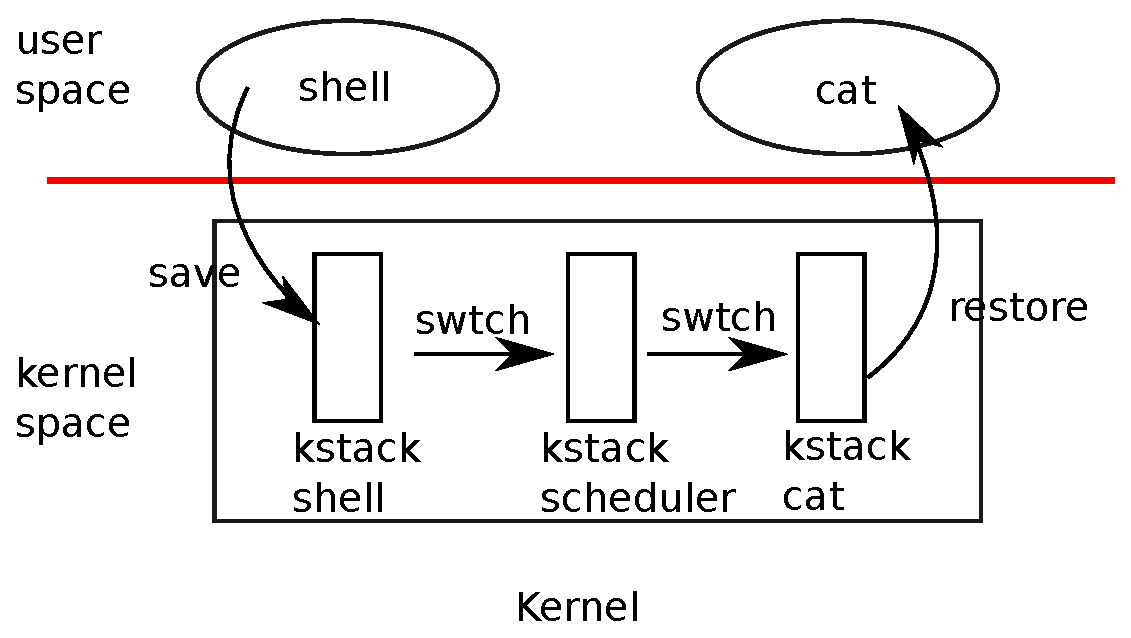
\includegraphics[scale=0.5]{fig/switch.eps}
\caption{Switching from one user process to another.  In this example, xv6 runs with one CPU (and thus one scheduler thread).}
\label{fig:switch}
\end{figure}

Figure~\ref{fig:switch} 
outlines the steps involved in switching from one
user process to another:
a user-kernel transition (system
call or interrupt) to the old process's kernel thread,
a context switch to the current CPU's scheduler thread, a context
switch to a new process's kernel thread, and a trap return
to the user-level process.
The xv6 scheduler has a dedicate thread (saved registers and stack)
per CPU because
it is sometimes not safe for it execute on
any process's kernel stack;
we'll see an example in
\lstinline{exit}.
In this section we'll examine the mechanics of switching
between a kernel thread and a scheduler thread.

Switching from one thread to another involves saving the old thread's
CPU registers, and restoring the previously-saved registers of the
new thread; the fact that
the stack pointer and program counter
are saved and restored means that the CPU will switch stacks and
switch what code it is executing.

The function
\indexcode{swtch}
performs the saves and restores for a thread switch.
\lstinline{swtch}
doesn't directly know about threads; it just saves and
restores register sets, called 
\textit{contexts}\index{contexts}.
When it is time for a process to give up the CPU,
the process's kernel thread calls
\lstinline{swtch}
to save its own context and return to the scheduler context.
Each context is represented by a
\lstinline{struct}
\lstinline{context*}
\lineref{kernel/proc.h:/^struct.context/},
a pointer to a structure stored on the kernel stack involved.
\lstinline{Swtch}
takes two arguments:
\indexcode{struct context}
\lstinline{**old}
and
\lstinline{struct}
\lstinline{context}
\lstinline{*new}.
It pushes the current registers onto the stack
and saves the stack pointer in
\lstinline{*old}.
Then
\lstinline{swtch}
copies
\lstinline{new}
to 
\texttt{\%rsp},
pops previously saved registers, and returns.

Let's follow a user process through
\lstinline{swtch} 
into the scheduler.
We saw in Chapter~\ref{CH:TRAP}
that one possibility at the end of each interrupt
is that 
\indexcode{trap}
calls 
\indexcode{yield}.
\lstinline{Yield}
in turn calls
\indexcode{sched},
which calls
\indexcode{swtch}
to save the current context in
\lstinline{proc->context}
and switch to the scheduler context previously saved in 
\indexcode{cpu->scheduler}
\lineref{kernel/proc.c:/swtch..p/}.

\lstinline{Swtch}
\lineref{kernel/swtch.S:/swtch/}
pushes the register state, creating a context structure
on the current stack.
Only the callee-saved registers need to be saved;
the convention on the x86-64 is that these are
\texttt{\%rbp},
\texttt{\%rbx},
\texttt{\%r11}
through
\texttt{\%r15},
and
\texttt{\%rsp}.
\lstinline{Swtch}
pushes the first 7 explicitly
\linerefs{kernel/swtch.S:/push..rbp/,/push..r15/};
it saves the last implicitly as the
\lstinline{struct}
\lstinline{context*}
written to
\lstinline{*old} 
\lineref{kernel/swtch.S:/mov..rsp/}.
There is one more important register:
the program counter 
\texttt{\%eip}.
It has already been saved on the stack by the
\lstinline{call}
instruction that invoked
\lstinline{swtch}.
Having saved the old context,
\lstinline{swtch}
is ready to restore the new one.
It moves the pointer to the new context
into the stack pointer
\lineref{kernel/swtch.S:/mov..rsi/}.
The new stack has the same form as the old one that
\indexcode{swtch}
just left—the new stack
\textit{was}
the old one in a previous call to
\lstinline{swtch} —\c
so 
\lstinline{swtch}
can invert the sequence to restore the new context.
It pops the values for
\texttt{\%r15}
through
\texttt{\%r11},
and
\texttt{\%rbx},
and
\texttt{\%rbp},
and then returns
\linerefs{kernel/swtch.S:/pop/,/ret/}.
Because 
\lstinline{swtch}
has changed the stack pointer, the values restored
and the instruction address returned to
are the ones from the new context.

In our example, 
\indexcode{sched}
called
\indexcode{swtch}
to switch to
\indexcode{cpu->scheduler},
the per-CPU scheduler context.
That context had been saved by 
\lstinline{scheduler} 's
call to
\lstinline{swtch}
\lineref{kernel/proc.c:/swtch.&.c/}.
When the
\indexcode{swtch}
we have been tracing returns,
it returns not to
\lstinline{sched}
but to 
\indexcode{scheduler},
and its stack pointer points at the current CPU's
scheduler stack.
%% 
\section{Code: Scheduling}
%% 

The last section looked at the low-level details of
\indexcode{swtch};
now let's take 
\lstinline{swtch}
as a given and examine 
switching from a process through the scheduler to another process.
A process
that wants to give up the CPU must
acquire the process table lock
\indexcode{ptable.lock},
release any other locks it is holding,
update its own state
(\lstinline{proc->state}),
and then call
\indexcode{sched}.
\lstinline{Yield}
\lineref{kernel/proc.c:/^yield/}
follows this convention, as do
\indexcode{sleep}
and
\indexcode{exit},
which we will examine later.
\lstinline{Sched}
double-checks those conditions
\linerefs{kernel/proc.c:/if..holding/,/running/}
and then an implication of those conditions:
since a lock is held, the CPU should be
running with interrupts disabled.
Finally,
\indexcode{sched}
calls
\indexcode{swtch}
to save the current context in 
\lstinline{proc->context}
and switch to the scheduler context in
\indexcode{cpu->scheduler}.
\lstinline{Swtch}
returns on the scheduler's stack
as though
\indexcode{scheduler} 's
\lstinline{swtch}
had returned
\lineref{kernel/proc.c:/swtch.&.c/}.
The scheduler continues the 
\lstinline{for}
loop, finds a process to run, 
switches to it, and the cycle repeats.

We just saw that xv6 holds
\indexcode{ptable.lock}
across calls to
\lstinline{swtch}:
the caller of
\indexcode{swtch}
must already hold the lock, and control of the lock passes to the
switched-to code.  This convention is unusual with locks; usually
the thread that acquires a lock is also responsible for
releasing the lock, which makes it easier to reason about correctness.
For context switching it is necessary to break this convention because
\indexcode{ptable.lock}
protects invariants on the process's
\lstinline{state}
and
\lstinline{context}
fields that are not true while executing in
\lstinline{swtch}.
One example of a problem that could arise if
\lstinline{ptable.lock}
were not held during
\indexcode{swtch}:
a different CPU might decide
to run the process after 
\indexcode{yield}
had set its state to
\lstinline{RUNNABLE},
but before 
\lstinline{swtch}
caused it to stop using its own kernel stack.
The result would be two CPUs running on the same stack,
which cannot be right.

A kernel thread always gives up its
processor in
\lstinline{sched} 
and always switches to the same location in the scheduler, which
(almost) always switches to some kernel thread that previously called
\lstinline{sched}. 
Thus, if one were to print out the line numbers where xv6 switches
threads, one would observe the following simple pattern:
\lineref{kernel/proc.c:/swtch.&.c/},
\lineref{kernel/proc.c:/swtch..p/},
\lineref{kernel/proc.c:/swtch.&.c/},
\lineref{kernel/proc.c:/swtch..p/},
and so on.  The procedures in which this stylized switching between
two threads happens are sometimes referred to as 
\textit{coroutines}\index{coroutines}; 
in this example,
\indexcode{sched}
and
\indexcode{scheduler}
are co-routines of each other.

There is one case when the scheduler's call to
\indexcode{swtch}
does not end up in
\indexcode{sched}.
We saw this case in Chapter~\ref{CH:MEM}: when a
new process is first scheduled, it begins at
\indexcode{forkret}
\lineref{kernel/proc.c:/^forkret/}.
\lstinline{Forkret}
exists to release the 
\indexcode{ptable.lock};
otherwise, the new process could start at
\lstinline{trapret}.

\lstinline{Scheduler}
\lineref{kernel/proc.c:/^scheduler/} 
runs a simple loop:
find a process to run, run it until it yields, repeat.
\indexcode{scheduler}
holds
\indexcode{ptable.lock}
for most of its actions,
but releases the lock (and explicitly enables interrupts)
once in each iteration of its outer loop.
This is important for the special case in which this CPU
is idle (can find no
\lstinline{RUNNABLE}
process).
If an idling scheduler looped with
the lock continuously held, no other CPU that
was running a process could ever perform a context
switch or any process-related system call,
and in particular could never mark a process as
\indexcode{RUNNABLE}
so as to break the idling CPU out of its scheduling loop.
The reason to enable interrupts periodically on an idling
CPU is that there might be no
\lstinline{RUNNABLE}
process because processes (e.g., the shell) are
waiting for I/O;
if the scheduler left interrupts disabled all the time,
the I/O would never arrive.

The scheduler
loops over the process table
looking for a runnable process, one that has
\lstinline{p->state} 
\lstinline{==}
\lstinline{RUNNABLE}.
Once it finds a process, it sets the per-CPU current process
variable
\lstinline{proc},
switches to the process's page table with
\indexcode{switchuvm},
marks the process as
\lstinline{RUNNING},
and then calls
\indexcode{swtch}
to start running it
\linerefs{kernel/proc.c:/Switch.to/,/swtch/}.

One way to think about the structure of the scheduling code is
that it arranges to enforce a set of invariants about each process,
and holds
\indexcode{ptable.lock}
whenever those invariants are not true.
One invariant is that if a process is
\lstinline{RUNNING},
a timer interrupt's
\indexcode{yield}
must be able to switch away from the process;
this means that the CPU registers must hold the process's register values
(i.e. they aren't actually in a
\lstinline{context}),
\texttt{\%cr3}
must refer to the process's pagetable,
\texttt{\%esp}
must refer to the process's kernel stack so that
\lstinline{swtch}
can push registers correctly, and
\lstinline{proc}
must refer to the process's
\lstinline{proc[]}
slot.
Another invariant is that if a process is
\indexcode{RUNNABLE},
an idle CPU's
\indexcode{scheduler}
must be able to run it;
this means that 
\indexcode{p->context}
must hold the process's kernel thread variables,
that no CPU is executing on the process's kernel stack,
that no CPU's
\texttt{\%cr3}
refers to the process's page table,
and that no CPU's
\lstinline{proc}
refers to the process.

Maintaining the above invariants is the reason why xv6 acquires 
\indexcode{ptable.lock}
in one thread (often in
\lstinline{yield)}
and releases the lock in a different thread
(the scheduler thread or another next kernel thread).
Once the code has started to modify a running process's state
to make it
\lstinline{RUNNABLE},
it must hold the lock until it has finished restoring
the invariants: the earliest correct release point is after
\lstinline{scheduler}
stops using the process's page table and clears
\lstinline{proc}.
Similarly, once 
\lstinline{scheduler}
starts to convert a runnable process to
\lstinline{RUNNING},
the lock cannot be released until the kernel thread
is completely running (after the
\lstinline{swtch},
e.g. in
\lstinline{yield}).

\indexcode{ptable.lock}
protects other things as well:
allocation of process IDs and free process table slots,
the interplay between
\indexcode{exit}
and
\indexcode{wait},
the machinery to avoid lost wakeups (see next section),
and probably other things too.
It might be worth thinking about whether the 
different functions of
\lstinline{ptable.lock}
could be split up, certainly for clarity and perhaps
for performance.
%% 
\section{Code: mycpu and myproc}
%% 

As we saw in Chapter~\ref{CH:TRAP},
xv6 maintains a
\indexcode{struct cpu}
for each processor, which records
the process currently running
on the processor (if any),
the processor's unique hardware identifier
(\lstinline{apicid}),
and some other information.
The function
\indexcode{getmycpu}
\lineref{kernel/proc.c:/^getmycpu/}
returns the current processor's
\lstinline{struct cpu}.
\lstinline{getmycpu}
does this by reading the processor
identifier from the local APIC hardware and looking through
the array of
\lstinline{struct cpu}
for an entry with that identifier.
The function 
\lstinline{seginit}
\lineref{kernel/vm.c:/^seginit/}
programs the register
\lstinline{MSR_GS_KERNBASE}
to contain a pointer to the core's
\lstinline{struct cpu}.
The function
\indexcode{mycpu}
\lineref{kernel/proc.c:/^mycpu/}
returns that
value using
\texttt{\%gs}.
Using
\texttt{\%gs}
avoids every call to
\lstinline{mycpu}
having to loop
through the array
\lstinline{cpus},
as
\lstinline{getmycpu}
does.

The return value of
\lstinline{getmycpu}
and
\lstinline{mycpu}
are fragile: if the timer were to interrupt and cause
the thread to be moved to a different processor, the
return value would no longer be correct.
To avoid this problem, xv6 requires that callers of
\lstinline{getmycpu}
disable interrupts, and only enable
them after they finish using the returned
\lstinline{struct cpu}.

The function
\indexcode{myproc}
\lineref{kernel/proc.c:/^myproc/}
returns the
\lstinline{struct proc}
pointer
for the process that is running on the current processor.
\lstinline{myproc}
disables interrupts, invokes
\lstinline{mycpu},
fetches the current process pointer
(\lstinline{c->proc})
out of the
\lstinline{struct cpu},
and then enables interrupts.
If there is no process running, because the the caller is
executing in
\lstinline{scheduler},
\lstinline{myproc}
returns zero.
The return value of
\lstinline{myproc}
is safe to use even if interrupts are enabled:
if a timer interrupt moves the calling process to a
different processor, its
\lstinline{struct proc}
pointer will stay the same.
%% 
\section{Sleep and wakeup}
%% 

Scheduling and locks help conceal the existence of one process
from another,
but so far we have no abstractions that help
processes intentionally interact.
Sleep and wakeup fill that void, allowing one process to 
sleep waiting for an event and another process to wake it up
once the event has happened.
Sleep and wakeup are often called 
\textit{sequence coordination}\index{sequence coordination}
or 
\textit{conditional synchronization}\index{conditional synchronization}
mechanisms, and there are many other similar mechanisms
in the operating systems literature.

To illustrate what we mean, let's consider a
simple producer/consumer queue.
XXX This queue is similar to the one that feeds commands from processes
to the virtio driver
(see Chapter~\ref{CH:TRAP}), but abstracts away all
IDE-specific code.
The queue allows one process to send a nonzero pointer
to another process.
If there were only one sender and one receiver,
and they executed on different CPUs,
and the compiler didn't optimize too agressively,
this implementation would be correct:
\begin{lstlisting}[]
  100	struct q {
  101	  void *ptr;
  102	};
  103	
  104	void*
  105	send(struct q *q, void *p)
  106	{
  107	  while(q->ptr != 0)
  108	    ;
  109	  q->ptr = p;
  110	}
  111	
  112	void*
  113	recv(struct q *q)
  114	{
  115	  void *p;
  116	
  117	  while((p = q->ptr) == 0)
  118	    ;
  119	  q->ptr = 0;
  120	  return p;
  121	}
\end{lstlisting}
\lstinline{Send}
loops until the queue is empty
\lstinline{ptr} "" (
\lstinline{==}
\lstinline{0)}
and then puts the pointer
\lstinline{p}
in the queue.
\lstinline{Recv}
loops until the queue is non-empty
and takes the pointer out.
When run in different processes,
\lstinline{send}
and
\lstinline{recv}
both modify
\lstinline{q->ptr},
but
\lstinline{send}
only writes the pointer when it is zero
and
\lstinline{recv}
only writes the pointer when it is nonzero,
so no updates are lost.

The implementation above 
is expensive.  If the sender sends
rarely, the receiver will spend most
of its time spinning in the 
\lstinline{while}
loop hoping for a pointer.
The receiver's CPU could find more productive work than
\textit{busy waiting}\index{busy waiting}
by repeatedly 
\textit{polling}\index{polling}
\lstinline{q->ptr}.
Avoiding busy waiting requires
a way for the receiver to yield the CPU
and resume only when 
\lstinline{send}
delivers a pointer.

Let's imagine a pair of calls, 
\indexcode{sleep}
and
\indexcode{wakeup},
that work as follows.
\lstinline{Sleep(chan)}
sleeps on the arbitrary value
\indexcode{chan},
called the 
\textit{wait channel}\index{wait channel}.
\lstinline{Sleep}
puts the calling process to sleep, releasing the CPU
for other work.
\lstinline{Wakeup(chan)}
wakes all processes sleeping on
\lstinline{chan}
(if any), causing their
\lstinline{sleep}
calls to return.
If no processes are waiting on
\lstinline{chan},
\lstinline{wakeup}
does nothing.
We can change the queue implementation to use
\lstinline{sleep}
and
\lstinline{wakeup}:
\begin{lstlisting}[]
  201	void*
  202	send(struct q *q, void *p)
  203	{
  204	  while(q->ptr != 0)
  205	    ;
  206	  q->ptr = p;
  207	  wakeup(q);  /* wake recv */
  208	}
  209	
  210	void*
  211	recv(struct q *q)
  212	{
  213	  void *p;
  214	
  215	  while((p = q->ptr) == 0)
  216	    sleep(q);
  217	  q->ptr = 0;
  218	  return p;
  219	}
\end{lstlisting}

\begin{figure}[t]
\center
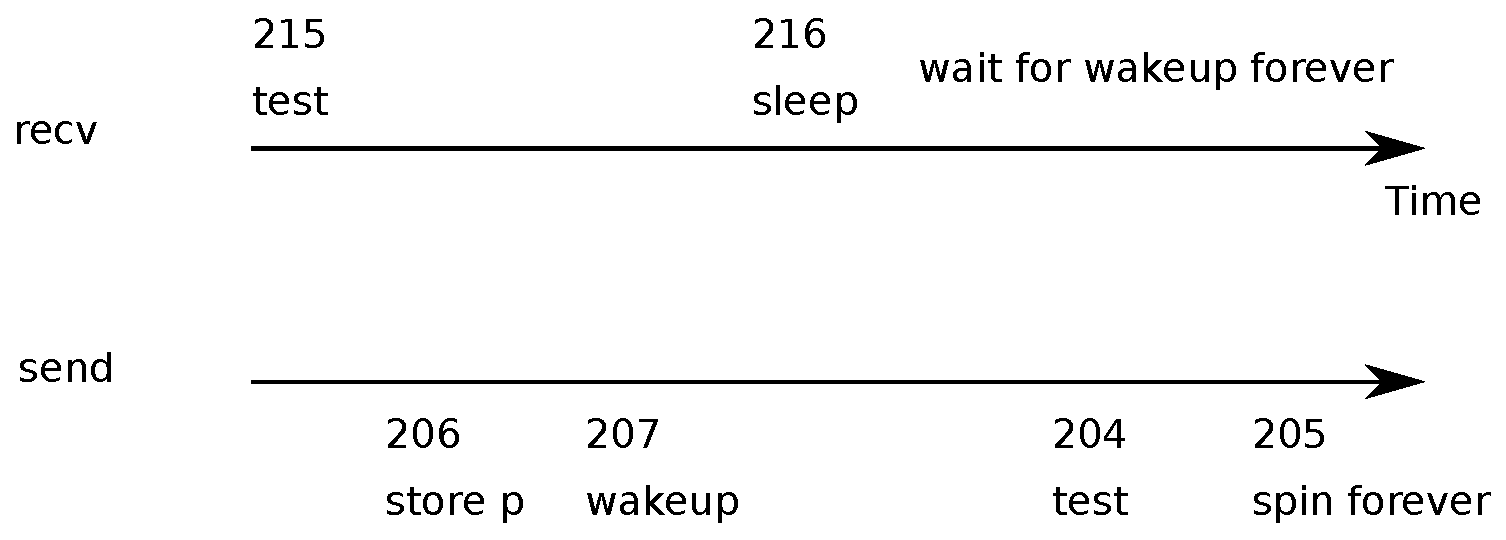
\includegraphics[scale=0.5]{fig/deadlock.eps}
\caption{Example lost wakeup problem}
\label{fig:deadlock}
\end{figure}

\lstinline{Recv}
now gives up the CPU instead of spinning, which is nice.
However, it turns out not to be straightforward to design
\lstinline{sleep}
and 
\lstinline{wakeup}
with this interface without suffering
from what is known as the ``lost wake-up'' problem (see 
Figure~\ref{fig:deadlock}).
Suppose that
\lstinline{recv}
finds that
\lstinline{q->ptr}
\lstinline{==}
\lstinline{0} 
on line 215.
While
\lstinline{recv}
is between lines 215 and 216,
\lstinline{send}
runs on another CPU:
it changes
\lstinline{q->ptr}
to be nonzero and calls
\lstinline{wakeup},
which finds no processes sleeping and thus does nothing.
Now
\lstinline{recv}
continues executing at line 216:
it calls
\lstinline{sleep}
and goes to sleep.
This causes a problem:
\lstinline{recv}
is asleep waiting for a pointer
that has already arrived.
The next
\lstinline{send}
will wait for 
\lstinline{recv}
to consume the pointer in the queue,
at which point the system will be 
\textit{deadlocked}\index{deadlocked}.

The root of this problem is that the
invariant that
\lstinline{recv}
only sleeps when
\lstinline{q->ptr}
\lstinline{==}
\lstinline{0}
is violated by 
\lstinline{send}
running at just the wrong moment.
One incorrect way of protecting the invariant would be to modify the code for
\lstinline{recv}
as follows:
\begin{lstlisting}[]
  300	struct q {
  301	  struct spinlock lock;
  302	  void *ptr;
  303	};
  304	
  305	void*
  306	send(struct q *q, void *p)
  307	{
  308	  acquire(&q->lock);
  309	  while(q->ptr != 0)
  310	    ;
  311	  q->ptr = p;
  312	  wakeup(q);
  313	  release(&q->lock);
  314	}
  315	
  316	void*
  317	recv(struct q *q)
  318	{
  319	  void *p;
  320	
  321	  acquire(&q->lock);
  322	  while((p = q->ptr) == 0)
  323	    sleep(q);
  324	  q->ptr = 0;
  325	  release(&q->lock);
  326	  return p;
  327	}
\end{lstlisting}
One might hope that this version of
\lstinline{recv}
would avoid the lost wakeup because the lock prevents
\lstinline{send}
from executing between lines 322 and 323.
It does that, but it also deadlocks:
\lstinline{recv}
holds the lock while it sleeps,
so the sender will block forever waiting for the lock.

We'll fix the preceding scheme by changing
\lstinline{sleep} 's
interface:
the caller must pass the lock to
\lstinline{sleep}
so it can release the lock after
the calling process is marked as asleep and waiting on the
sleep channel.
The lock will force a concurrent
\lstinline{send}
to wait until the receiver has finished putting itself to sleep,
so that the
\lstinline{wakeup}
will find the sleeping receiver and wake it up.
Once the receiver is awake again
\indexcode{sleep}
reacquires the lock before returning.
Our new correct scheme is useable as follows:
\begin{lstlisting}[]
  400	struct q {
  401	  struct spinlock lock;
  402	  void *ptr;
  403	};
  404	
  405	void*
  406	send(struct q *q, void *p)
  407	{
  408	  acquire(&q->lock);
  409	  while(q->ptr != 0)
  410	    ;
  411	  q->ptr = p;
  412	  wakeup(q);
  413	  release(&q->lock);
  414	}
  415	
  416	void*
  417	recv(struct q *q)
  418	{
  419	  void *p;
  420	
  421	  acquire(&q->lock);
  422	  while((p = q->ptr) == 0)
  423	    sleep(q, &q->lock);
  424	  q->ptr = 0;
  425	  release(&q->lock);
  426	  return p;
  427	}
\end{lstlisting}

The fact that
\lstinline{recv}
holds
\lstinline{q->lock}
prevents 
\lstinline{send}
from trying to wake it up between 
\lstinline{recv} 's
check of
\lstinline{q->ptr}
and its call to
\lstinline{sleep}.
We need
\lstinline{sleep}
to atomically release
\lstinline{q->lock}
and put the receiving process to sleep.

A complete sender/receiver implementation would also sleep
in
\lstinline{send}
when waiting for a receiver to consume
the value from a previous
\lstinline{send}.
%% 
\section{Code: Sleep and wakeup}
%% 

Let's look at the implementation of
\indexcode{sleep}
\lineref{kernel/proc.c:/^sleep/}
and
\indexcode{wakeup}
\lineref{kernel/proc.c:/^wakeup/}.
The basic idea is to have
\lstinline{sleep}
mark the current process as
\indexcode{SLEEPING}
and then call
\indexcode{sched}
to release the processor;
\lstinline{wakeup}
looks for a process sleeping on the given wait channel
and marks it as 
\indexcode{RUNNABLE}.
Callers of
\lstinline{sleep}
and
\lstinline{wakeup}
can use any mutually convenient number as the channel.
Xv6 often uses the address
of a kernel data structure involved in the waiting.

\lstinline{Sleep}
\lineref{kernel/proc.c:/^sleep/}
begins with a few sanity checks:
there must be a current process
\lineref{kernel/proc.c:/p.==.0/}
and
\lstinline{sleep}
must have been passed a lock
\linerefs{kernel/proc.c:/lk == 0/,/sleep.without/}.
Then 
\lstinline{sleep}
acquires 
\indexcode{ptable.lock}
\lineref{kernel/proc.c:/sleeplock1/}.
Now the process going to sleep holds both
\lstinline{ptable.lock}
and
\lstinline{lk}.
Holding
\lstinline{lk}
was necessary in the caller (in the example,
\lstinline{recv}):
it
ensured that no other process (in the example,
one running
\lstinline{send})
could start a call to
\lstinline{wakeup(chan)}.
Now that
\lstinline{sleep}
holds
\lstinline{ptable.lock},
it is safe to release
\lstinline{lk}:
some other process may start a call to
\lstinline{wakeup(chan)},
but
\indexcode{wakeup}
will not run until it can acquire
\indexcode{ptable.lock},
so it must wait until
\lstinline{sleep}
has finished putting the process to sleep,
keeping the
\lstinline{wakeup}
from missing the
\lstinline{sleep}.

There is a minor complication: if 
\lstinline{lk}
is equal to
\lstinline{&ptable.lock},
then
\lstinline{sleep}
would deadlock trying to acquire it as
\lstinline{&ptable.lock}
and then release it as
\lstinline{lk}.
In this case,
\lstinline{sleep}
considers the acquire and release
to cancel each other out
and skips them entirely
\lineref{kernel/proc.c:/sleeplock0/}.
For example,
\lstinline{wait}
\lineref{kernel/proc.c:/^wakeup\(/}
calls
\lstinline{sleep}
with 
\lstinline{&ptable.lock}.

Now that
\lstinline{sleep}
holds
\lstinline{ptable.lock}
and no others,
it can put the process to sleep by recording
the sleep channel,
changing the process state,
and calling
\lstinline{sched}
\lineref{kernel/proc.c:/chan.=.chan/,/sched/}.

At some point later, a process will call
\lstinline{wakeup(chan)}.
\lstinline{Wakeup}
\lineref{'kernel/proc.c:/^wakeup\(/}'
acquires
\indexcode{ptable.lock}
and calls
\indexcode{wakeup1},
which does the real work.
It is important that
\indexcode{wakeup}
hold the
\lstinline{ptable.lock}
both because it is manipulating process states
and because, as we just saw,
\lstinline{ptable.lock}
makes sure that
\lstinline{sleep}
and
\lstinline{wakeup}
do not miss each other.
\lstinline{Wakeup1}
is a separate function because
sometimes the scheduler needs to
execute a wakeup when it already
holds the 
\lstinline{ptable.lock};
we will see an example of this later.
\lstinline{Wakeup1}
\lineref{kernel/proc.c:/^wakeup1/}
loops over the process table.
When it finds a process in state
\indexcode{SLEEPING}
with a matching
\indexcode{chan},
it changes that process's state to
\indexcode{RUNNABLE}.
The next time the scheduler runs, it will
see that the process is ready to be run.

Xv6 code always calls
\lstinline{wakeup}
while holding the lock that guards the sleep condition;
in the example above that lock is
\lstinline{q->lock}.
Strictly speaking it is sufficient if
\lstinline{wakeup}
always follows the
\lstinline{acquire}
(that is, one could call
\lstinline{wakeup}
after the
\lstinline{release}).
Why do the locking rules for 
\lstinline{sleep}
and
\lstinline{wakeup}
ensure a sleeping process won't miss a wakeup it needs?
The sleeping process holds either
the lock on the condition or the
\lstinline{ptable.lock} 
or both from a point before it checks the condition
to a point after it is marked as sleeping.
If a concurrent thread causes the condition to be true,
that thread must either hold the lock on the condition before the
sleeping thread acquired it, or after the sleeping
thread released it in
\lstinline{sleep}.
If before, the sleeping thread must have seen the new condition
value, and decided to sleep anyway, so it doesn't matter
if it misses the wakeup.
If after, then the earliest the waker could acquire the
lock on the condition is after
\lstinline{sleep}
acquires
\lstinline{ptable.lock},
so that
\lstinline{wakeup} 's
acquisition of
\lstinline{ptable.lock}
must wait until
\lstinline{sleep}
has completely finished putting the sleeper to sleep.
Then 
\lstinline{wakeup}
will see the sleeping process and wake it up
(unless something else wakes it up first).

It is sometimes the case that multiple processes are sleeping
on the same channel; for example, more than one process
reading from a pipe.
A single call to 
\lstinline{wakeup}
will wake them all up.
One of them will run first and acquire the lock that
\lstinline{sleep}
was called with, and (in the case of pipes) read whatever
data is waiting in the pipe.
The other processes will find that, despite being woken up,
there is no data to be read.
From their point of view the wakeup was ``spurious,'' and
they must sleep again.
For this reason sleep is always called inside a loop that
checks the condition.

No harm is done if two uses of sleep/wakeup accidentally
choose the same channel: they will see spurious wakeups,
but looping as described above will tolerate this problem.
Much of the charm of sleep/wakeup is that it is both
lightweight (no need to create special data
structures to act as sleep channels) and provides a layer
of indirection (callers need not know which specific process
they are interacting with).
%% 
\section{Code: Pipes}
%% 
The simple queue we used earlier in this chapter
was a toy, but xv6 contains two real queues
that use
\lstinline{sleep}
and
\lstinline{wakeup}
to synchronize readers and writers.
One is in the virtio driver: a process adds a disk request to a queue and then
calls
\lstinline{sleep}.
The virtio interrupt handler uses
\lstinline{wakeup}
to alert the process that its request has completed.

A more complex example is the implementation of pipes.
We saw the interface for pipes in Chapter~\ref{CH:UNIX}:
bytes written to one end of a pipe are copied
in an in-kernel buffer and then can be read out
of the other end of the pipe.
Future chapters will examine the file descriptor support
surrounding pipes, but let's look now at the
implementations of 
\indexcode{pipewrite}
and
\indexcode{piperead}.

Each pipe
is represented by a 
\indexcode{struct pipe},
which contains
a 
\lstinline{lock}
and a 
\lstinline{data}
buffer.
The fields
\lstinline{nread}
and
\lstinline{nwrite}
count the number of bytes read from
and written to the buffer.
The buffer wraps around:
the next byte written after
\lstinline{buf[PIPESIZE-1]}
is 
\lstinline{buf[0]}.
The counts do not wrap.
This convention lets the implementation
distinguish a full buffer 
\lstinline{nwrite} "" (
\lstinline{==}
\lstinline{nread}+PIPESIZE)
from an empty buffer
\lstinline{nwrite} "" (
\lstinline{==}
\lstinline{nread}),
but it means that indexing into the buffer
must use
\lstinline{buf[nread}
\lstinline{%}
\lstinline{PIPESIZE]}
instead of just
\lstinline{buf[nread]} 
(and similarly for
\lstinline{nwrite}).
Let's suppose that calls to
\lstinline{piperead}
and
\lstinline{pipewrite}
happen simultaneously on two different CPUs.

\lstinline{Pipewrite}
\lineref{kernel/pipe.c:/^pipewrite/}
begins by acquiring the pipe's lock, which
protects the counts, the data, and their
associated invariants.
\lstinline{Piperead}
\lineref{kernel/pipe.c:/^piperead/}
then tries to acquire the lock too, but cannot.
It spins in
\lstinline{acquire}
\lineref{kernel/spinlock.c:/^acquire/}
waiting for the lock.
While
\lstinline{piperead}
waits,
\lstinline{pipewrite}
loops over the bytes being written
\lstinline{addr[0]},
\lstinline{addr[1]},
\&...,
\lstinline{addr[n-1]}
adding each to the pipe in turn
\lineref{kernel/pipe.c:/nwrite\+\+/}.
During this loop, it could happen that
the buffer fills
\lineref{kernel/pipe.c:/pipewrite-full/}.
In this case, 
\lstinline{pipewrite}
calls
\lstinline{wakeup}
to alert any sleeping readers to the fact
that there is data waiting in the buffer
and then sleeps on
\lstinline{&p->nwrite}
to wait for a reader to take some bytes
out of the buffer.
\lstinline{Sleep}
releases 
\lstinline{p->lock}
as part of putting
\lstinline{pipewrite} 's
process to sleep.

Now that
\lstinline{p->lock}
is available,
\lstinline{piperead}
manages to acquire it and enters its critical section:
it finds that
\lstinline{p->nread}
\lstinline{!=}
\lstinline{p->nwrite}
\lineref{kernel/pipe.c:/pipe-empty/}
\lstinline{pipewrite} "" (
went to sleep because
\lstinline{p->nwrite}
\lstinline{==}
\lstinline{p->nread}+PIPESIZE
\lineref{kernel/pipe.c:/pipewrite-full/})
so it falls through to the 
\lstinline{for}
loop, copies data out of the pipe
\lineref{kernel/pipe.c:/piperead-copy/,/^..}/},
and increments 
\lstinline{nread}
by the number of bytes copied.
That many bytes are now available for writing, so
\lstinline{piperead}
calls
\lstinline{wakeup}
\lineref{kernel/pipe.c:/piperead-wakeup/}
to wake any sleeping writers
before it returns to its caller.
\lstinline{Wakeup}
finds a process sleeping on
\lstinline{&p->nwrite},
the process that was running
\lstinline{pipewrite}
but stopped when the buffer filled.
It marks that process as
\indexcode{RUNNABLE}.

The pipe code uses separate sleep channels for reader and writer
(
\lstinline{p->nread}
and
\lstinline{p->nwrite});
this might make the system more efficient in the unlikely
event that there are lots of
readers and writers waiting for the same pipe.
The pipe code sleeps inside a loop checking the
sleep condition; if there are multiple readers
or writers, all but the first process to wake up
will see the condition is still false and sleep again.
%% 
\section{Code: Wait, exit, and kill}
%% 
\lstinline{Sleep}
and
\lstinline{wakeup}
can be used for many kinds of waiting.
An interesting example, seen in Chapter~\ref{CH:UNIX},
is the
\indexcode{wait}
system call that a parent process uses to wait for a child to exit.
When a child exits, it does not die immediately.
Instead, it switches to the
\indexcode{ZOMBIE}
process state until the parent calls
\lstinline{wait}
to learn of the exit.
The parent is then responsible for freeing the
memory associated with the process 
and preparing the
\indexcode{struct proc}
for reuse.
If the parent exits before the child, the 
\lstinline{init}
process
adopts the child and waits for it, so that
every child has a parent to clean up after it.

An implementation challenge is
the possibility of races between
parent and child
\lstinline{wait}
and
\lstinline{exit},
as well as
\lstinline{exit}
and
\lstinline{exit}.
\lstinline{Wait}
begins by
acquiring 
\lstinline{ptable.lock}.
Then it scans the process table
looking for children.
If 
\lstinline{wait}
finds that the current process has children
but that none have exited,
it calls
\lstinline{sleep}
to wait for one of them to exit
\lineref{kernel/proc.c:/wait-sleep/}
and scans again.
Here,
the lock being released in 
\lstinline{sleep}
is
\lstinline{ptable.lock},
the special case we saw above.

\lstinline{Exit}
acquires
\lstinline{ptable.lock}
and then wakes up any process sleeping on a wait
channel equal to the current process's parent
\lstinline{proc}
\lineref{kernel/proc.c:/wakeup1.curproc->parent/};
if there is such a process, it will be the parent in
\lstinline{wait}.
This may look premature, since 
\indexcode{exit}
has not marked the current process as a
\lstinline{ZOMBIE}
yet, but it is safe:
although
\lstinline{wakeup}
may cause the parent to run,
the loop in
\lstinline{wait}
cannot run until
\lstinline{exit}
releases 
\lstinline{ptable.lock}
by calling
\lstinline{sched}
to enter the scheduler,
so
\lstinline{wait}
can't look at
the exiting process until after
\lstinline{exit}
has set its state to
\lstinline{ZOMBIE}
\lineref{kernel/proc.c:/state.=.ZOMBIE/}.
Before exit yields the processor,
it reparents all of
the exiting process's children,
passing them to the
\lstinline{initproc}
\linerefs{kernel/proc.c:/Pass.abandoned/,/wakeup1/+2}.
Finally,
\lstinline{exit}
calls
\indexcode{sched}
to relinquish the CPU.

If the parent process was sleeping in
\lstinline{wait},
the scheduler will eventually run it.
The call to
\lstinline{sleep}
returns holding
\lstinline{ptable.lock};
\lstinline{wait}
rescans the process table
and finds the exited child with
\lstinline{state}
\lstinline{==}
\lstinline{ZOMBIE}.
\lineref{kernel/proc.c:/state.==.ZOMBIE/}.
It records the child's
\lstinline{pid}
and then cleans up the 
\lstinline{struct} 
\lstinline{proc},
freeing the memory associated
with the process
\lineref{kernel/proc.c:/pid.=.p..pid/,/killed.=.0/}.

The child process could have done most
of the cleanup during
\lstinline{exit},
but it is important that the parent 
process be the one to free
\indexcode{p->kstack} 
and 
\indexcode{p->pgdir}:
when the child runs
\lstinline{exit},
its stack sits in the memory allocated as
\lstinline{p->kstack} 
and it uses its own pagetable.
They can only be freed after the child process has
finished running for the last time by calling
\indexcode{swtch}
(via
\lstinline{sched}).
This is one reason that the scheduler procedure runs on its
own stack rather than on the stack of the thread
that called
\lstinline{sched}.

While
\lstinline{exit} 
allows a process to terminate itself,
\lstinline{kill}
\lineref{kernel/proc.c:/^kill/} 
lets one process request that another be terminated.
It would be too complex for
\lstinline{kill}
to directly destroy the victim process, since the victim
might be executing on another CPU or sleeping
while midway through updating kernel data structures.
To address these challenges, 
\lstinline{kill}
does very little: it just sets the victim's
\lstinline{p->killed}
and, if it is sleeping, wakes it up.
Eventually the victim will enter or leave the kernel,
at which point code in
\lstinline{trap}
will call
\lstinline{exit}
if
\lstinline{p->killed}
is set.
If the victim is running in user space, it will soon enter
the kernel by making a system call or because the timer (or
some other device) interrupts.

If the victim process is in
\lstinline{sleep},
the call to
\lstinline{wakeup}
will cause the victim process to return from
\lstinline{sleep}.
This is potentially dangerous because 
the condition being waiting for may not be true.
However, xv6 calls to
\lstinline{sleep}
are always wrapped in a
\lstinline{while}
loop that re-tests the condition after
\lstinline{sleep}
returns.
Some calls to
\lstinline{sleep}
also test
\lstinline{p->killed}
in the loop, and abandon the current activity if it is set.
This is only done when such abandonment would be correct.
For example, the pipe read and write code
\lineref{kernel/pipe.c:/myproc..-\>killed/} 
returns if the killed flag is set; eventually the
code will return back to trap, which will again
check the flag and exit.

Some xv6 
\lstinline{sleep}
loops do not check
\lstinline{p->killed} 
because the code is in the middle of a multi-step
system call that should be atomic.
The virtio driver
\lineref{ide.c:/sleep.b/} 
is an example: it does not check
\lstinline{p->killed}
because a disk operation may be one of a set of
writes that are all needed in order for the file system to
be left in a correct state.
To avoid the complication of cleaning up after a partial operation, xv6 delays
the killing of a process that is in the virtio driver until some point later when
it is easy to kill the process (e.g., when the complete file system operation
has completed and the process is about to return to user space).
%% 
\section{Real world}
%% 

The xv6 scheduler implements a simple scheduling policy, which runs each process
in turn.  This policy is called
\textit{round robin}\index{round robin}.
Real operating systems implement more sophisticated policies that, for example,
allow processes to have priorities.  The idea is that a runnable high-priority process
will be preferred by the scheduler over a runnable low-priority process.   These
policies can become complex quickly because there are often competing goals: for
example, the operating might also want to guarantee fairness and
high throughput.  In addition, complex policies may lead to unintended
interactions such as
\textit{priority inversion}\index{priority inversion}
and 
\textit{convoys}\index{convoys}.
Priority inversion can happen when a low-priority and high-priority process
share a lock, which when acquired by the low-priority process can prevent the
high-priority process from making progress.  A long convoy can form when many
high-priority processes are waiting for a low-priority process that acquires a
shared lock; once a convoy has formed it can persist for long time.
To avoid these kinds of problems additional mechanisms are necessary in
sophisticated schedulers.

\lstinline{Sleep}
and
\lstinline{wakeup}
are a simple and effective synchronization method,
but there are many others.
The first challenge in all of them is to
avoid the ``lost wakeups'' problem we saw at the
beginning of the chapter.
The original Unix kernel's
\lstinline{sleep}
simply disabled interrupts,
which sufficed because Unix ran on a single-CPU system.
Because xv6 runs on multiprocessors,
it adds an explicit lock to
\lstinline{sleep}.
FreeBSD's
\lstinline{msleep}
takes the same approach.
Plan 9's 
\lstinline{sleep}
uses a callback function that runs with the scheduling
lock held just before going to sleep;
the function serves as a last minute check
of the sleep condition, to avoid lost wakeups.
The Linux kernel's
\lstinline{sleep}
uses an explicit process queue instead of
a wait channel; the queue has its own internal lock.

Scanning the entire process list in
\lstinline{wakeup}
for processes with a matching
\lstinline{chan}
is inefficient.  A better solution is to
replace the
\lstinline{chan}
in both
\lstinline{sleep}
and
\lstinline{wakeup}
with a data structure that holds
a list of processes sleeping on that structure.
Plan 9's
\lstinline{sleep}
and
\lstinline{wakeup}
call that structure a rendezvous point or
\lstinline{Rendez}.
Many thread libraries refer to the same
structure as a condition variable;
in that context, the operations
\lstinline{sleep}
and
\lstinline{wakeup}
are called
\lstinline{wait}
and
\lstinline{signal}.
All of these mechanisms share the same
flavor: the sleep condition is protected by
some kind of lock dropped atomically during sleep.

The implementation of
\lstinline{wakeup}
wakes up all processes that are waiting on a particular channel, and it might be
the case that many processes are waiting for that particular channel.   The
operating system will schedule all these processes and they will race to check
the sleep condition.  Processes that behave in this way are sometimes called a
\textit{thundering herd}\index{thundering herd},
and it is best avoided.
Most condition variables have two primitives for
\lstinline{wakeup}:
\lstinline{signal},
which wakes up one process, and
\lstinline{broadcast},
which wakes up all processes waiting.

Semaphores are another common coordination
mechanism.
A semaphore is an integer value with two operations,
increment and decrement (or up and down).
It is aways possible to increment a semaphore,
but the semaphore value is not allowed to drop below zero:
a decrement of a zero semaphore sleeps until
another process increments the semaphore,
and then those two operations cancel out.
The integer value typically corresponds to a real
count, such as the number of bytes available in a pipe buffer
or the number of zombie children that a process has.
Using an explicit count as part of the abstraction
avoids the ``lost wakeup'' problem:
there is an explicit count of the number
of wakeups that have occurred.
The count also avoids the spurious wakeup
and thundering herd problems.

Terminating processes and cleaning them up introduces much complexity in xv6.
In most operating systems it is even more complex, because, for example, the
victim process may be deep inside the kernel sleeping, and unwinding its
stack requires much careful programming.  Many operating systems unwind the stack
using explicit mechanisms for exception handling, such as
\lstinline{longjmp}.
Furthermore, there are other events that can cause a sleeping process to be
woken up, even though the event it is waiting for has not happened yet.  For
example, when a Unix process is sleeping, another process may send a 
\indexcode{signal}
to it.  In this case, the
process will return from the interrupted system call with the value -1 and with
the error code set to EINTR. The application can check for these values and
decide what to do.  Xv6 doesn't support signals and this complexity doesn't arise.

Xv6's support for
\lstinline{kill}
is not entirely satisfactory: there are sleep loops
which probably should check for
\lstinline{p->killed}.
A related problem is that, even for 
\lstinline{sleep}
loops that check
\lstinline{p->killed},
there is a race between 
\lstinline{sleep}
and
\lstinline{kill};
the latter may set
\lstinline{p->killed}
and try to wake up the victim just after the victim's loop
checks
\lstinline{p->killed}
but before it calls
\lstinline{sleep}.
If this problem occurs, the victim won't notice the
\lstinline{p->killed}
until the condition it is waiting for occurs. This may be quite a bit later
(e.g., when the virtio driver returns a disk block that the victim is waiting for) or never
(e.g., if the victim is waiting from input from the console, but the user
doesn't type any input).

A real operating system would find free
\lstinline{proc}
structures with an explicit free list
in constant time instead of the linear-time search in
\lstinline{allocproc};
xv6 uses the linear scan for simplicity.
%% 
\section{Exercises}
%% 

1. Sleep has to check
\lstinline{lk != &ptable.lock}
to avoid a deadlock
\linerefs{kernel/proc.c:/sleeplock0/,/^..}/}.
Suppose the special case were eliminated by
replacing
\begin{lstlisting}[]
if(lk != &ptable.lock){
  acquire(&ptable.lock);
  release(lk);
}
\end{lstlisting}
with
\begin{lstlisting}[]
release(lk);
acquire(&ptable.lock);
\end{lstlisting}
Doing this would break
\lstinline{sleep}.
How?

2. Most process cleanup could be done by either
\lstinline{exit}
or
\lstinline{wait},
but we saw above that
\lstinline{exit}
must not free
\lstinline{p->stack}.
It turns out that
\lstinline{exit}
must be the one to close the open files.
Why?
The answer involves pipes.

3. Implement semaphores in xv6.
You can use mutexes but do not use sleep and wakeup.
Replace the uses of sleep and wakeup in xv6
with semaphores.  Judge the result.

4. Fix the race mentioned above between
\lstinline{kill}
and 
\lstinline{sleep},
so that a
\lstinline{kill}
that occurs after the victim's sleep loop checks
\lstinline{p->killed}
but before it calls
\lstinline{sleep}
results in the victim abandoning the current system call.
% Answer: a solution is to to check in sleep if p->killed is set before setting
% the processes's state to sleep. 

5. Design a plan so that every sleep loop checks 
\lstinline{p->killed}
so that, for example, a process that is in the virtio driver can return quickly from the while loop
if another kills that process.
% Answer: this is difficult.  Moderns Unixes do this with setjmp and longjmp and very carefully programming to clean any partial state that the interrupted systems call may have built up.

6. Design a plan that uses only one context switch when switching from one user
process to another.  This plan involves running the scheduler procedure on the
kernel stack of the user process, instead of the dedicated scheduler stack.  The
main challenge is to clean up a user process correctly.  Measure the performance
benefit of avoiding one context switch.
% Answer: maybe keep the current design but create a fast path for when there is
% a runnable user process available.

7. Modify xv6 to turn off a processor when it is idle and just spinning in the
loop in
\lstinline{scheduler}.
(Hint: look at the x86
\lstinline{HLT}
instruction.)

8. The lock
\lstinline{p->lock}
protects many invariants, and when looking at a particular piece of xv6 code that
is protected by
\lstinline{p->lock},
it can be difficult to figure out which invariant is being enforced.  Design a
plan that is more clean by perhaps splitting
\lstinline{p->lock}
in several locks.
% Answer: don't know.

\chapter{File system}
\label{CH:FS}
%         is it process or kernel thread?
% 
%         the logging text (and some of the buffer text) assumes the reader
%         knows a fair amount about how inodes and directories work,
%         but they are introduced later.
% 
% 	have to decide on processor vs CPU, i/o vs I/O.
% 	
% 	be sure to say buffer, not block 
% 
% 	Mount

The purpose of a file system is to organize and store data. File systems
typically support sharing of data among users and applications, as well as
\indextext{persistence}
so that data is still available after a reboot.

The xv6 file system provides Unix-like files, directories, and pathnames
(see Chapter~\ref{CH:UNIX}), and stores its data on a virtio disk for
persistence (see Chapter~\ref{CH:TRAP}). The file system addresses
several challenges:
\begin{itemize}
  
\item The file system needs on-disk data structures to represent the tree
of named directories and files, to record the identities of the
blocks that hold each file's content, and to record which areas
of the disk are free.
\item The file system must support
\indextext{crash recovery}.
That is, if a crash (e.g., power failure) occurs, the file system must
still work correctly after a restart. The risk is that a crash might
interrupt a sequence of updates and leave inconsistent on-disk data
structures (e.g., a block that is both used in a file and marked free).
\item Different processes may operate on the file system at the same time,
so the file system code must coordinate to maintain invariants.
\item Accessing a disk is orders of magnitude slower than accessing
memory, so the file system must maintain an in-memory cache of
popular blocks.

\end{itemize}

The rest of this chapter explains how xv6 addresses these challenges.
%% 
%%  -------------------------------------------
%% 
\section{Overview}

The xv6 file system implementation is
organized in seven layers, shown in 
Figure~\ref{fig:fslayer}.
The disk layer reads and writes blocks on an virtio hard drive.
The buffer cache layer caches disk blocks and synchronizes access to them,
making sure that only one kernel process at a time can modify the
data stored in any particular block.  The logging layer allows higher
layers to wrap updates to several blocks in a
\indextext{transaction},
and ensures that the blocks are updated atomically in the
face of crashes (i.e., all of them are updated or none).
The inode layer provides individual files, each represented as an
\indextext{inode}
with a unique i-number
and some blocks holding the file's data.  The directory
layer implements each directory as a special kind of
inode whose content is a sequence of directory entries, each of which contains a
file's name and i-number.
The pathname layer provides
hierarchical path names like
\lstinline{/usr/rtm/xv6/fs.c},
and resolves them with recursive lookup.
The file descriptor layer abstracts many Unix resources (e.g., pipes, devices,
files, etc.) using the file system interface, simplifying the lives of
application programmers.

\begin{figure}[t]
\center
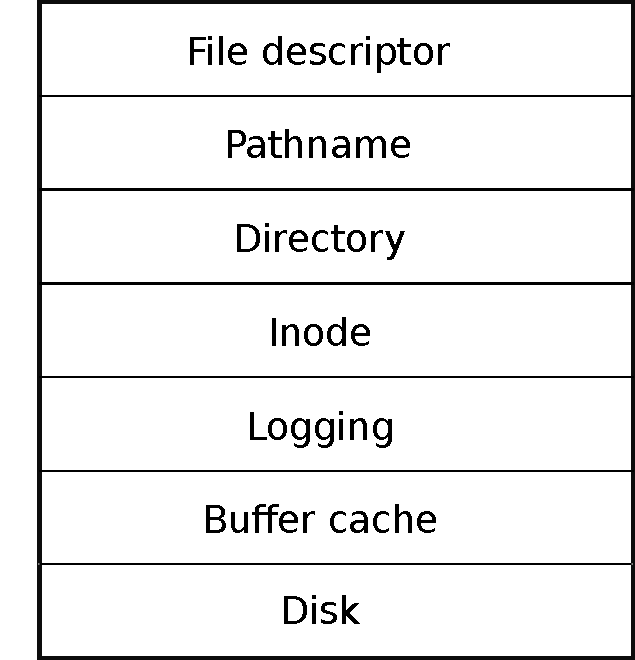
\includegraphics[scale=0.5]{fig/fslayer.pdf}
\caption{Layers of the xv6 file system.}
\label{fig:fslayer}
\end{figure}

The file system must have a plan for where it stores inodes and
content blocks on the disk.
To do so, xv6 divides the disk into several
sections, as shown in 
Figure~\ref{fig:fslayout}.
The file system does not use
block 0 (it holds the boot sector).  Block 1 is called the 
\indextext{superblock}; 
it contains metadata about the file system (the file system size in blocks, the
number of data blocks, the number of inodes, and the number of blocks in the
log).  Blocks starting at 2 hold the log.  After the log are the inodes, with multiple inodes per block.  After
those come bitmap blocks tracking which data blocks are in use.
The remaining blocks are data blocks; each is either marked
free in the bitmap block, or holds content for a file or directory.
The superblock is filled in by a separate program, called
\indexcode{mfks},
which builds an initial file system.

The rest of this chapter discusses each layer, starting with the
buffer cache.
Look out for situations where well-chosen abstractions at lower layers
ease the design of higher ones.
%% 
%%  -------------------------------------------
%% 
\section{Buffer cache layer}

The buffer cache has two jobs: (1) synchronize access to disk blocks to ensure
that only one copy of a block is in memory and that only one kernel thread at a time
uses that copy; (2) cache popular blocks so that they don't need to be re-read from
the slow disk. The code is in
\lstinline{bio.c}.

The main interface exported by the buffer cache consists of
\indexcode{bread}
and
\indexcode{bwrite};
the former obtains a
\indextext{buf}
containing a copy of a block which can be read or modified in memory, and the
latter writes a modified buffer to the appropriate block on the disk.
A kernel thread must release a buffer by calling
\indexcode{brelse}
when it is done with it.
The buffer cache uses a per-buffer sleep-lock to ensure
that only one thread at a time uses each buffer
(and thus each disk block);
\lstinline{bread}
returns a locked buffer, and
\lstinline{brelse}
releases the lock.

Let's return to the buffer cache.
The buffer cache has a fixed number of buffers to hold disk blocks,
which means that if the file system asks for a block that is not
already in the cache, the buffer cache must recycle a buffer currently
holding some other block. The buffer cache recycles the
least recently used buffer for the new block. The assumption is that
the least recently used buffer is the one least likely to be used
again soon.

\begin{figure}[t]
\center
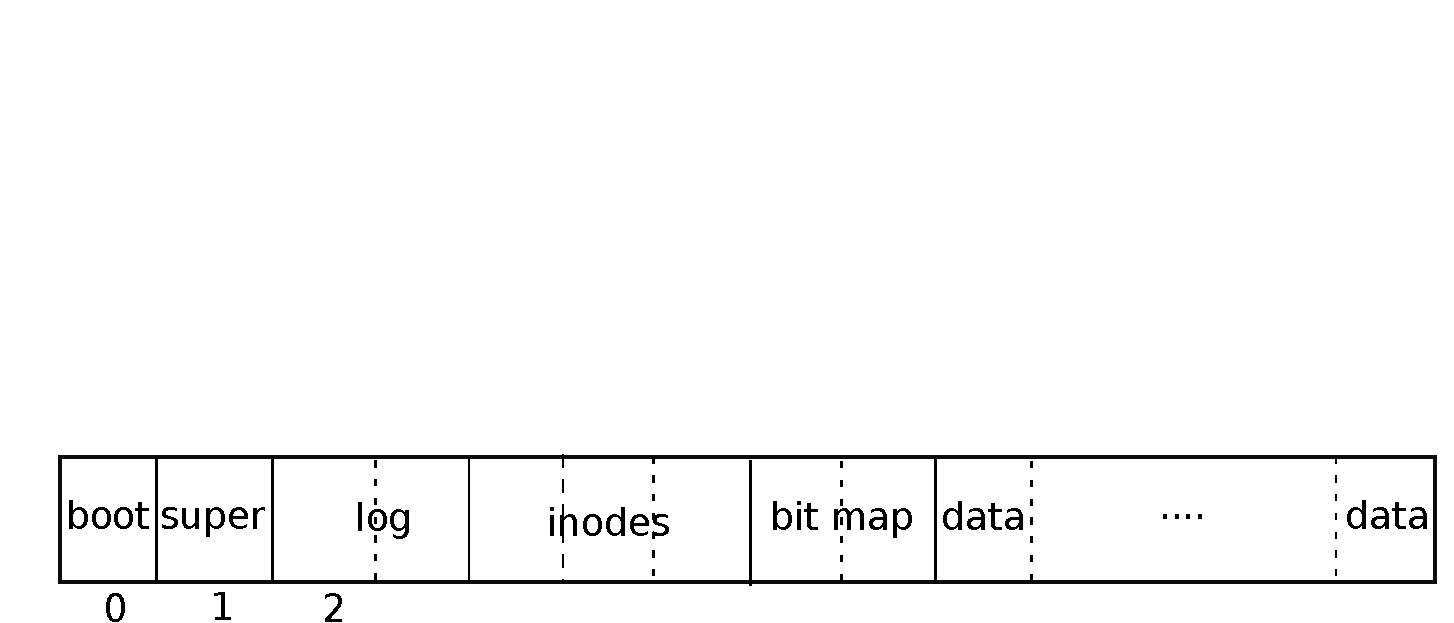
\includegraphics[scale=0.5]{fig/fslayout.pdf}
\caption{Structure of the xv6 file system. }
\label{fig:fslayout}
\end{figure}
%% 
%%  -------------------------------------------
%% 
\section{Code: Buffer cache}

The buffer cache is a doubly-linked list of buffers.
The function
\indexcode{binit},
called by
\indexcode{main}
\lineref{kernel/main.c:/binit/},
initializes the list with the
\indexcode{NBUF}
buffers in the static array
\lstinline{buf}
\linerefs{kernel/bio.c:/Create.linked.list/,/^..}/}.
All other access to the buffer cache refer to the linked list via
\indexcode{bcache.head},
not the
\lstinline{buf}
array.

A buffer has two state fields associated with it.
The field
\indexcode{valid}
indicates that the buffer contains a copy of the block.
The field \indexcode{disk}
indicates that the buffer content has been handed to
the disk, which may change the buffer (e.g., write
data from the disk into \lstinline{data}. 

\lstinline{Bread}
\lineref{kernel/bio.c:/^bread/}
calls
\indexcode{bget}
to get a buffer for the given sector
\lineref{kernel/bio.c:/b.=.bget/}.
If the buffer needs to be read from disk,
\lstinline{bread}
calls
\indexcode{virtio_disk_rw}
to do that before returning the buffer.

\lstinline{Bget}
\lineref{kernel/bio.c:/^bget/}
scans the buffer list for a buffer with the given device and sector numbers
\linerefs{kernel/bio.c:/Is.the.block.already/,/^..}/}.
If there is such a buffer,
\indexcode{bget}
acquires the sleep-lock for the buffer.
\lstinline{bget}
then returns the locked buffer.

If there is no cached buffer for the given sector,
\indexcode{bget}
must make one, possibly reusing a buffer that held
a different sector.
It scans the buffer list a second time, looking for a buffer
that is not in use (\lstinline{b->refcnt = 0}):
any such buffer can be used.
\lstinline{Bget}
edits the buffer metadata to record the new device and sector number
and acquires its sleep-lock.
Note that the assignment to
\lstinline{b->valid = 0}
ensures that
\lstinline{bread}
will read the block data from disk
rather than incorrectly using the buffer's previous contents.

It is important that there is at most one cached buffer per
disk sector, to ensure that readers see writes, and because the
file system uses locks on buffers for synchronization.
\lstinline{bget}
ensures this invariant by holding the
\lstinline{bache.lock}
continuously from the first loop's check of whether the
block is cached through the second loop's declaration that
the block is now cached (by setting
\lstinline{dev},
\lstinline{blockno},
and
\lstinline{refcnt}).
This causes the check for a block's presence and (if not
present) the designation of a buffer to hold the block to
be atomic.

It is safe for
\lstinline{bget}
to acquire the buffer's sleep-lock outside of the 
\lstinline{bcache.lock}
critical section,
since the non-zero
\lstinline{b->refcnt}
prevents the buffer from being re-used for a different disk block.
The sleep-lock protects reads
and writes of the block's buffered content, while the
\lstinline{bcache.lock}
protects information about which blocks are cached.

If all the buffers are busy, then too many processes are
simultaneously executing file system calls;
\lstinline{bget}
panics.
A more graceful response might be to sleep until a buffer became free,
though there would then be a possibility of deadlock.

Once
\indexcode{bread}
has read the disk (if needed) and returned the
buffer to its caller, the caller has
exclusive use of the buffer and can read or write the data bytes.
If the caller does modify the buffer, it must call
\indexcode{bwrite}
to write the changed data to disk before releasing the buffer.
\lstinline{Bwrite}
\lineref{kernel/bio.c:/^bwrite/}
calls
\indexcode{virtio_disk_rw}
to talk to the disk hardware.

When the caller is done with a buffer,
it must call
\indexcode{brelse}
to release it. 
(The name
\lstinline{brelse},
a shortening of
b-release,
is cryptic but worth learning:
it originated in Unix and is used in BSD, Linux, and Solaris too.)
\lstinline{Brelse}
\lineref{kernel/bio.c:/^brelse/}
releases the sleep-lock and
moves the buffer
to the front of the linked list
\linerefs{kernel/bio.c:/b->next->prev.=.b->prev/,/bcache.head.next.=.b/}.
Moving the buffer causes the
list to be ordered by how recently the buffers were used (meaning released):
the first buffer in the list is the most recently used,
and the last is the least recently used.
The two loops in
\lstinline{bget}
take advantage of this:
the scan for an existing buffer must process the entire list
in the worst case, but checking the most recently used buffers
first (starting at
\lstinline{bcache.head}
and following
\lstinline{next}
pointers) will reduce scan time when there is good locality of reference.
The scan to pick a buffer to reuse picks the least recently used
buffer by scanning backward
(following 
\lstinline{prev}
pointers).
%% 
%%  -------------------------------------------
%% 
\section{Logging layer}

One of the most interesting problems in file system design is crash
recovery. The problem arises because many file system operations
involve multiple writes to the disk, and a crash after a subset of the
writes may leave the on-disk file system in an inconsistent state. For
example, suppose a crash occurs during file truncation (setting
the length of a file to zero and freeing its content blocks).
Depending on the order of the disk writes, the crash 
may either leave an inode with a reference
to a content block that is marked free,
or it may leave an allocated but unreferenced content block.

The latter is relatively benign, but an inode that refers to a freed
block is likely to cause serious problems after a reboot.  After reboot, the
kernel might allocate that block to another file, and now we have two different
files pointing unintentionally to the same block.  If xv6 supported
multiple users, this situation could be a security problem, since the
old file's owner would be able to read and write blocks in the
new file, owned by a different user.

Xv6 solves the problem of crashes during file system operations with a
simple form of logging. An xv6 system call does not directly write
the on-disk file system data structures. Instead, it places a
description of all the disk writes it wishes to make in a 
\indextext{log} 
on the disk. Once the system call has logged all of its writes, it writes a
special 
\indextext{commit}
record to the disk indicating that the log contains
a complete operation. At that point the system call copies the writes
to the on-disk file system data structures. After those writes have
completed, the system call erases the log on disk.

If the system should crash and reboot, the file system code recovers
from the crash as follows, before running any processes. If the log is
marked as containing a complete operation, then the recovery code
copies the writes to where they belong in the on-disk file system. If
the log is not marked as containing a complete operation, the recovery
code ignores the log.  The recovery code finishes by erasing
the log.

Why does xv6's log solve the problem of crashes during file system
operations? If the crash occurs before the operation commits, then the
log on disk will not be marked as complete, the recovery code will
ignore it, and the state of the disk will be as if the operation had
not even started. If the crash occurs after the operation commits,
then recovery will replay all of the operation's writes, perhaps
repeating them if the operation had started to write them to the
on-disk data structure. In either case, the log makes operations
atomic with respect to crashes: after recovery, either all of the
operation's writes appear on the disk, or none of them appear.
%% 
%% 
%% 
\section{Log design}

The log resides at a known fixed location, specified in the superblock.
It consists of a header block followed by a sequence
of updated block copies (``logged blocks'').
The header block contains an array of sector
numbers, one for each of the logged blocks, and 
the count of log blocks.
The count in the header block on disk is either
zero, indicating that there is no transaction in the log,
or non-zero, indicating that the log contains a complete committed
transaction with the indicated number of logged blocks.
Xv6 writes the header
block when a transaction commits, but not before, and sets the
count to zero after copying the logged blocks to the file system.
Thus a crash midway through a transaction will result in a
count of zero in the log's header block; a crash after a commit
will result in a non-zero count.

Each system call's code indicates the start and end of the sequence of
writes that must be atomic with respect to crashes.
To allow concurrent execution of file system operations
by different processes,
the logging system can accumulate the writes
of multiple system calls into one transaction.
Thus a single commit may involve the writes of multiple
complete system calls.
To avoid splitting a system call across transactions, the logging system
only commits when no file system system calls are underway.

The idea of committing several transactions together is known as 
\indextext{group commit}.
Group commit reduces the number of disk operations
because it amortizes the fixed cost of a commit over multiple
operations.
Group commit also hands the disk system more concurrent writes
at the same time, perhaps allowing the disk to write
them all during a single disk rotation.
Xv6's virtio driver doesn't support this kind of
\indextext{batching},
but xv6's file system design allows for it.

Xv6 dedicates a fixed amount of space on the disk to hold the log.
The total number of blocks written by the system calls in a
transaction must fit in that space.
This has two consequences.
No single system call
can be allowed to write more distinct blocks than there is space
in the log. This is not a problem for most system calls, but two
of them can potentially write many blocks: 
\indexcode{write}
and
\indexcode{unlink}.
A large file write may write many data blocks and many bitmap blocks
as well as an inode block; unlinking a large file might write many
bitmap blocks and an inode.
Xv6's write system call breaks up large writes into multiple smaller
writes that fit in the log,
and 
\lstinline{unlink}
doesn't cause problems because in practice the xv6 file system uses
only one bitmap block.
The other consequence of limited log space
is that the logging system cannot allow a system call to start
unless it is certain that the system call's writes will
fit in the space remaining in the log.
%% 
%% 
%% 
\section{Code: logging}

A typical use of the log in a system call looks like this:
\begin{lstlisting}[]
  begin_op();
  ...
  bp = bread(...);
  bp->data[...] = ...;
  log_write(bp);
  ...
  end_op();
\end{lstlisting}

\indexcode{begin_op}
\lineref{kernel/log.c:/^begin.op/}
waits until
the logging system is not currently committing, and until
there is enough unreserved log space to hold
the writes from this call.
\lstinline{log.outstanding}
counts the number of system calls that have reserved log
space; the total reserved space is 
\lstinline{log.outstanding}
times
\lstinline{MAXOPBLOCKS}.
Incrementing
\lstinline{log.outstanding}
both reserves space and prevents a commit
from occuring during this system call.
The code conservatively assumes that each system call might write up to
\lstinline{MAXOPBLOCKS}
distinct blocks.

\indexcode{log_write}
\lineref{kernel/log.c:/^log.write/}
acts as a proxy for 
\indexcode{bwrite}.
It records the block's sector number in memory,
reserving it a slot in the log on disk,
and pins the buffer in the block cache
to prevent the block cache from evicting it.
The block must stay in the cache until committed:
until then, the cached copy is the only record
of the modification; it cannot be written to
its place on disk until after commit;
and other reads in the same transaction must
see the modifications.
\lstinline{log_write}
notices when a block is written multiple times during a single
transaction, and allocates that block the same slot in the log.
This optimization is often called
\indextext{absorption}.
It is common that, for example, the disk block containing inodes
of several files is written several times within a transaction.  By absorbing
several disk writes into one, the file system can save log space and
can achieve better performance because only one copy of the disk block must be
written to disk.

\indexcode{end_op}
\lineref{kernel/log.c:/^end.op/}
first decrements the count of outstanding system calls.
If the count is now zero, it commits the current
transaction by calling
\lstinline{commit().}
There are four stages in this process.
\lstinline{write_log()}
\lineref{kernel/log.c:/^write.log/}
copies each block modified in the transaction from the buffer
cache to its slot in the log on disk.
\lstinline{write_head()}
\lineref{kernel/log.c:/^write.head/}
writes the header block to disk: this is the
commit point, and a crash after the write will
result in recovery replaying the transaction's writes from the log.
\indexcode{install_trans}
\lineref{kernel/log.c:/^install_trans/}
reads each block from the log and writes it to the proper
place in the file system.
Finally
\lstinline{end_op}
writes the log header with a count of zero;
this has to happen before the next transaction starts writing
logged blocks, so that a crash doesn't result in recovery
using one transaction's header with the subsequent transaction's
logged blocks.

\indexcode{recover_from_log}
\lineref{kernel/log.c:/^recover_from_log/}
is called from 
\indexcode{initlog}
\lineref{kernel/log.c:/^initlog/},
which is called during boot before the first user process runs.
\lineref{kernel/proc.c:/initlog/}
It reads the log header, and mimics the actions of
\lstinline{end_op}
if the header indicates that the log contains a committed transaction.

An example use of the log occurs in 
\indexcode{filewrite}
\lineref{kernel/file.c:/^filewrite/}.
The transaction looks like this:
\begin{lstlisting}[]
      begin_op();
      ilock(f->ip);
      r = writei(f->ip, ...);
      iunlock(f->ip);
      end_op();
\end{lstlisting}
This code is wrapped in a loop that breaks up large writes into individual
transactions of just a few sectors at a time, to avoid overflowing
the log.  The call to
\indexcode{writei}
writes many blocks as part of this
transaction: the file's inode, one or more bitmap blocks, and some data
blocks.
%% 
%% 
%% 
\section{Code: Block allocator}

File and directory content is stored in disk blocks,
which must be allocated from a free pool.
xv6's block allocator
maintains a free bitmap on disk, with one bit per block. 
A zero bit indicates that the corresponding block is free;
a one bit indicates that it is in use.
The program
\lstinline{mkfs}
sets the bits corresponding to the boot sector, superblock, log blocks, inode
blocks, and bitmap blocks.

The block allocator provides two functions:
\indexcode{balloc}
allocates a new disk block, and
\indexcode{bfree}
frees a block.
\lstinline{Balloc}
The loop in
\lstinline{balloc}
at
\lineref{kernel/fs.c:/^..for.b.=.0/}
considers every block, starting at block 0 up to 
\lstinline{sb.size},
the number of blocks in the file system.
It looks for a block whose bitmap bit is zero,
indicating that it is free.
If
\lstinline{balloc}
finds such a block, it updates the bitmap 
and returns the block.
For efficiency, the loop is split into two 
pieces.
The outer loop reads each block of bitmap bits.
The inner loop checks all 
\lstinline{BPB}
bits in a single bitmap block.
The race that might occur if two processes try to allocate
a block at the same time is prevented by the fact that
the buffer cache only lets one process use any one bitmap block at a time.

\lstinline{Bfree}
\lineref{kernel/fs.c:/^bfree/}
finds the right bitmap block and clears the right bit.
Again the exclusive use implied by
\lstinline{bread}
and
\lstinline{brelse}
avoids the need for explicit locking.

As with much of the code described in the remainder of this chapter, 
\lstinline{balloc}
and
\lstinline{bfree}
must be called inside a transaction.
%% 
%%  -------------------------------------------
%% 
\section{Inode layer}

The term 
\indextext{inode} 
can have one of two related meanings.
It might refer to the on-disk data structure containing
a file's size and list of data block numbers.
Or ``inode'' might refer to an in-memory inode, which contains
a copy of the on-disk inode as well as extra information needed
within the kernel.

The on-disk inodes
are packed into a contiguous area
of disk called the inode blocks.
Every inode is the same size, so it is easy, given a
number n, to find the nth inode on the disk.
In fact, this number n, called the inode number or i-number,
is how inodes are identified in the implementation.

The on-disk inode is defined by a
\indexcode{struct dinode}
\lineref{kernel/fs.h:/^struct.dinode/}.
The 
\lstinline{type}
field distinguishes between files, directories, and special
files (devices).
A type of zero indicates that an on-disk inode is free.
The
\lstinline{nlink}
field counts the number of directory entries that
refer to this inode, in order to recognize when the
on-disk inode and its data blocks should be freed.
The
\lstinline{size}
field records the number of bytes of content in the file.
The
\lstinline{addrs}
array records the block numbers of the disk blocks holding
the file's content.

The kernel keeps the set of active inodes in memory;
\indexcode{struct inode}
\lineref{kernel/file.h:/^struct.inode/}
is the in-memory copy of a 
\lstinline{struct}
\lstinline{dinode}
on disk.
The kernel stores an inode in memory only if there are
C pointers referring to that inode. The
\lstinline{ref}
field counts the number of C pointers referring to the
in-memory inode, and the kernel discards the inode from
memory if the reference count drops to zero.
The
\indexcode{iget}
and
\indexcode{iput}
functions acquire and release pointers to an inode,
modifying the reference count.
Pointers to an inode can come from file descriptors,
current working directories, and transient kernel code
such as
\lstinline{exec}.

There are four lock or lock-like mechanisms in xv6's
inode code.
\lstinline{icache.lock}
protects the invariant that an inode is present in the cache
at most once, and the invariant that a cached inode's
\lstinline{ref}
field counts the number of in-memory pointers to the cached inode.
Each in-memory inode has a
\lstinline{lock}
field containing a
sleep-lock, which ensures exclusive access to the
inode's fields (such as file length) as well as to the
inode's file or directory content blocks.
An inode's
\lstinline{ref},
if it is greater than zero, causes the system to maintain
the inode in the cache, and not re-use the cache entry for
a different inode.
Finally, each inode contains a
\lstinline{nlink}
field (on disk and copied in memory if it is cached) that
counts the number of directory entries that refer to a file;
xv6 won't free an inode if its link count is greater than zero.

A
\lstinline{struct}
\lstinline{inode}
pointer returned by
\lstinline{iget()}
is guaranteed to be valid until the corresponding call to
\lstinline{iput()};
the inode won't be deleted, and the memory referred to
by the pointer won't be re-used for a different inode.
\lstinline{iget()}
provides non-exclusive access to an inode, so that
there can be many pointers to the same inode.
Many parts of the file system code depend on this behavior of
\lstinline{iget()},
both to hold long-term references to inodes (as open files
and current directories) and to prevent races while avoiding
deadlock in code that manipulates multiple inodes (such as
pathname lookup).

The
\lstinline{struct}
\lstinline{inode}
that 
\lstinline{iget}
returns may not have any useful content.
In order to ensure it holds a copy of the on-disk
inode, code must call
\indexcode{ilock}.
This locks the inode (so that no other process can
\lstinline{ilock}
it) and reads the inode from the disk,
if it has not already been read.
\lstinline{iunlock}
releases the lock on the inode.
Separating acquisition of inode pointers from locking
helps avoid deadlock in some situations, for example during
directory lookup.
Multiple processes can hold a C pointer to an inode
returned by 
\lstinline{iget},
but only one process can lock the inode at a time.

The inode cache only caches inodes to which kernel code
or data structures hold C pointers.
Its main job is really synchronizing access by multiple processes;
caching is secondary.
If an inode is used frequently, the buffer cache will probably
keep it in memory if it isn't kept by the inode cache.
The inode cache is \indextext{write-through}, which means that code that
modifies a cached inode must immediately write it to disk with
\lstinline{iupdate}.
%% 
%%  -------------------------------------------
%% 
\section{Code: Inodes}

To allocate a new inode (for example, when creating a file),
xv6 calls
\indexcode{ialloc}
\lineref{kernel/fs.c:/^ialloc/}.
\lstinline{Ialloc}
is similar to
\indexcode{balloc}:
it loops over the inode structures on the disk, one block at a time,
looking for one that is marked free.
When it finds one, it claims it by writing the new 
\lstinline{type}
to the disk and then returns an entry from the inode cache
with the tail call to 
\indexcode{iget}
\lineref{kernel/fs.c:/return.iget\(dev..inum\)/}.
The correct operation of
\lstinline{ialloc}
depends on the fact that only one process at a time
can be holding a reference to 
\lstinline{bp}:
\lstinline{ialloc}
can be sure that some other process does not
simultaneously see that the inode is available
and try to claim it.

\lstinline{Iget}
\lineref{kernel/fs.c:/^iget/}
looks through the inode cache for an active entry (\lstinline{ip->ref}
\lstinline{>}
\lstinline{0})
with the desired device and inode number.
If it finds one, it returns a new reference to that inode
\linerefs{kernel/fs.c:/^....if.ip->ref.>.0/,/^....}/}.
As
\indexcode{iget}
scans, it records the position of the first empty slot
\linerefs{kernel/fs.c:/^....if.empty.==.0/,/empty.=.ip/},
which it uses if it needs to allocate a cache entry.

Code must lock the inode using
\indexcode{ilock}
before reading or writing its metadata or content.
\lstinline{Ilock}
\lineref{kernel/fs.c:/^ilock/}
uses a sleep-lock for this purpose.
Once
\indexcode{ilock}
has exclusive access to the inode, it reads the inode
from disk (more likely, the buffer cache) if needed.
The function
\indexcode{iunlock}
\lineref{kernel/fs.c:/^iunlock/}
releases the sleep-lock,
which may cause any processes sleeping
to be woken up.

\lstinline{Iput}
\lineref{kernel/fs.c:/^iput/}
releases a C pointer to an inode
by decrementing the reference count
\lineref{kernel/fs.c:/^..ip->ref--/}.
If this is the last reference, the inode's
slot in the inode cache is now free and can be re-used
for a different inode.

If 
\indexcode{iput}
sees that there are no C pointer references to an inode
and that the inode has no links to it (occurs in no
directory), then the inode and its data blocks must
be freed.
\lstinline{Iput}
calls
\indexcode{itrunc}
to truncate the file to zero bytes, freeing the data blocks;
sets the inode type to 0 (unallocated);
and writes the inode to disk
\lineref{kernel/fs.c:/inode.has.no.links.and/}.

The locking protocol in 
\indexcode{iput}
in the case in which it frees the inode deserves a closer look.
One danger is that a concurrent thread might be waiting in
\lstinline{ilock}
to use this inode (e.g. to read a file or list a directory),
and won't be prepared to find the inode is not longer
allocated. This can't happen because there is no way for
a system call to get a pointer to a cached inode if it has
no links to it and 
\lstinline{ip->ref}
is one. That one reference is the reference owned by the
thread calling
\lstinline{iput}.
It's true that 
\lstinline{iput}
checks that the reference count is one outside of its
\lstinline{icache.lock}
critical section, but at that point the link
count is known to be zero, so no thread will try
to acquire a new reference.
The other main danger is that a concurrent call to
\lstinline{ialloc}
might choose the same inode that
\lstinline{iput}
is freeing.
This can only happen after the
\lstinline{iupdate}
writes the disk so that the inode has type zero.
This race is benign; the allocating thread will politely wait
to acquire the inode's sleep-lock before reading or writing
the inode, at which point
\lstinline{iput}
is done with it.

\lstinline{iput()}
can write to the disk.  This means that any system call that uses the file
system may write the disk, because the system call may be the last one having a
reference to the file. Even calls like
\lstinline{read()}
that appear to be read-only, may end up calling
\lstinline{iput().}
This, in turn, means that even read-only system calls
must be wrapped in transactions if they use the file system.

There is a challenging interaction between
\lstinline{iput()}
and crashes.
\lstinline{iput()}
doesn't truncate a file immediately when the link count for the file
drops to zero, because some process might still hold a reference to the inode in
memory: a process might still be reading and writing to the file, because it
successfully opened it. But, if a crash happens before the last process closes
the file descriptor for the file, then the file will be marked allocated on disk
but no directory entry points to it.

File systems handle this case in one of two ways. The simple solution is that on
recovery, after reboot, the file system scans the whole file system for files
that are marked allocated, but have no directory entry pointing to them.  If any
such file exists, then it can free those files.

The second solution doesn't require scanning the file system.  In this solution,
the file system records on disk (e.g., in the super block) the inode inumber of
a file whose link count drops to zero but whose reference count isn't zero.  If
the file system removes the file when its reference counts reaches 0, then it
updates the on-disk list by removing that inode from the list. On recovery, the
file system frees any file in the list.

Xv6 implements neither solution, which means that inodes may be marked allocated
on disk, even though they are not in use anymore.  This means that over time xv6
runs the risk that it may run out of disk space.
%% 
%% 
%% 
\section{Code: Inode content}

\begin{figure}[t]
\center
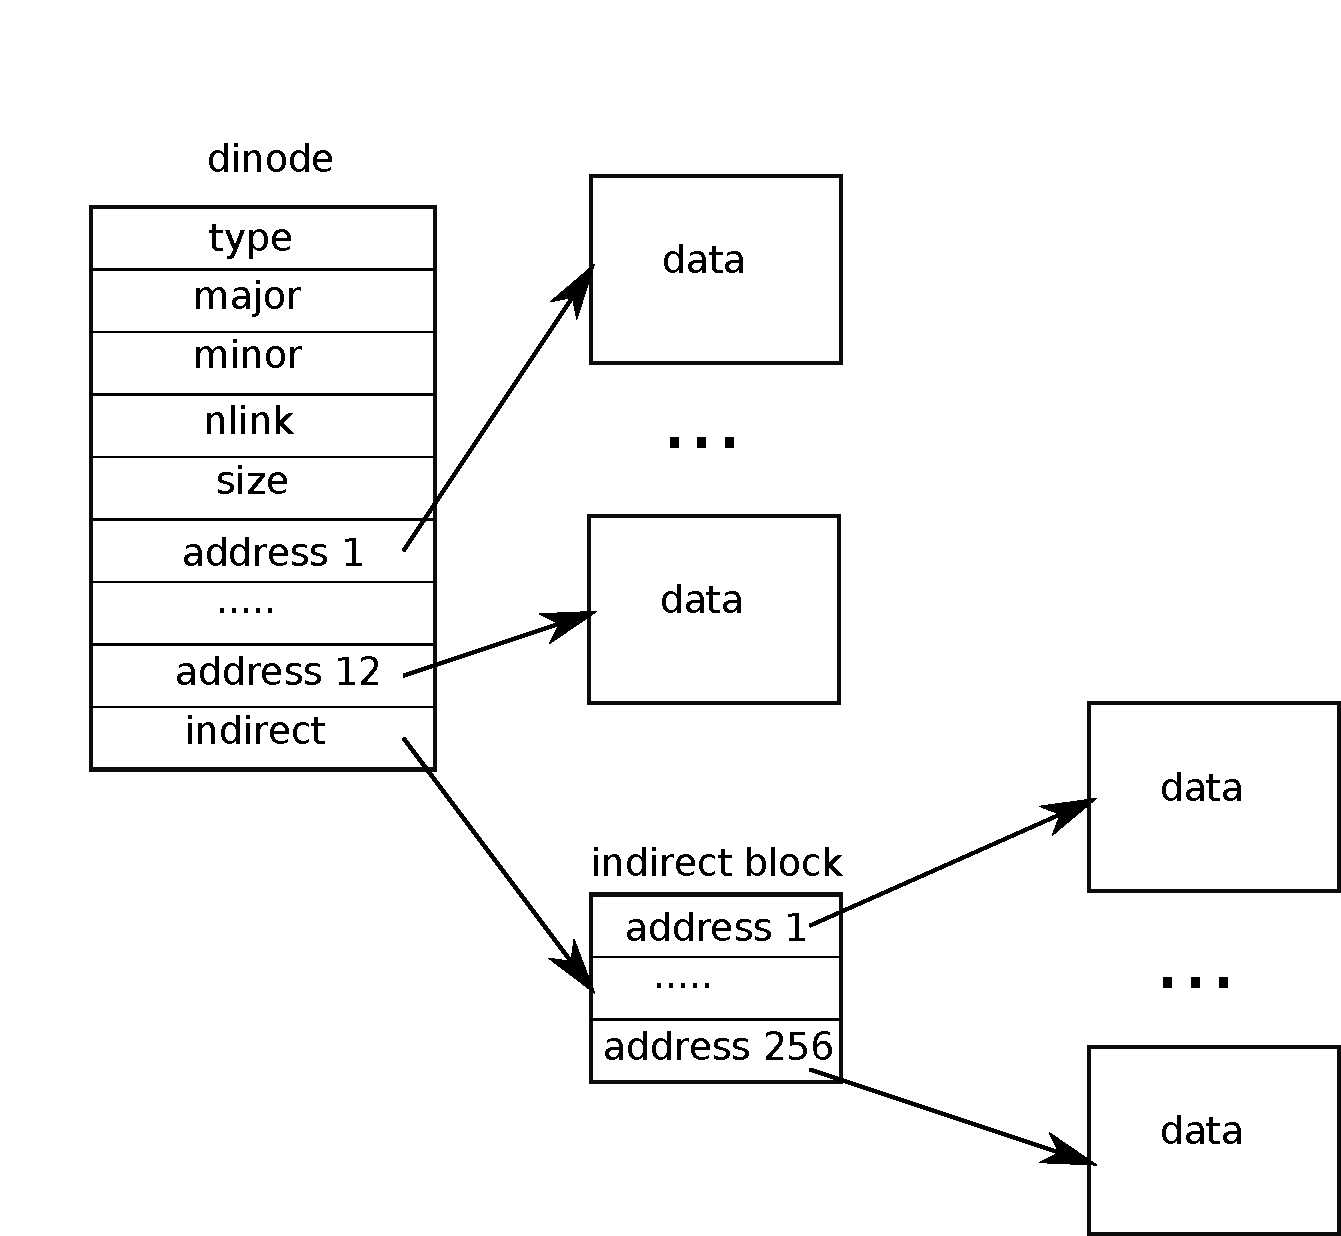
\includegraphics[scale=0.5]{fig/inode.pdf}
\caption{The representation of a file on disk.}
\label{fig:inode}
\end{figure}

The on-disk inode structure,
\indexcode{struct dinode},
contains a size and an array of block numbers (see 
Figure~\ref{fig:inode}).
The inode data is found in the blocks listed
in the
\lstinline{dinode} 's
\lstinline{addrs}
array.
The first
\indexcode{NDIRECT}
blocks of data are listed in the first
\lstinline{NDIRECT}
entries in the array; these blocks are called 
\indextext{direct blocks}.
The next 
\indexcode{NINDIRECT}
blocks of data are listed not in the inode
but in a data block called the
\indextext{indirect block}.
The last entry in the
\lstinline{addrs}
array gives the address of the indirect block.
Thus the first 12 kB (
\lstinline{NDIRECT} 
\lstinline{x}
\indexcode{BSIZE})
bytes of a file can be loaded from blocks listed in the inode,
while the next
\lstinline{256} kB (
\lstinline{NINDIRECT}
\lstinline{x}
\lstinline{BSIZE})
bytes can only be loaded after consulting the indirect block.
This is a good on-disk representation but a 
complex one for clients.
The function
\indexcode{bmap}
manages the representation so that higher-level routines such as
\indexcode{readi}
and
\indexcode{writei},
which we will see shortly.
\lstinline{Bmap}
returns the disk block number of the
\lstinline{bn} 'th
data block for the inode
\lstinline{ip}.
If
\lstinline{ip}
does not have such a block yet,
\lstinline{bmap}
allocates one.

The function
\indexcode{bmap}
\lineref{kernel/fs.c:/^bmap/}
begins by picking off the easy case: the first 
\indexcode{NDIRECT}
blocks are listed in the inode itself
\linerefs{kernel/fs.c:/^..if.bn.<.NDIRECT/,/^..}/}.
The next 
\indexcode{NINDIRECT}
blocks are listed in the indirect block at
\lstinline{ip->addrs[NDIRECT]}.
\lstinline{Bmap}
reads the indirect block
\lineref{kernel/fs.c:/bp.=.bread.ip->dev..addr/}
and then reads a block number from the right 
position within the block
\lineref{kernel/fs.c:/a.=..uint\*.bp->data/}.
If the block number exceeds
\lstinline{NDIRECT}+NINDIRECT,
\lstinline{bmap} 
panics; 
\lstinline{writei}
contains the check that prevents this from happening
\lineref{kernel/fs.c:/off...n...MAXFILE.BSIZE/}.

\lstinline{Bmap}
allocates blocks as needed.
An
\lstinline{ip->addrs[]}
or indirect
entry of zero indicates that no block is allocated.
As
\lstinline{bmap}
encounters zeros, it replaces them with the numbers of fresh blocks,
allocated on demand
\linerefs{kernel/fs.c:/^....if..addr.=.*==.0/,/./}
\linerefs{kernel/fs.c:/^....if..addr.*NDIRECT.*==.0/,/./}.

\indexcode{itrunc}
frees a file's blocks, resetting the inode's size to zero.
\lstinline{Itrunc}
\lineref{kernel/fs.c:/^itrunc/}
starts by freeing the direct blocks
\linerefs{kernel/fs.c:/^..for.i.=.0.*NDIRECT/,/^..}/},
then the ones listed in the indirect block
\linerefs{kernel/fs.c:/^....for.j.=.0.*NINDIRECT/,/^....}/},
and finally the indirect block itself
\linerefs{kernel/fs.c:/^....bfree.*NDIRECT/,/./}.

\lstinline{Bmap}
makes it easy for
\indexcode{readi}
and
\indexcode{writei} 
to get at an inode's data.
\lstinline{Readi}
\lineref{kernel/fs.c:/^readi/}
starts by
making sure that the offset and count are not 
beyond the end of the file.
Reads that start beyond the end of the file return an error
\linerefs{kernel/fs.c:/^..if.off.>.ip->size/,/./}
while reads that start at or cross the end of the file 
return fewer bytes than requested
\linerefs{kernel/fs.c:/^..if.off.\+.n.>.ip->size/,/./}.
The main loop processes each block of the file,
copying data from the buffer into 
\lstinline{dst}
\linerefs{kernel/fs.c:/^..for.tot=0/,/^..}/}.
%%  NOTE: It is very hard to write line references
%%  for writei because so many of the lines are identical
%%  to those in readi.  Luckily, identical lines probably
%%  don't need to be commented upon.
\indexcode{writei}
\lineref{kernel/fs.c:/^writei/}
is identical to
\indexcode{readi},
with three exceptions:
writes that start at or cross the end of the file
grow the file, up to the maximum file size
\linerefs{kernel/fs.c:/^..if.off.\+.n.>.MAXFILE/,/./};
the loop copies data into the buffers instead of out
\lineref{kernel/fs.c:/memmove.bp->data/};
and if the write has extended the file,
\indexcode{writei}
must update its size
\lineref{kernel/fs.c:/^..if.n.>.0.*off.>.ip->size/,/^..}/}.

Both
\indexcode{readi}
and
\indexcode{writei}
begin by checking for
\lstinline{ip->type}
\lstinline{==}
\indexcode{T_DEV}.
This case handles special devices whose data does not
live in the file system; we will return to this case in the file descriptor layer.

The function
\indexcode{stati}
\lineref{kernel/fs.c:/^stati\(/}
copies inode metadata into the 
\lstinline{stat}
structure, which is exposed to user programs
via the
\indexcode{stat}
system call.
%% 
%% 
%% 
\section{Code: directory layer}

A directory is implemented internally much like a file.
Its inode has type
\indexcode{T_DIR}
and its data is a sequence of directory entries.
Each entry is a
\indexcode{struct dirent}
\lineref{kernel/fs.h:/^struct.dirent/},
which contains a name and an inode number.
The name is at most
\indexcode{DIRSIZ}
(14) characters;
if shorter, it is terminated by a NUL (0) byte.
Directory entries with inode number zero are free.

The function
\indexcode{dirlookup}
\lineref{kernel/fs.c:/^dirlookup/}
searches a directory for an entry with the given name.
If it finds one, it returns a pointer to the corresponding inode, unlocked,
and sets 
\lstinline{*poff}
to the byte offset of the entry within the directory,
in case the caller wishes to edit it.
If
\lstinline{dirlookup}
finds an entry with the right name,
it updates
\lstinline{*poff}
and returns an unlocked inode
obtained via
\indexcode{iget}.
\lstinline{Dirlookup}
is the reason that 
\lstinline{iget}
returns unlocked inodes.
The caller has locked
\lstinline{dp},
so if the lookup was for
\indexcode{.},
an alias for the current directory,
attempting to lock the inode before
returning would try to re-lock
\lstinline{dp}
and deadlock.
(There are more complicated deadlock scenarios involving
multiple processes and
\indexcode{..},
an alias for the parent directory;
\lstinline{.}
is not the only problem.)
The caller can unlock
\lstinline{dp}
and then lock
\lstinline{ip},
ensuring that it only holds one lock at a time.

The function
\indexcode{dirlink}
\lineref{kernel/fs.c:/^dirlink/}
writes a new directory entry with the given name and inode number into the
directory
\lstinline{dp}.
If the name already exists,
\lstinline{dirlink}
returns an error
\linerefs{kernel/fs.c:/Check.that.name.is.not.present/,/^..}/}.
The main loop reads directory entries looking for an unallocated entry.
When it finds one, it stops the loop early
\linerefs{kernel/fs.c:/^....if.de.inum.==.0/,/./},
with 
\lstinline{off}
set to the offset of the available entry.
Otherwise, the loop ends with
\lstinline{off}
set to
\lstinline{dp->size}.
Either way, 
\lstinline{dirlink}
then adds a new entry to the directory
by writing at offset
\lstinline{off}
\linerefs{kernel/fs.c:/^..strncpy/,/panic/}.
%% 
%% 
%% 
\section{Code: Path names}

Path name lookup involves a succession of calls to
\indexcode{dirlookup},
one for each path component.
\lstinline{Namei}
\lineref{kernel/fs.c:/^namei/}
evaluates 
\lstinline{path}
and returns the corresponding 
\lstinline{inode}.
The function
\indexcode{nameiparent}
is a variant: it stops before the last element, returning the 
inode of the parent directory and copying the final element into
\lstinline{name}.
Both call the generalized function
\indexcode{namex}
to do the real work.

\lstinline{Namex}
\lineref{kernel/fs.c:/^namex/}
starts by deciding where the path evaluation begins.
If the path begins with a slash, evaluation begins at the root;
otherwise, the current directory
\linerefs{kernel/fs.c:/..if.\*path.==....\)/,/idup/}.
Then it uses
\indexcode{skipelem}
to consider each element of the path in turn
\lineref{kernel/fs.c:/while.*skipelem/}.
Each iteration of the loop must look up 
\lstinline{name}
in the current inode
\lstinline{ip}.
The iteration begins by locking
\lstinline{ip}
and checking that it is a directory.
If not, the lookup fails
\linerefs{kernel/fs.c:/^....ilock.ip/,/^....}/}.
(Locking
\lstinline{ip}
is necessary not because 
\lstinline{ip->type}
can change underfoot—it can't—but because
until 
\indexcode{ilock}
runs,
\lstinline{ip->type}
is not guaranteed to have been loaded from disk.)
If the call is 
\indexcode{nameiparent}
and this is the last path element, the loop stops early,
as per the definition of
\lstinline{nameiparent};
the final path element has already been copied
into
\lstinline{name},
so
\indexcode{namex}
need only
return the unlocked
\lstinline{ip}
\linerefs{kernel/fs.c:/^....if.nameiparent/,/^....}/}.
Finally, the loop looks for the path element using
\indexcode{dirlookup}
and prepares for the next iteration by setting
\lstinline{ip = next}
\linerefs{kernel/fs.c:/^....if..next.*dirlookup/,/^....ip.=.next/}.
When the loop runs out of path elements, it returns
\lstinline{ip}.

The procedure
\lstinline{namex}
may take a long time to complete: it could involve several disk operations to
read inodes and directory blocks for the directories traversed in the pathname
(if they are not in the buffer cache).  Xv6 is carefully designed so that if an
invocation of
\lstinline{namex}
by one kernel thread is blocked on a disk I/O, another kernel thread looking up
a different pathname can proceed concurrently.
\lstinline{namex}
locks each directory in the path separately so that lookups in different
directories can proceed in parallel.

This concurrency introduces some challenges. For example, while one kernel
thread is looking up a pathname another kernel thread may be changing the
directory tree by unlinking a directory.  A potential risk is that a lookup
may be searching a directory that has been deleted by another kernel thread and
its blocks have been re-used for another directory or file.

Xv6 avoids such races.  For example, when executing
\lstinline{dirlookup}
in
\lstinline{namex},
the lookup thread holds the lock on the directory and
\lstinline{dirlookup}
returns an inode that was obtained using
\lstinline{iget}.
\lstinline{iget}
increases the reference count of the inode.  Only after receiving the
inode from
\lstinline{dirlookup}
does
\lstinline{namex}
release the lock on the directory.  Now another thread may unlink the inode from
the directory but xv6 will not delete the inode yet, because the reference count
of the inode is still larger than zero.

Another risk is deadlock.  For example,
\lstinline{next}
points to the same inode as
\lstinline{ip}
when looking up ".".
Locking
\lstinline{next}
before releasing the lock on
\lstinline{ip}
would result in a deadlock.
To avoid this deadlock,
\lstinline{namex}
unlocks the directory before obtaining a lock on
\lstinline{next}.
Here again we see why the separation between
\lstinline{iget}
and
\lstinline{ilock}
is important.
%% 
%% 
%% 
\section{File descriptor layer}

A cool aspect of the Unix interface is that most resources in Unix are
represented as files, including devices such as the console, pipes, and of
course, real files.  The file descriptor layer is the layer that achieves this
uniformity.

Xv6 gives each process its own table of open files, or
file descriptors, as we saw in
Chapter~\ref{CH:UNIX}.
Each open file is represented by a
\indexcode{struct file}
\lineref{kernel/file.h:/^struct.file/},
which is a wrapper around either an inode or a pipe,
plus an i/o offset.
Each call to 
\indexcode{open}
creates a new open file (a new
\lstinline{struct}
\lstinline{file}):
if multiple processes open the same file independently,
the different instances will have different i/o offsets.
On the other hand, a single open file
(the same
\lstinline{struct}
\lstinline{file})
can appear
multiple times in one process's file table
and also in the file tables of multiple processes.
This would happen if one process used
\lstinline{open}
to open the file and then created aliases using
\indexcode{dup}
or shared it with a child using
\indexcode{fork}.
A reference count tracks the number of references to
a particular open file.
A file can be open for reading or writing or both.
The
\lstinline{readable}
and
\lstinline{writable}
fields track this.

All the open files in the system are kept in a global file table,
the 
\indexcode{ftable}.
The file table
has a function to allocate a file
(\indexcode{filealloc}),
create a duplicate reference
(\indexcode{filedup}),
release a reference
(\indexcode{fileclose}),
and read and write data
\indexcode{fileread} "" (
and 
\indexcode{filewrite}).

The first three follow the now-familiar form.
\lstinline{Filealloc}
\lineref{kernel/file.c:/^filealloc/}
scans the file table for an unreferenced file
\lstinline{f->ref} "" (
\lstinline{==}
\lstinline{0})
and returns a new reference;
\indexcode{filedup}
\lineref{kernel/file.c:/^filedup/}
increments the reference count;
and
\indexcode{fileclose}
\lineref{kernel/file.c:/^fileclose/}
decrements it.
When a file's reference count reaches zero,
\lstinline{fileclose}
releases the underlying pipe or inode,
according to the type.

The functions
\indexcode{filestat},
\indexcode{fileread},
and
\indexcode{filewrite}
implement the 
\indexcode{stat},
\indexcode{read},
and
\indexcode{write}
operations on files.
\lstinline{Filestat}
\lineref{kernel/file.c:/^filestat/}
is only allowed on inodes and calls
\indexcode{stati}.
\lstinline{Fileread}
and
\lstinline{filewrite}
check that the operation is allowed by
the open mode and then
pass the call through to either
the pipe or inode implementation.
If the file represents an inode,
\lstinline{fileread}
and
\lstinline{filewrite}
use the i/o offset as the offset for the operation
and then advance it
\linerefs{kernel/file.c:/readi/,/./}
\linerefs{kernel/file.c:/writei/,/./}.
Pipes have no concept of offset.
Recall that the inode functions require the caller
to handle locking
\linerefs{kernel/file.c:/stati/-1,/iunlock/}
\linerefs{kernel/file.c:/readi/-1,/iunlock/}
\linerefs{kernel/file.c:/writei\(f/-1,/iunlock/}.
The inode locking has the convenient side effect that the
read and write offsets are updated atomically, so that
multiple writing to the same file simultaneously
cannot overwrite each other's data, though their writes may end up interlaced.
%% 
%% 
%% 
\section{Code: System calls}

With the functions that the lower layers provide the implementation of most
system calls is trivial
(see
\fileref{kernel/sysfile.c}).
There are a few calls that
deserve a closer look.

The functions
\indexcode{sys_link}
and
\indexcode{sys_unlink}
edit directories, creating or removing references to inodes.
They are another good example of the power of using 
transactions. 
\lstinline{Sys_link}
\lineref{kernel/sysfile.c:/^sys_link/}
begins by fetching its arguments, two strings
\lstinline{old}
and
\lstinline{new}
\lineref{kernel/sysfile.c:/argstr.*old.*new/}.
Assuming 
\lstinline{old}
exists and is not  a directory
\linerefs{kernel/sysfile.c:/namei.old/,/^..}/},
\lstinline{sys_link}
increments its 
\lstinline{ip->nlink}
count.
Then
\lstinline{sys_link}
calls
\indexcode{nameiparent}
to find the parent directory and final path element of
\lstinline{new} 
\lineref{kernel/sysfile.c:/nameiparent.new/}
and creates a new directory entry pointing at
\lstinline{old} 's
inode
\lineref{kernel/sysfile.c:/\|\| dirlink/}.
The new parent directory must exist and
be on the same device as the existing inode:
inode numbers only have a unique meaning on a single disk.
If an error like this occurs, 
\indexcode{sys_link}
must go back and decrement
\lstinline{ip->nlink}.

Transactions simplify the implementation because it requires updating multiple
disk blocks, but we don't have to worry about the order in which we do
them. They either will all succeed or none.
For example, without transactions, updating
\lstinline{ip->nlink}
before creating a link, would put the file system temporarily in an unsafe
state, and a crash in between could result in havoc.
With transactions we don't have to worry about this.

\lstinline{Sys_link}
creates a new name for an existing inode.
The function
\indexcode{create}
\lineref{kernel/sysfile.c:/^create/}
creates a new name for a new inode.
It is a generalization of the three file creation
system calls:
\indexcode{open}
with the
\indexcode{O_CREATE}
flag makes a new ordinary file,
\indexcode{mkdir}
makes a new directory,
and
\indexcode{mkdev}
makes a new device file.
Like
\indexcode{sys_link},
\indexcode{create}
starts by caling
\indexcode{nameiparent}
to get the inode of the parent directory.
It then calls
\indexcode{dirlookup}
to check whether the name already exists
\lineref{kernel/sysfile.c:/dirlookup.*[^=]=.0/}.
If the name does exist, 
\lstinline{create} 's
behavior depends on which system call it is being used for:
\lstinline{open}
has different semantics from 
\indexcode{mkdir}
and
\indexcode{mkdev}.
If
\lstinline{create}
is being used on behalf of
\lstinline{open}
\lstinline{type} "" (
\lstinline{==}
\indexcode{T_FILE})
and the name that exists is itself
a regular file,
then 
\lstinline{open}
treats that as a success,
so
\lstinline{create}
does too
\lineref{kernel/sysfile.c:/^......return.ip/}.
Otherwise, it is an error
\linerefs{kernel/sysfile.c:/^......return.ip/+1,/return.0/}.
If the name does not already exist,
\lstinline{create}
now allocates a new inode with
\indexcode{ialloc}
\lineref{kernel/sysfile.c:/ialloc/}.
If the new inode is a directory, 
\lstinline{create}
initializes it with
\indexcode{.}
and
\indexcode{..}
entries.
Finally, now that the data is initialized properly,
\indexcode{create}
can link it into the parent directory
\lineref{kernel/sysfile.c:/if.dirlink/}.
\lstinline{Create},
like
\indexcode{sys_link},
holds two inode locks simultaneously:
\lstinline{ip}
and
\lstinline{dp}.
There is no possibility of deadlock because
the inode
\lstinline{ip}
is freshly allocated: no other process in the system
will hold 
\lstinline{ip} 's
lock and then try to lock
\lstinline{dp}.

Using
\lstinline{create},
it is easy to implement
\indexcode{sys_open},
\indexcode{sys_mkdir},
and
\indexcode{sys_mknod}.
\lstinline{Sys_open}
\lineref{kernel/sysfile.c:/^sys_open/}
is the most complex, because creating a new file is only
a small part of what it can do.
If
\indexcode{open}
is passed the
\indexcode{O}\_CREATE
flag, it calls
\lstinline{create}
\lineref{kernel/sysfile.c:/create.*T_FILE/}.
Otherwise, it calls
\indexcode{namei}
\lineref{kernel/sysfile.c:/if..ip.=.namei.path/}.
\lstinline{Create}
returns a locked inode, but 
\lstinline{namei}
does not, so
\indexcode{sys_open}
must lock the inode itself.
This provides a convenient place to check that directories
are only opened for reading, not writing.
Assuming the inode was obtained one way or the other,
\lstinline{sys_open}
allocates a file and a file descriptor
\lineref{kernel/sysfile.c:/filealloc.*fdalloc/}
and then fills in the file
\linerefs{kernel/sysfile.c:/type.=.FD_INODE/,/writable/}.
Note that no other process can access the partially initialized file since it is only
in the current process's table.

Chapter~\ref{CH:SCHED} examined the implementation of pipes
before we even had a file system.
The function
\indexcode{sys_pipe}
connects that implementation to the file system
by providing a way to create a pipe pair.
Its argument is a pointer to space for two integers,
where it will record the two new file descriptors.
Then it allocates the pipe and installs the file descriptors.
%% 
%%  -------------------------------------------
%% 
\section{Real world}

The buffer cache in a real-world operating system is significantly
more complex than xv6's, but it serves the same two purposes:
caching and synchronizing access to the disk.
Xv6's buffer cache, like V6's, uses a simple least recently used (LRU)
eviction policy; there are many more complex
policies that can be implemented, each good for some
workloads and not as good for others.
A more efficient LRU cache would eliminate the linked list,
instead using a hash table for lookups and a heap for LRU evictions.
Modern buffer caches are typically integrated with the
virtual memory system to support memory-mapped files.

Xv6's logging system is inefficient.
A commit cannot occur concurrently with file system system calls.
The system logs entire blocks, even if
only a few bytes in a block are changed. It performs synchronous
log writes, a block at a time, each of which is likely to require an
entire disk rotation time. Real logging systems address all of these
problems.

Logging is not the only way to provide crash recovery. Early file systems
used a scavenger during reboot (for example, the UNIX
\indexcode{fsck}
program) to examine every file and directory and the block and inode
free lists, looking for and resolving inconsistencies. Scavenging can take
hours for large file systems, and there are situations where it is not
possible to resolve inconsistencies in a way that causes the original
system calls to be atomic. Recovery
from a log is much faster and causes system calls to be atomic
in the face of crashes.

Xv6 uses the same basic on-disk layout of inodes and directories
as early UNIX;
this scheme has been remarkably persistent over the years.
BSD's UFS/FFS and Linux's ext2/ext3 use essentially the same data structures.
The most inefficient part of the file system layout is the directory,
which requires a linear scan over all the disk blocks during each lookup.
This is reasonable when directories are only a few disk blocks,
but is expensive for directories holding many files.
Microsoft Windows's NTFS, Mac OS X's HFS, and Solaris's ZFS, just to name a few, implement
a directory as an on-disk balanced tree of blocks.
This is complicated but guarantees logarithmic-time directory lookups.

Xv6 is naive about disk failures: if a disk
operation fails, xv6 panics.
Whether this is reasonable depends on the hardware:
if an operating systems sits atop special hardware that uses
redundancy to mask disk failures, perhaps the operating system
sees failures so infrequently that panicking is okay.
On the other hand, operating systems using plain disks
should expect failures and handle them more gracefully,
so that the loss of a block in one file doesn't affect the
use of the rest of the file system.

Xv6 requires that the file system
fit on one disk device and not change in size.
As large databases and multimedia files drive storage
requirements ever higher, operating systems are developing ways
to eliminate the ``one disk per file system'' bottleneck.
The basic approach is to combine many disks into a single
logical disk.  Hardware solutions such as RAID are still the 
most popular, but the current trend is moving toward implementing
as much of this logic in software as possible.
These software implementations typically 
allow rich functionality like growing or shrinking the logical
device by adding or removing disks on the fly.
Of course, a storage layer that can grow or shrink on the fly
requires a file system that can do the same: the fixed-size array
of inode blocks used by xv6 would not work well
in such environments.
Separating disk management from the file system may be
the cleanest design, but the complex interface between the two
has led some systems, like Sun's ZFS, to combine them.

Xv6's file system lacks many other features of modern file systems; for example,
it lacks support for snapshots and incremental backup.

Modern Unix systems allow many kinds of resources to be
accessed with the same system calls as on-disk storage:
named pipes, network connections,
remotely-accessed network file systems, and monitoring and control
interfaces such as
\lstinline{/proc}.
Instead of xv6's
\lstinline{if}
statements in
\indexcode{fileread}
and
\indexcode{filewrite},
these systems typically give each open file a table of function pointers,
one per operation,
and call the function pointer to invoke that inode's
implementation of the call.
Network file systems and user-level file systems 
provide functions that turn those calls into network RPCs
and wait for the response before returning.
%% 
%%  -------------------------------------------
%% 
\section{Exercises}

\begin{enumerate}

\item Why panic in
\lstinline{balloc} ?
Can xv6 recover?

\item Why panic in
\lstinline{ialloc} ?
Can xv6 recover?

\item Why doesn't
\lstinline{filealloc}
panic when it runs out of files?
Why is this more common and therefore worth handling?

\item Suppose the file corresponding to 
\lstinline{ip}
gets unlinked by another process
between 
\lstinline{sys_link} 's
calls to 
\lstinline{iunlock(ip)}
and
\lstinline{dirlink}.
Will the link be created correctly?
Why or why not?

\item
\lstinline{create}
makes four function calls (one to
\lstinline{ialloc}
and three to
\lstinline{dirlink})
that it requires to succeed.
If any doesn't,
\lstinline{create}
calls
\lstinline{panic}.
Why is this acceptable?
Why can't any of those four calls fail?

\item
\lstinline{sys_chdir}
calls
\lstinline{iunlock(ip)}
before
\lstinline{iput(cp->cwd)},
which might try to lock
\lstinline{cp->cwd},
yet postponing
\lstinline{iunlock(ip)}
until after the
\lstinline{iput}
would not cause deadlocks.
Why not?

\item Implement the
\lstinline{lseek}
system call.  Supporting
\lstinline{lseek}
will also require that you modify
\lstinline{filewrite}
to fill holes in the file with zero if
\lstinline{lseek}
sets
\lstinline{off}
beyond
\lstinline{f->ip->size.}

\item Add
\lstinline{O_TRUNC}
and
\lstinline{O_APPEND}
to
\lstinline{open},
so that
\lstinline{>}
and
\lstinline{>>}
operators work in the shell.

\item Modify the file system to support symbolic links.

\item Modify the file system to support names pipes.

\item Modify the file and VM system to support mmap.

\end{enumerate}

\chapter{Summary}
\label{CH:SUM}

This text introduced the main ideas in operating systems by studying one
operating system, xv6, line by line.  Some code lines embody the essence of the
main ideas (e.g., context switching, user/kernel boundary, locks, etc.) and each
line is important; other code lines provide an illustration of how to implement
a particular operating system idea and could easily be done in different ways
(e.g., a better algorithm for scheduling, better on-disk data structures to
represent files, better logging to allow for concurrent transactions, etc.).
All the ideas were illustrated in the context of one particular, very successful
system call interface, the Unix interface, but those ideas carry over to the
design of other operating systems.



{
% The following prevents latex from splitting a bibliography entry with a page
% break
\interlinepenalty=10000
% Since we're using natbib in numbers mode, we don't need plainnat,
% which exists to feed authors and years back in to natbib.  As a
% result, it complains about entries without years, which we don't
% care about.
%\bibliographystyle{plainnat}
\bibliographystyle{plain}
\bibliography{book}
}

\printindex

\end{document}
